\documentclass[UTF8]{ctexart}
\usepackage{amsmath}
\usepackage{diagbox}
\usepackage{textcomp}
\usepackage{graphicx}
\usepackage{float}
\usepackage{caption}
\usepackage{adjustbox}
\usepackage{subfigure}
\usepackage{geometry}
\usepackage{pifont}
\usepackage{chngpage}
\usepackage{bm}
\begin{document}
\renewcommand{\thefootnote}{\fnsymbol{footnote}}
\newgeometry{left=2.5cm,bottom=4cm,right=2.5cm}
%\pagestyle{plain}
\linespread{1.4}
\title{\vspace{-5em}\heiti两位二进制数运算电路实验报告\vspace{-2.5em}}
\date{}
\maketitle
\begin{center}
{\fangsong 徐浩博\quad 软件02\quad2020010108}
\end{center}

\subsubsection*{摘要}
{\kaishu\normalsize  本实验旨在通过在实验板上实现加法器和减法器,使我们更加深入理解组合逻辑电路的设计、实现、故障排查等内容,并且巩固了有关于二进制原码、补码和二进制运算等方面的知识. 同时,实验还使得我们的实践能力、解决实际问题的能力得到了进一步提升.
\subsubsection*{关键词:实验板\quad 加法器\quad 减法器\quad 原码\quad补码 \quad 真值表\quad 卡诺图 \vspace{1.5em}}
\songti

\section{实验仪器}
实验板及电源线\par
CD4011、74HC86、74HC283芯片若干\par
电线、剥线钳、镊子、万用表\par
\par

\section{加法器和显示补码的减法器}
\subsection{电路设计}
\subsubsection{一位全加器}
我们设相加的数为A、B,CI为进位输入,CO为进位输出,S为运算结果,那么我们可以将真值表写作:

\begin{table}[H]
    \begin{center}
    \begin{tabular}{p{4em}<{\centering}|p{4em}<{\centering}|p{4em}<{\centering}|p{4em}<{\centering}|p{4em}<{\centering}}
        \hline\hline
        A&B&CO&S&CI\\
        \hline
        0&0&0&0&0\\
        \hline
        0&0&1&1&0\\
        \hline
        0&1&0&1&0\\
        \hline
        0&1&1&0&1\\
        \hline
        1&0&0&1&0\\
        \hline
        1&0&1&0&1\\
        \hline
        1&1&0&0&1\\
        \hline
        1&1&1&1&1\\
        \hline
    \end{tabular}
\end{center}
\end{table}
根据真值表,逻辑式可以写作:
\begin{equation*}
\begin{aligned}
S &= AB'CI'+A'BCI'+A'B'CI+ABCI\\
&=(AB'+A'B)CI'+(A'+B)(A+B')CI\\
&=(AB'+A'B)CI'+(AB'+A'B)'CI\\
&=(AB'+A'B)\oplus CI\\
&=A\oplus B \oplus CI
\end{aligned}
\end{equation*}

\begin{equation*}
    \begin{aligned}
        CO &= ABCI'+A'BCI+AB'CI+ABCI\\
            &=(A'B+AB')CI+AB(CI+CI')\\
            &=(A\oplus B)CI+AB\\
            &=(((A\oplus B)CI)'(AB)')'
    \end{aligned}
\end{equation*}
这样,我们就可以利用异或和与或门搭建出一位全加器,电路图连接如下
\begin{figure}[H]\begin{center}
    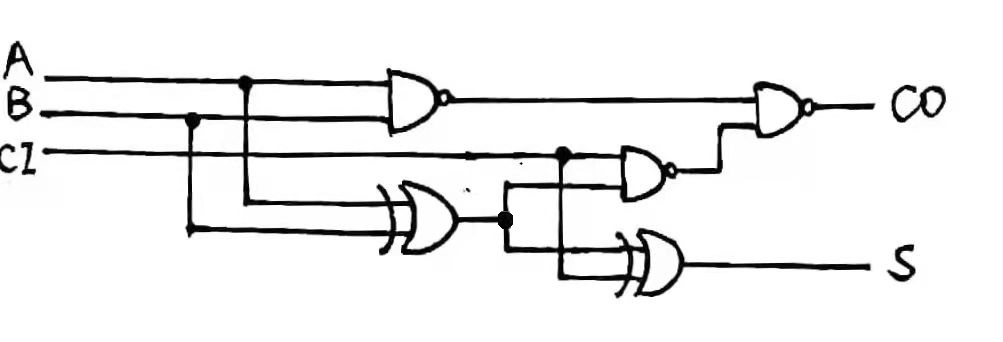
\includegraphics[scale=0.3]{1.jpg}
\end{center}\end{figure}
我们可以将其封装为一个整体,如下图所示
\begin{figure}[H]\begin{center}
    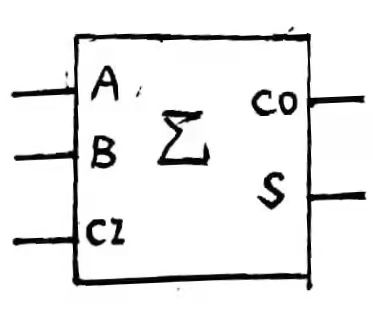
\includegraphics[scale=0.3]{2.jpg}
\end{center}\end{figure}

\subsubsection{二位全加器}
我们将两位二进制数分为高位和低位,低位相加时,用一个一位全加器计算$A_0$与$B_0$的和,结果为$S_0$. 低位的进位输出$CO_0$作为高位的进位输入$CI_1$,再将$A_1$和$B_1$相加,结果为$S_1$;进位$CO_1$作为第三位输出$S_2$. 因此,二位全加器可以用两个一位全加器串联达到运算目的.\par
逻辑式可以写作:
\[S_0 = A_0\oplus B_0 \oplus CI_0\]
\[CO_0 = (((A_0\oplus B_0)CI_0)'(A_0B_0)')'\]
\[S_1 = A_1\oplus B_1 \oplus CI_1\]
\[CO_1 = (((A_1\oplus B_1)CI_1)'(A_1B_1)')'\]
电路图如下
\begin{figure}[H]\begin{center}
    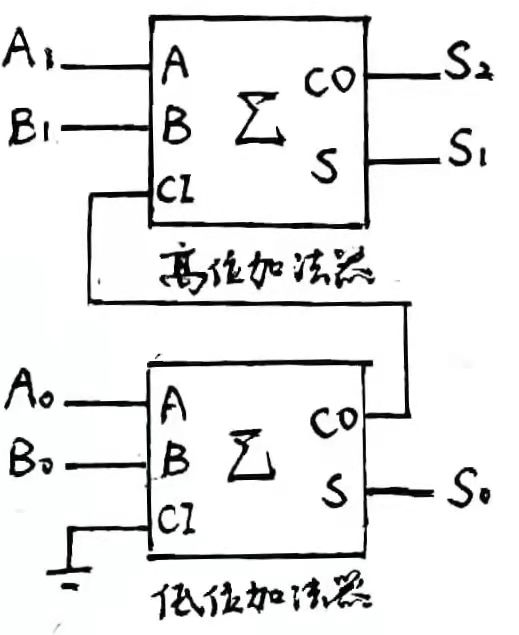
\includegraphics[scale=0.3]{3.jpg}
\end{center}\end{figure}
因此,两个二位二进制数加和结果可以表示为$(\overline{CO_1S_1S_0})_2$. 
到此为止,我们已经完成了实验的基本内容,设计出了两位二进制数加法器.

\subsubsection{用补码显示的二位减法器}
我们用一个二进制输入M表示加减,M=0表示加法,M=1表示减法. \par
进行减法运算时M=1,我们只需要将B换算成补码,并将A与B的补码相加,即可得到A-B的补码. 我们先考虑如何将B转化为补码形式. 转化为补码时,将B的每一位取反,并且在最终结果上加1,考虑到我们已经设计出了两位加法器,因此将A的末两位和B的末两位按位取反后相加,并且令进位输入$CI_0=1=M$以表示求补码时按位取反后加的1. 利用二位全加器计算出的$S_1S_0$即为计算结果的后两位,而最高位符号位结果即为$CO_1\oplus 1$(取反).\par
加法运算时M=0,B的末两位不需要按位取反,进位输入$CI_0=0=M$,计算出的最高位符号位结果为$CO_1$. \par
在这里,我们可以将加法器输入值$BI_0$与原值$B_0$做比较,列出真值表:

因此,我们可以将加法和减法电路统一起来,设计的电路图如下:
\begin{table}[H]
    \label{biao}
    \begin{center}
    \begin{tabular}{p{4em}<{\centering}|p{4em}<{\centering}|p{4em}<{\centering}|p{12em}<{\centering}}
        \hline\hline
        M&$B_0$&$BI_0$&含义\\
        \hline
        0&0&0&加法运算,不取反\\
        \hline
        0&1&1&加法运算,取反\\
        \hline
        1&0&1&减法运算,取反\\
        \hline
        1&1&0&减法运算,取反\\
        \hline
    \end{tabular}
\end{center}
\end{table}
因此有$BI_0=M'B_0+MB_0=M\oplus B_0$. 类似地,$BI_1=M\oplus B_0$;结果最高位$S_2=M\oplus CO_1$.
以此,我们就可以利用二位全加器进行减法运算了. 电路图如下所示:
\begin{figure}[H]\begin{center}
    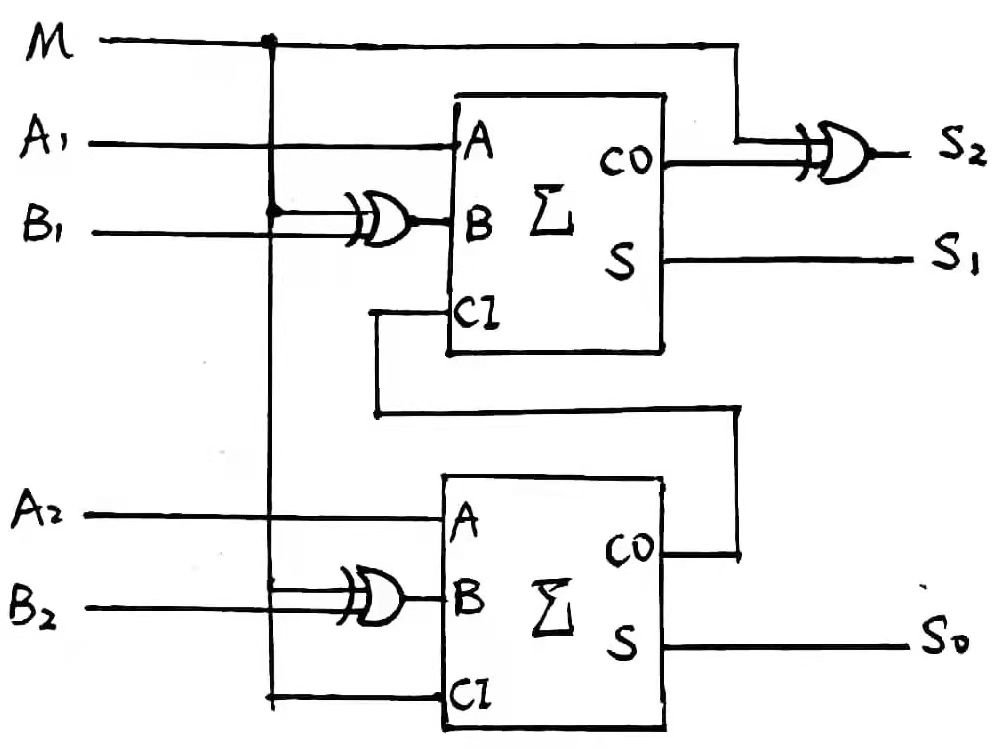
\includegraphics[scale=0.25]{4.jpg}
\end{center}\end{figure}

\subsection{电路实物图}
\begin{figure}[H]\centering
    {
        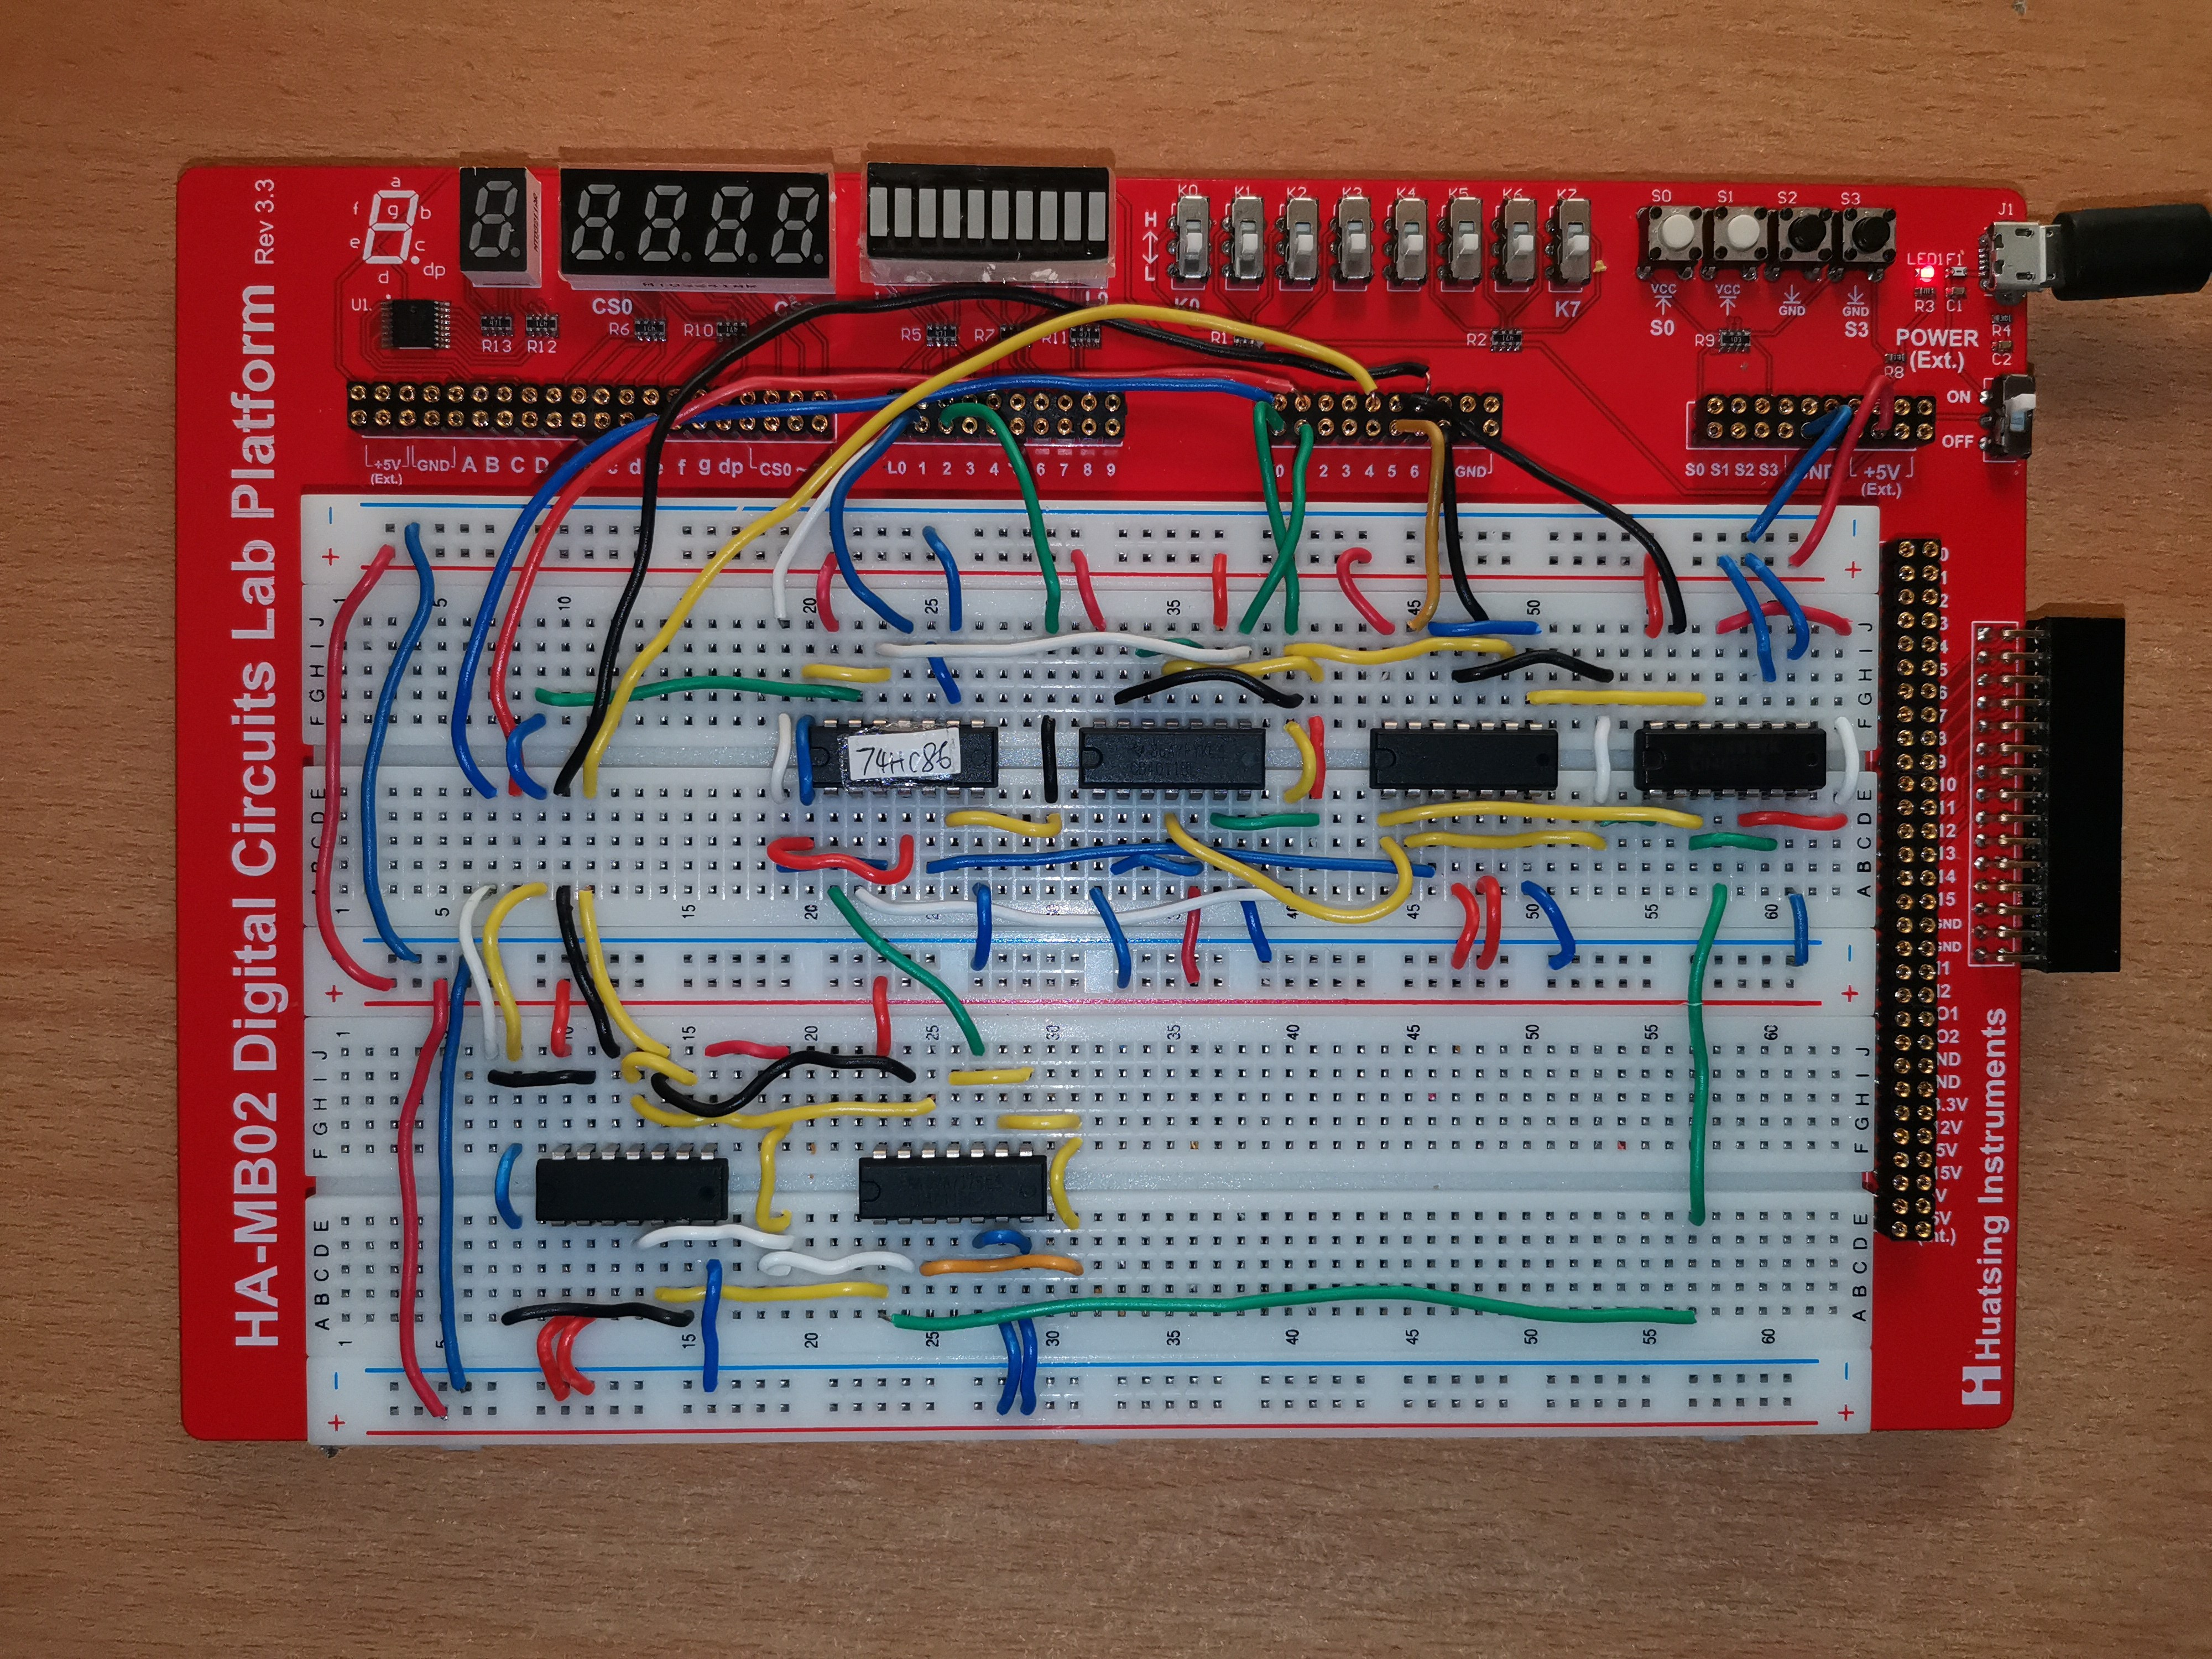
\includegraphics[scale=0.08]{10.jpg}
        \caption{用补码显示的二位减法器}
    }
\end{figure}\par
\vspace{-2em}

\subsection{功能展示}
\begin{figure}[H]\centering
    {
    \newgeometry{a4paper,left=3cm,right=0cm}
    \vspace{-1em}
    \subfigcapskip=-10pt
    \subfigure[0+1]{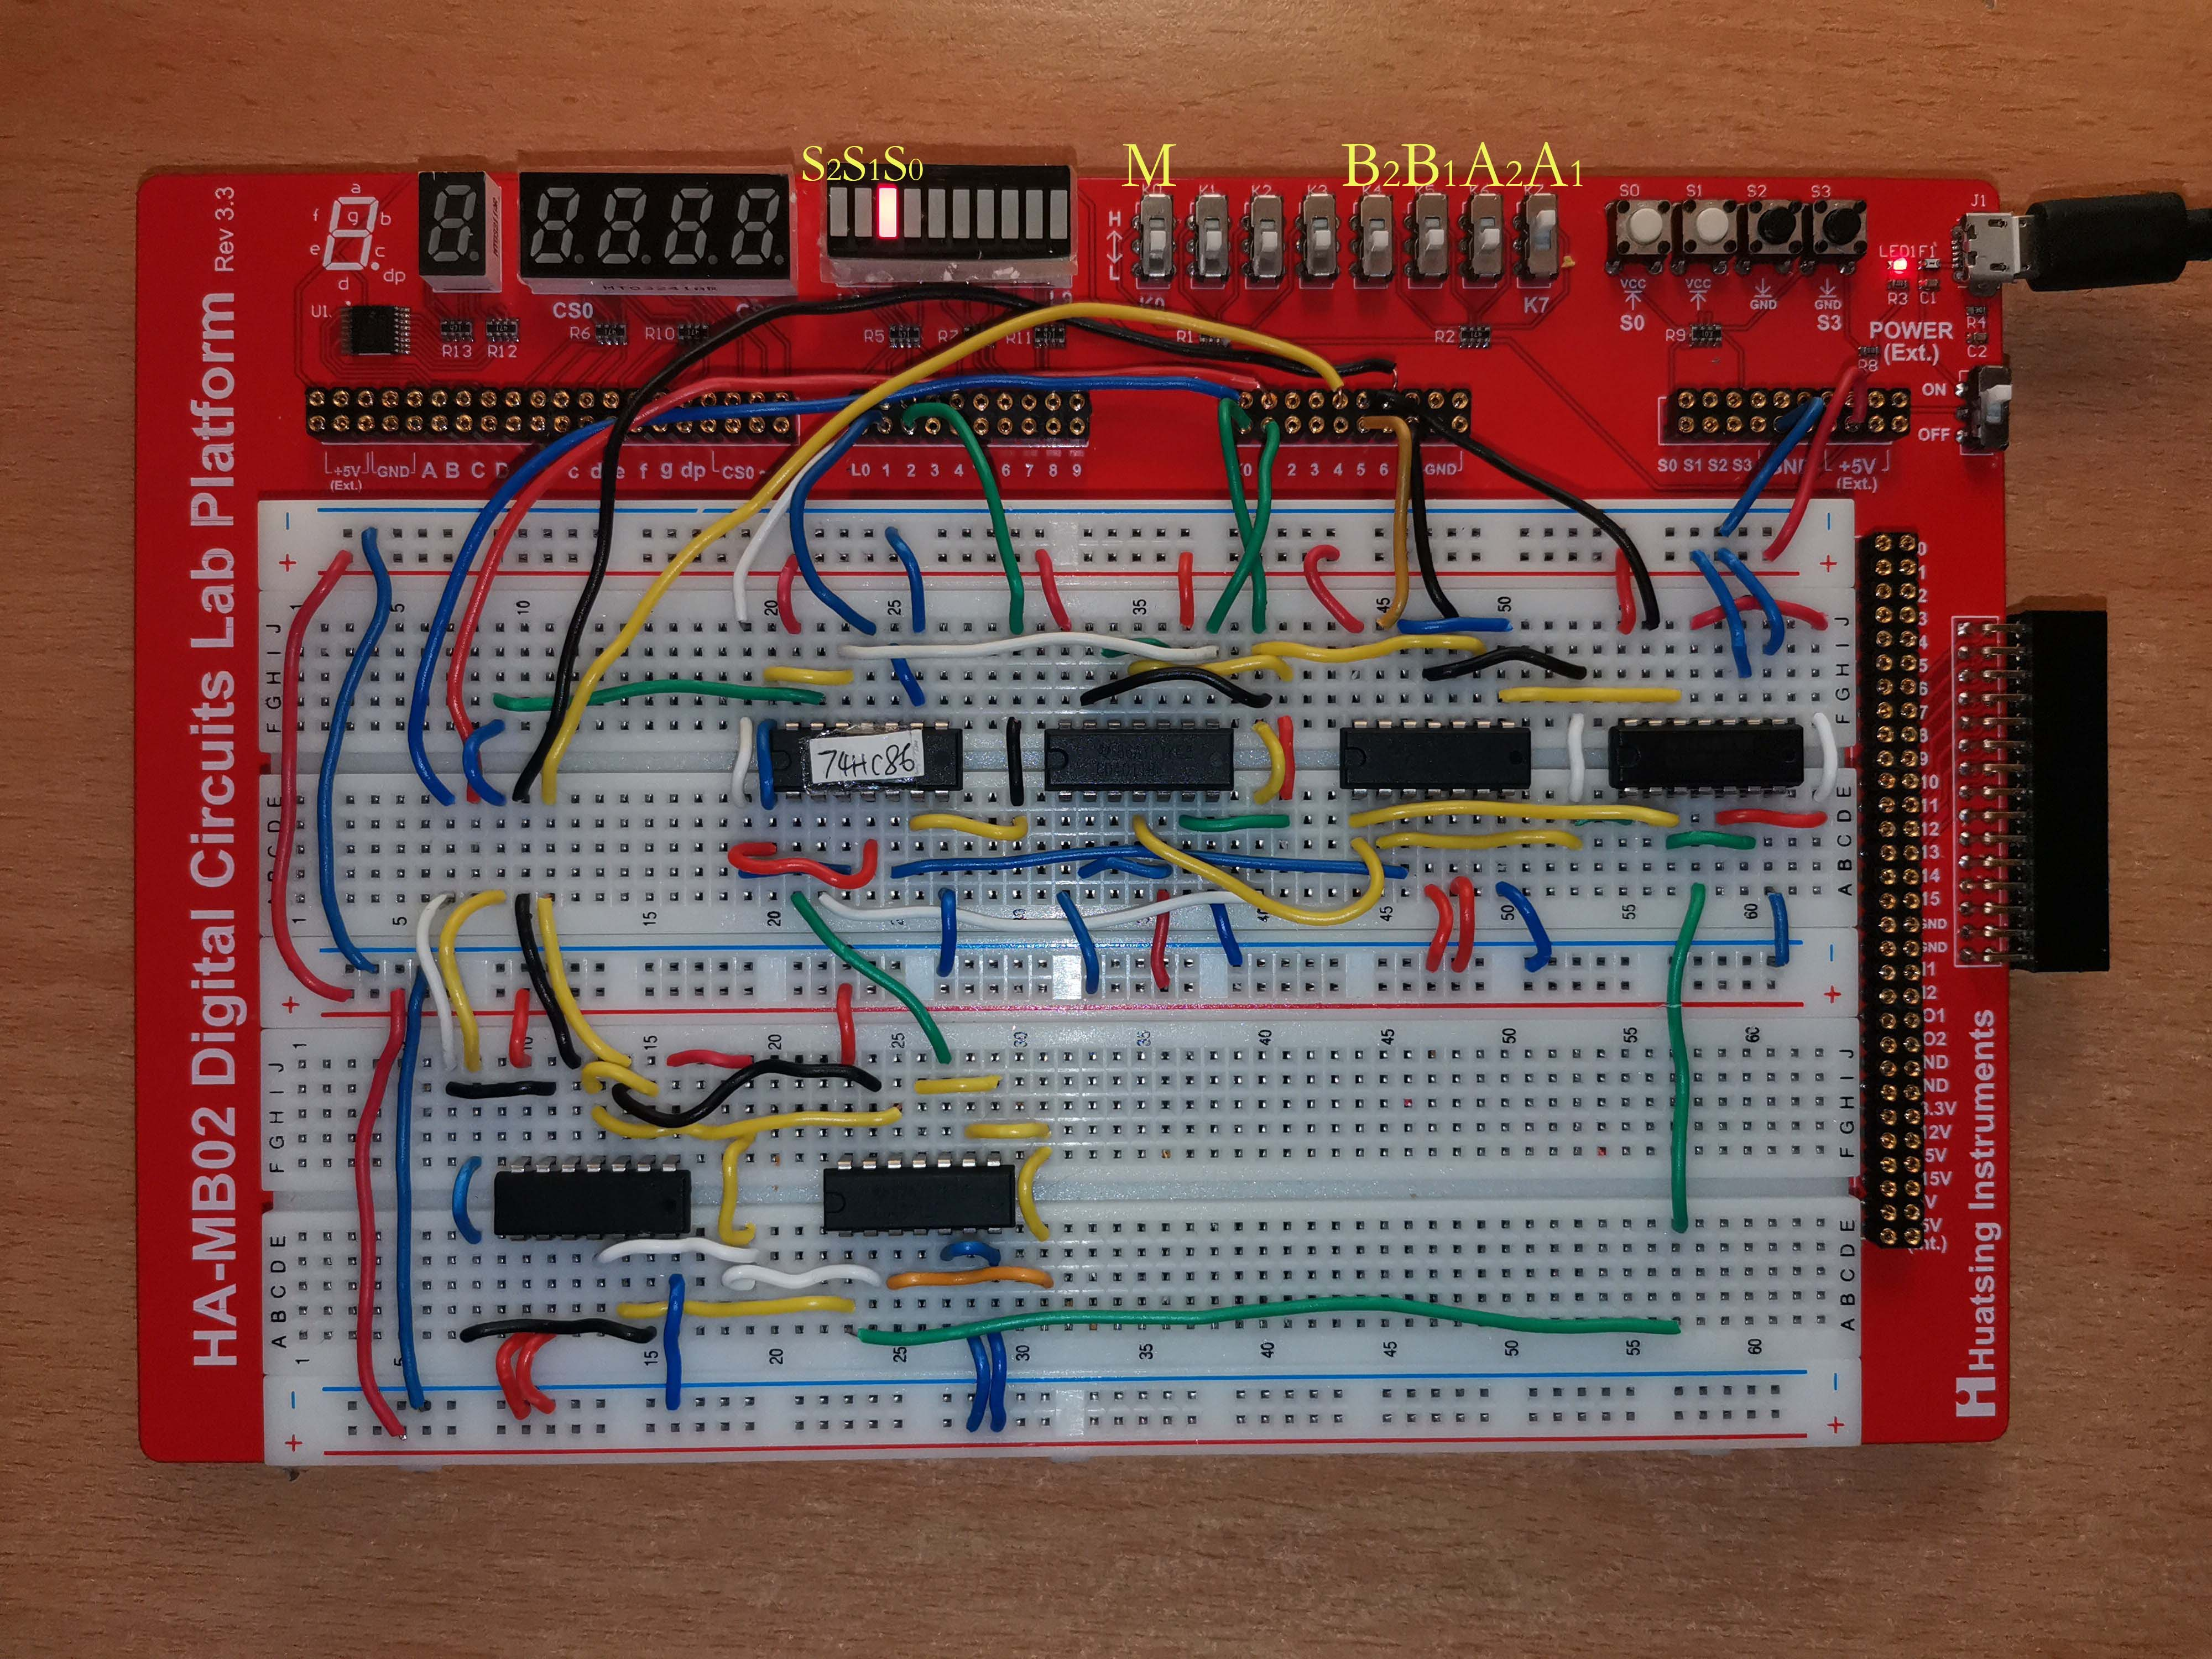
\includegraphics[scale=0.04]{0+1.jpg}}\hspace{0.3mm}
    \subfigure[1+1]{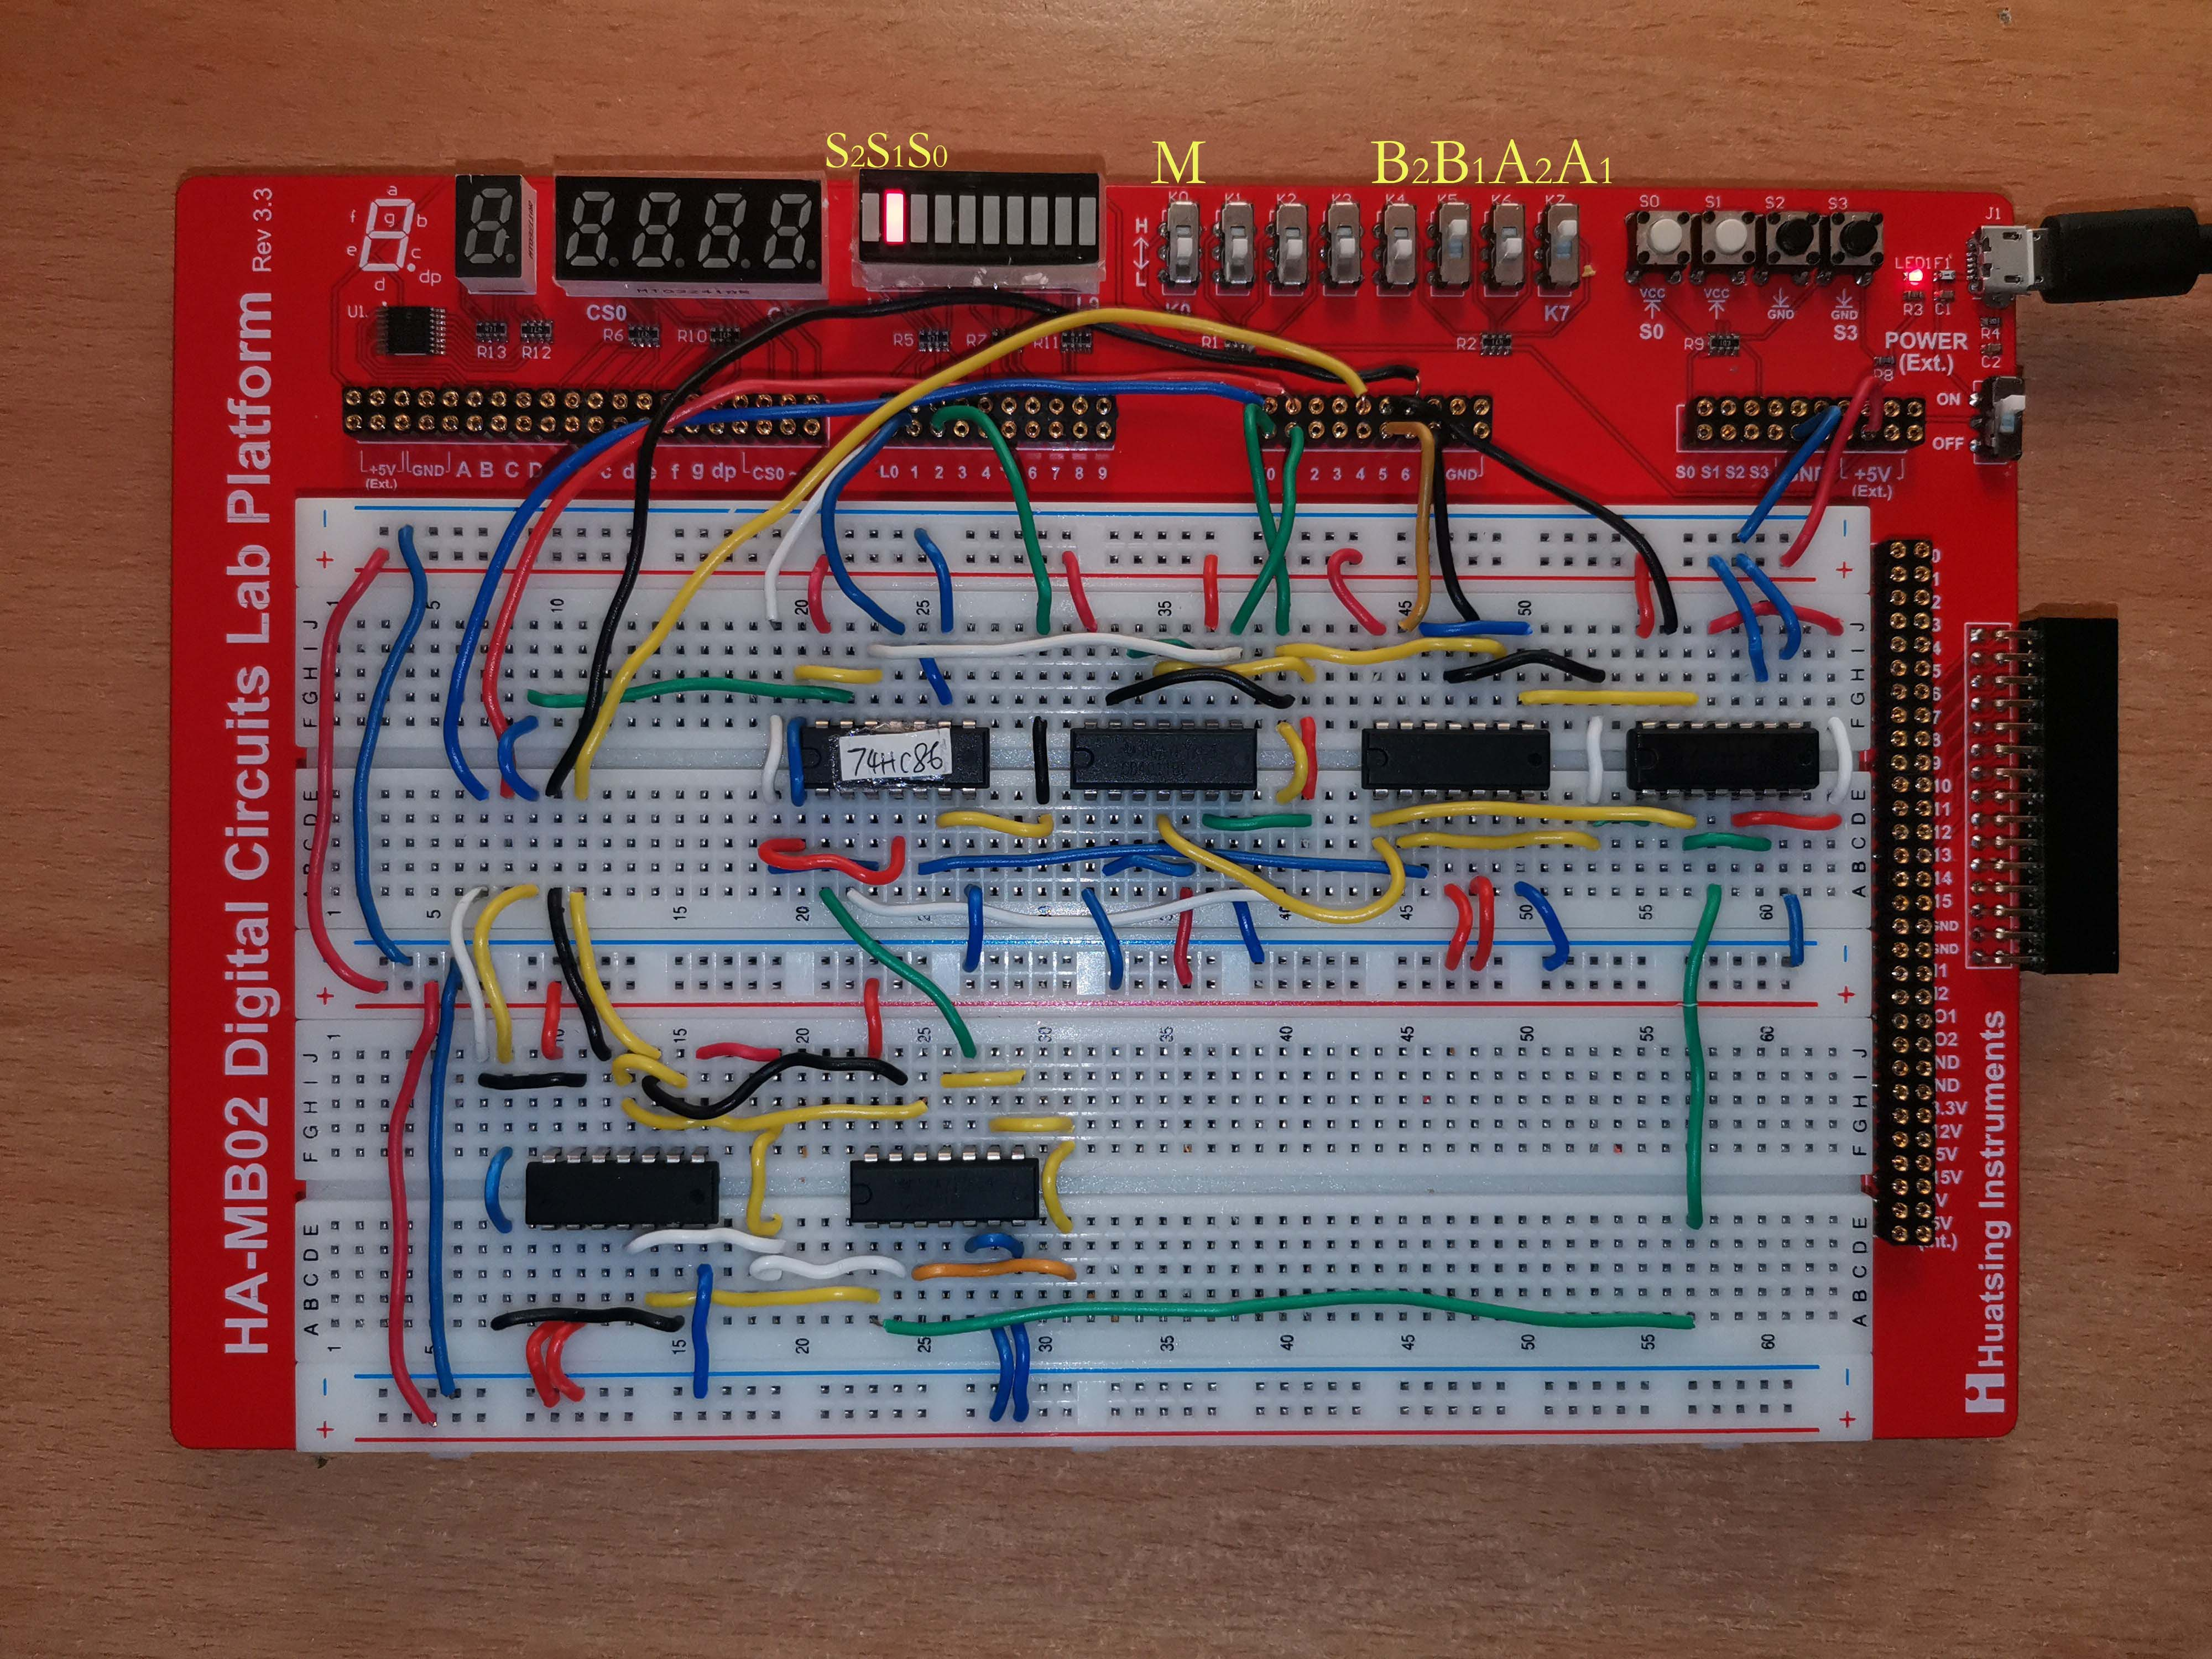
\includegraphics[scale=0.04]{1+1.jpg}}\hspace{0.3mm}    
    \subfigure[1+2]{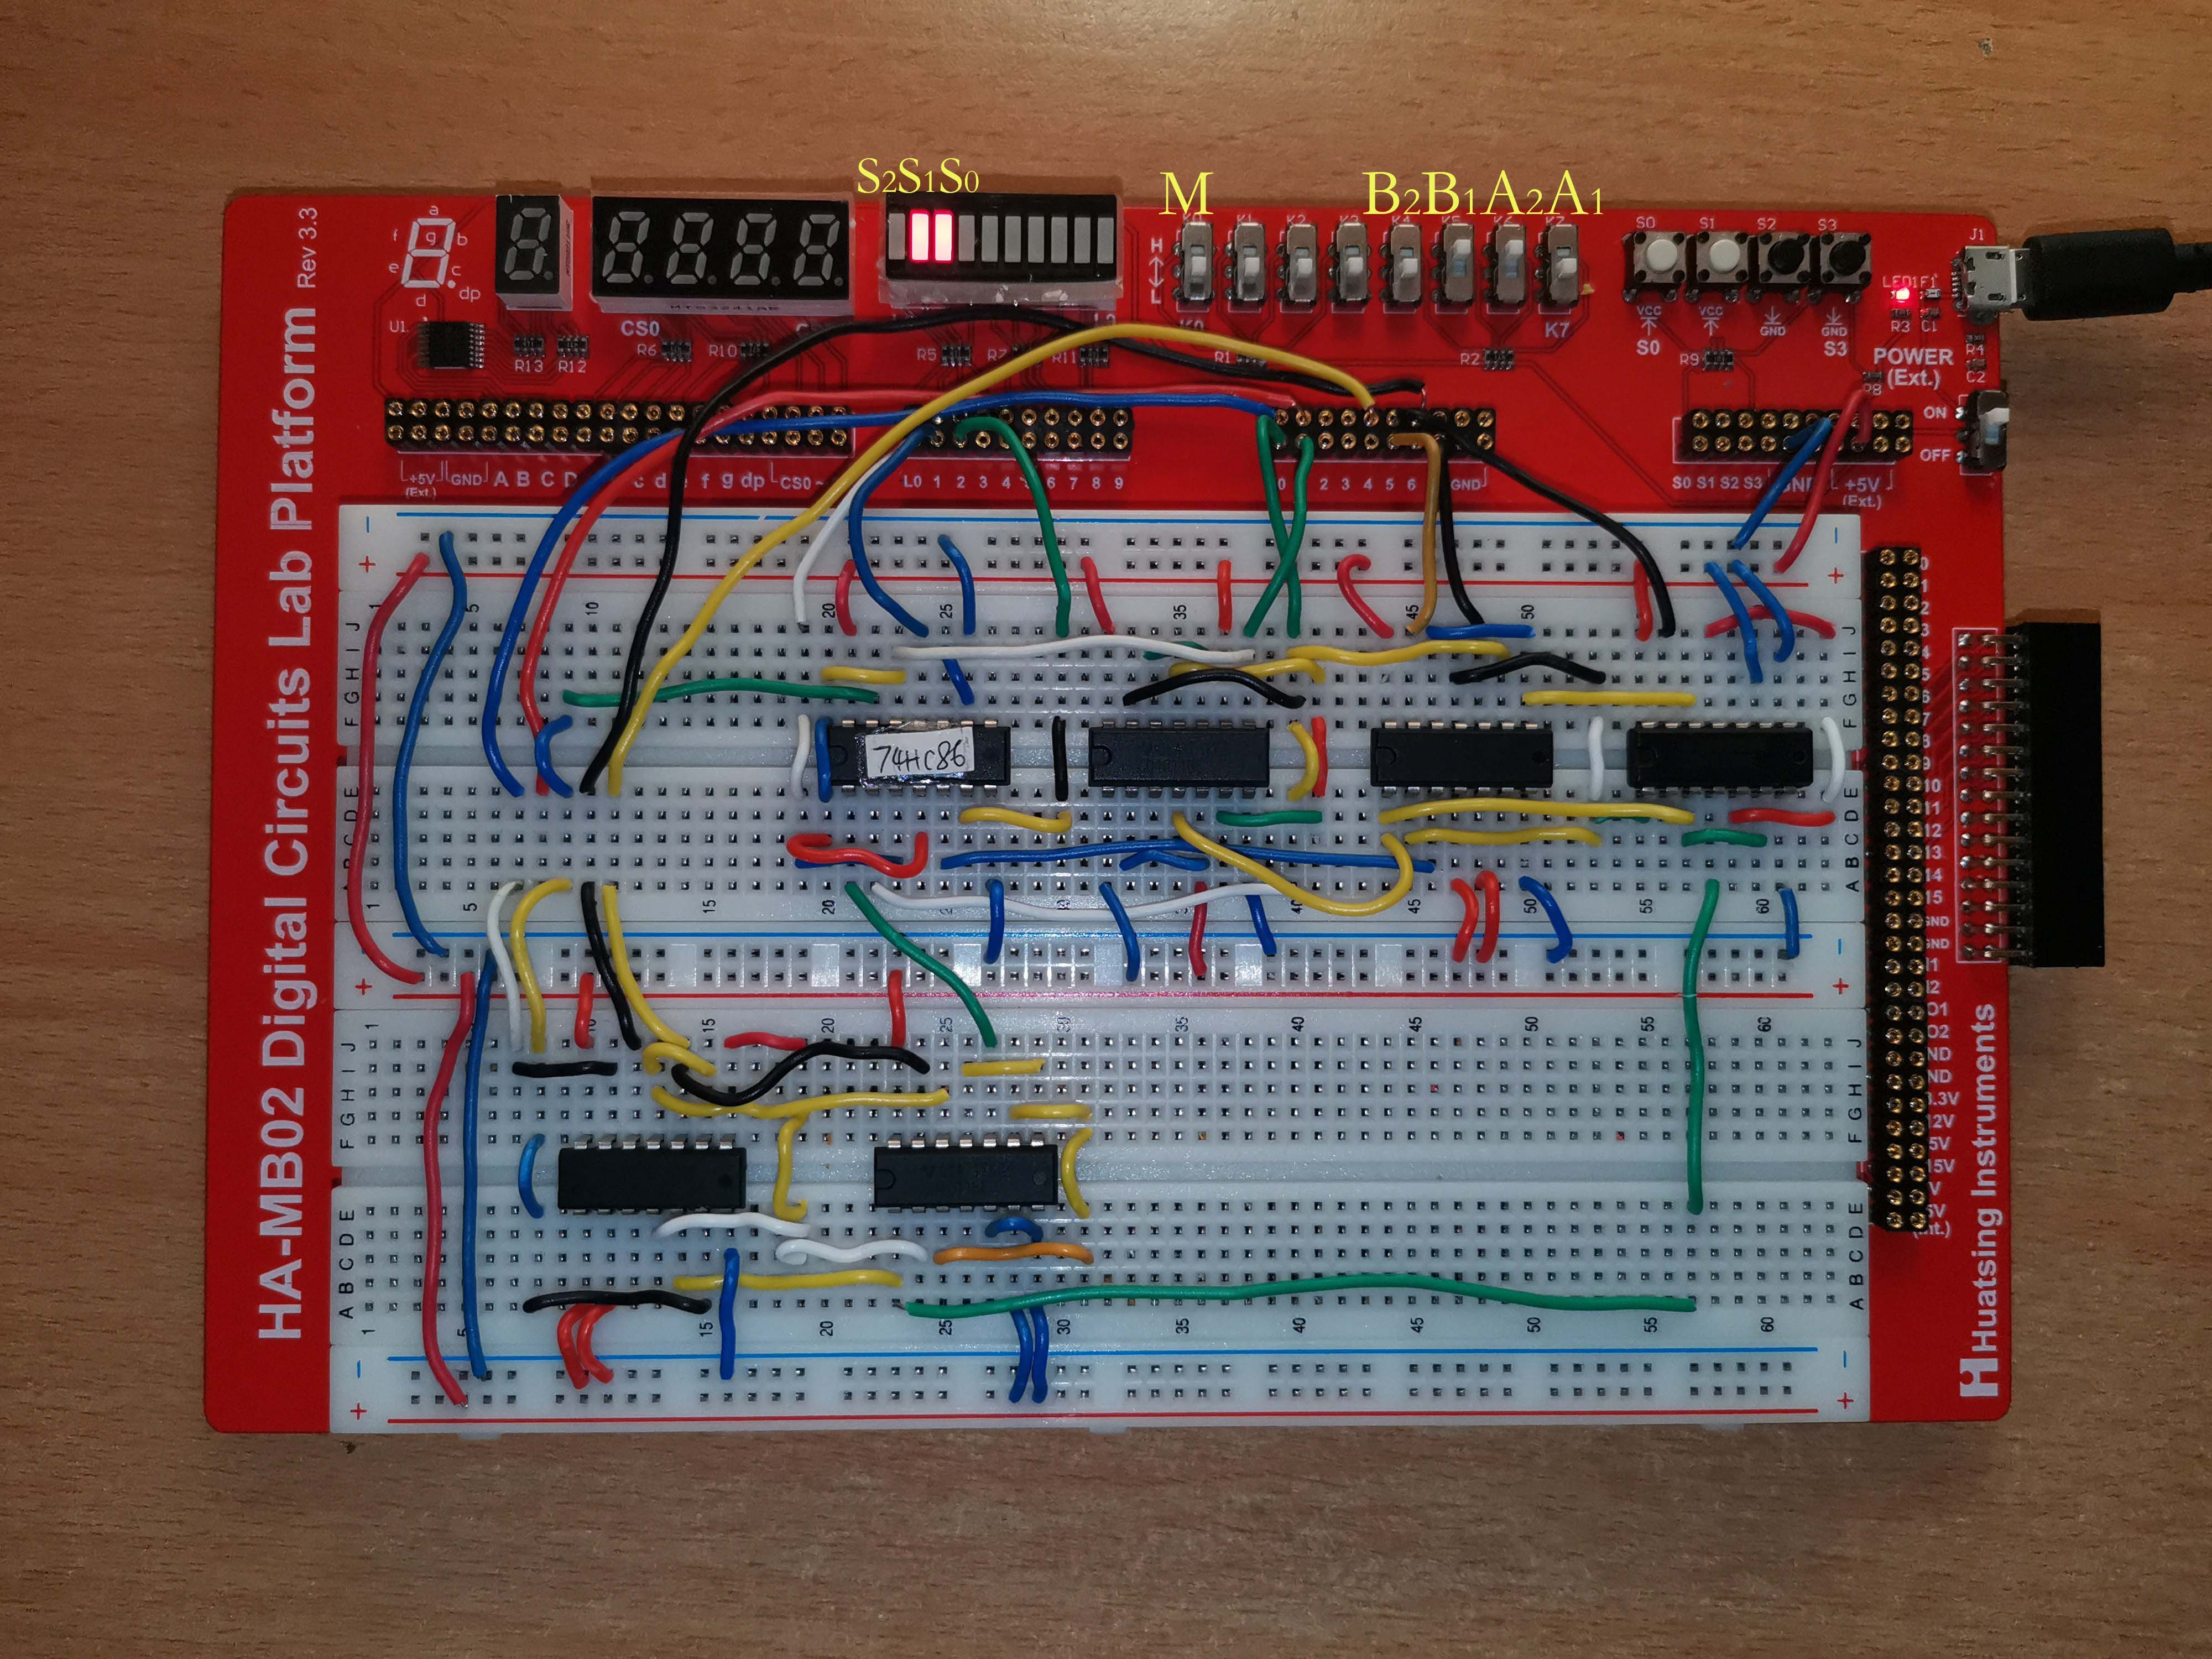
\includegraphics[scale=0.04]{1+2.jpg}}\hspace{0.3mm}
    \subfigure[1+3]{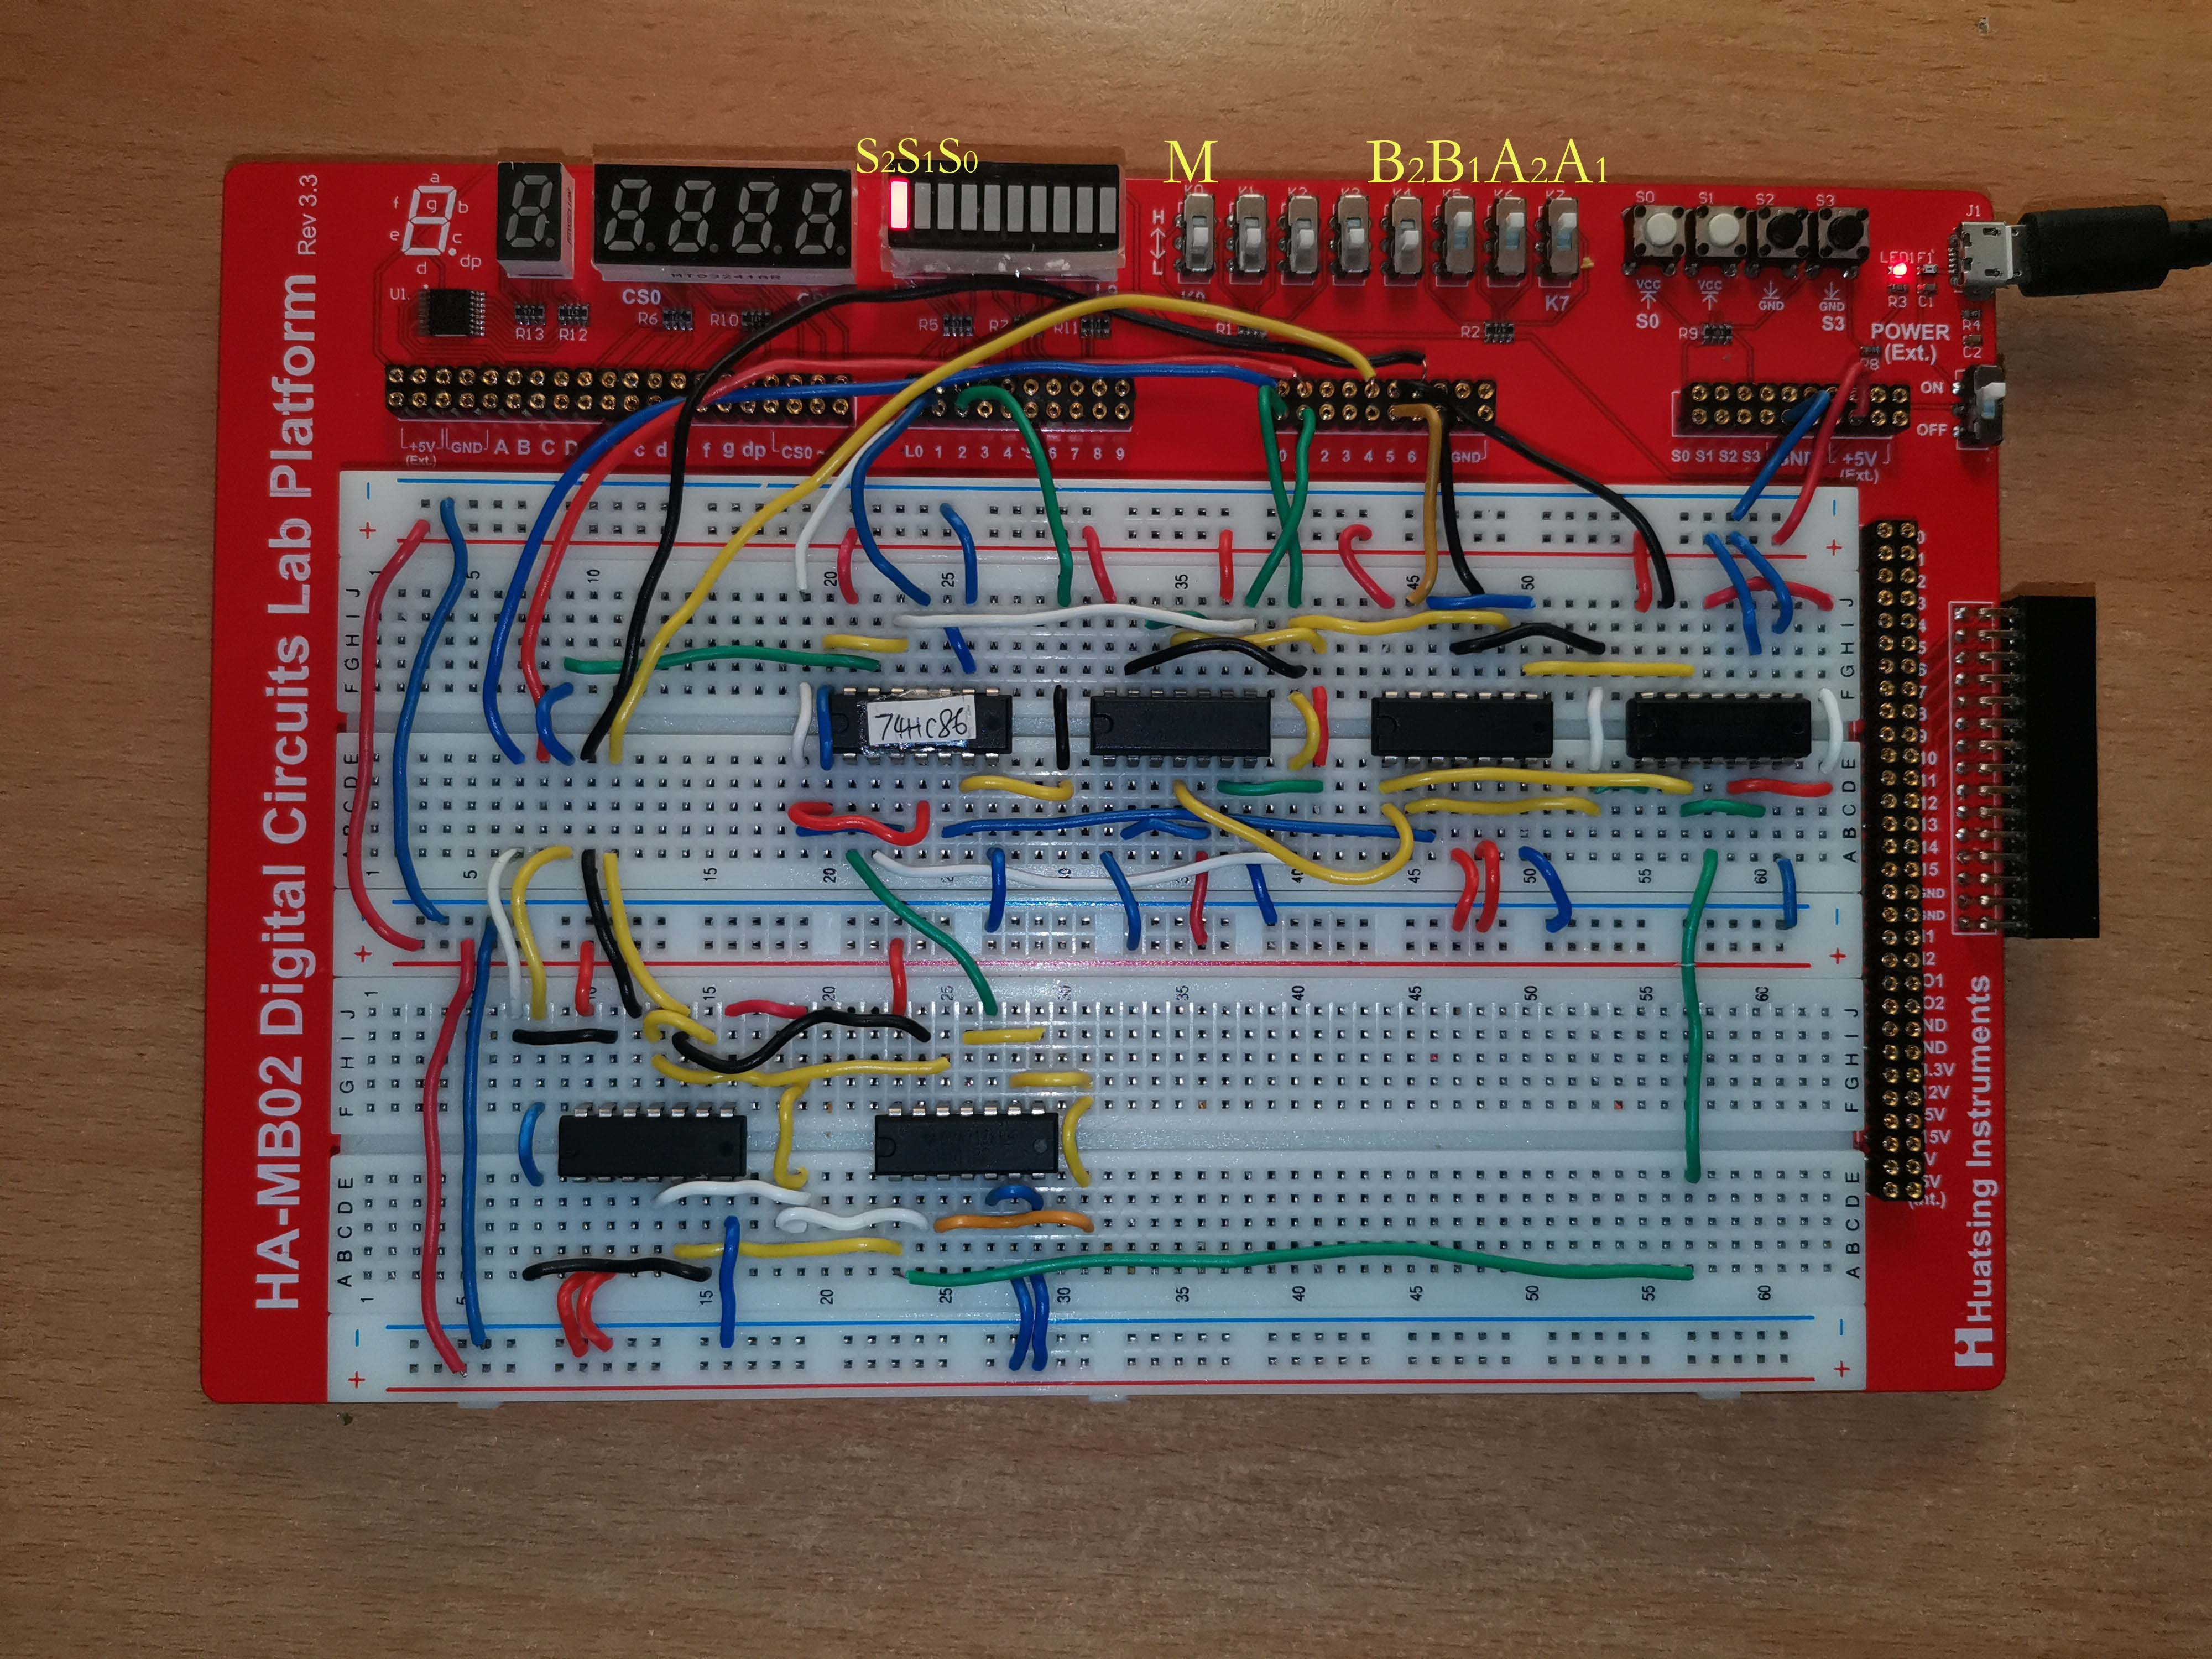
\includegraphics[scale=0.04]{1+3.jpg}}\hspace{0.3mm}
    \subfigure[2+3]{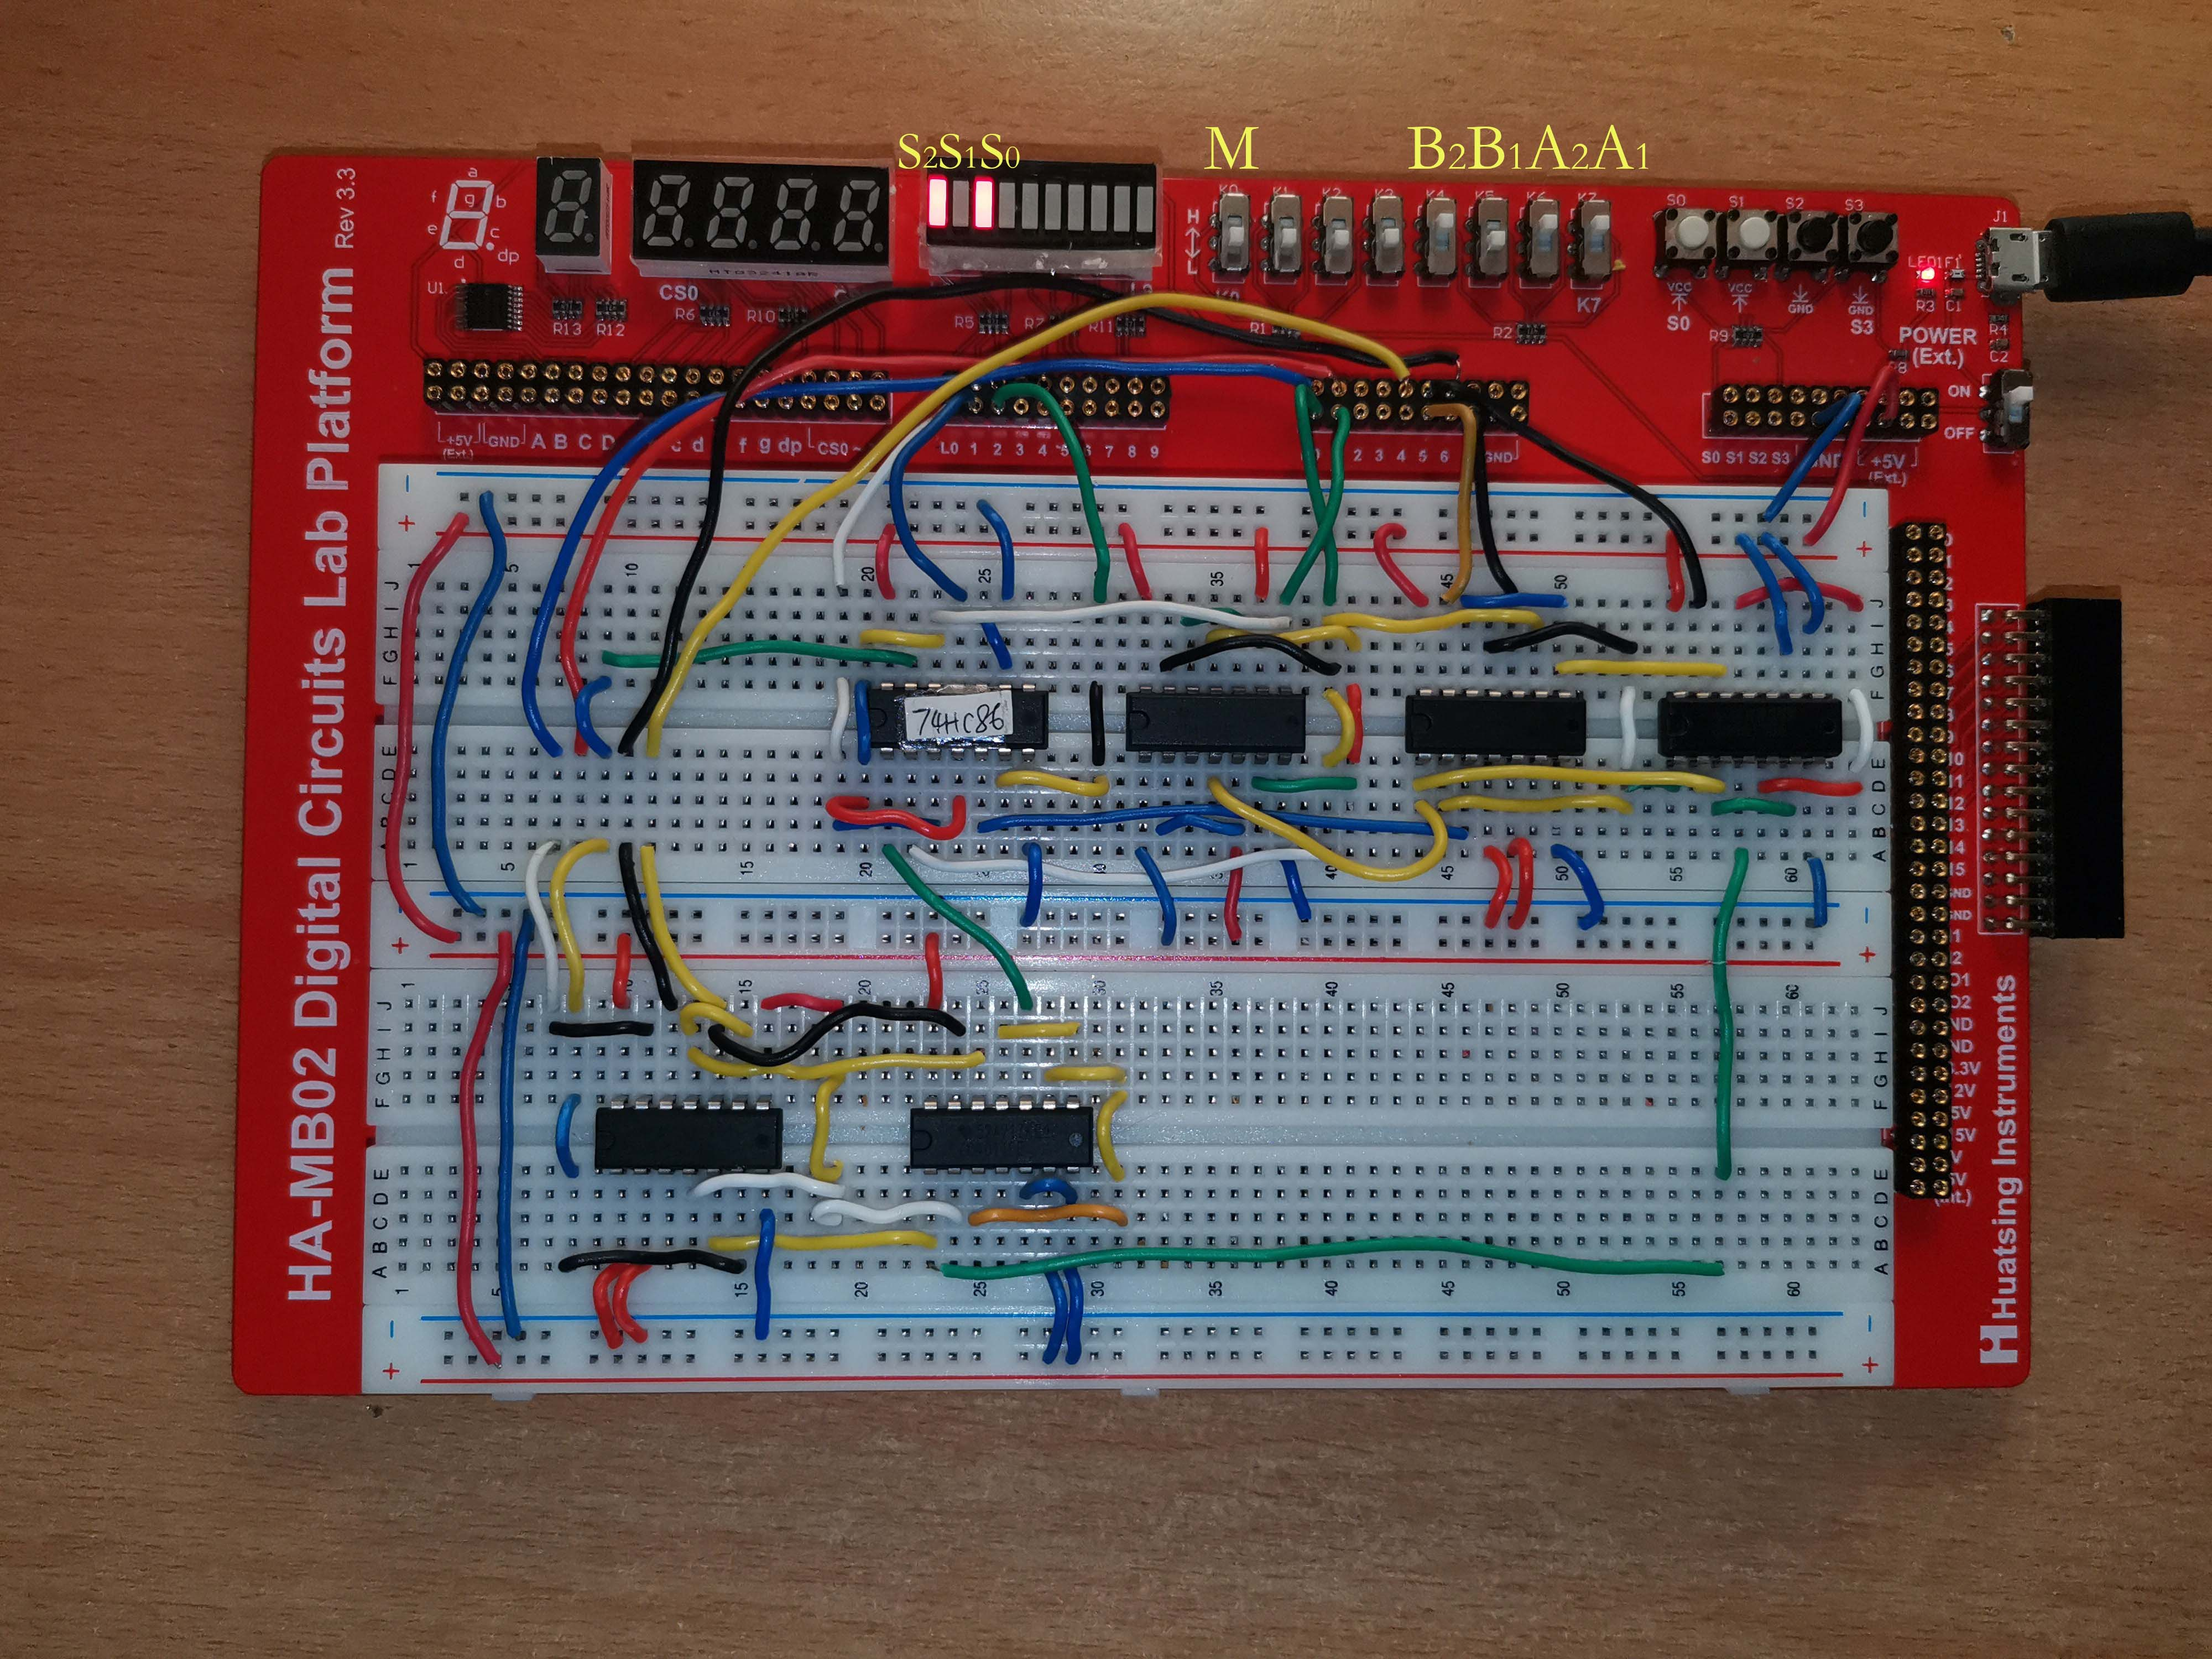
\includegraphics[scale=0.04]{2+3.jpg}}\hspace{0.3mm}
    \subfigure[3+3]{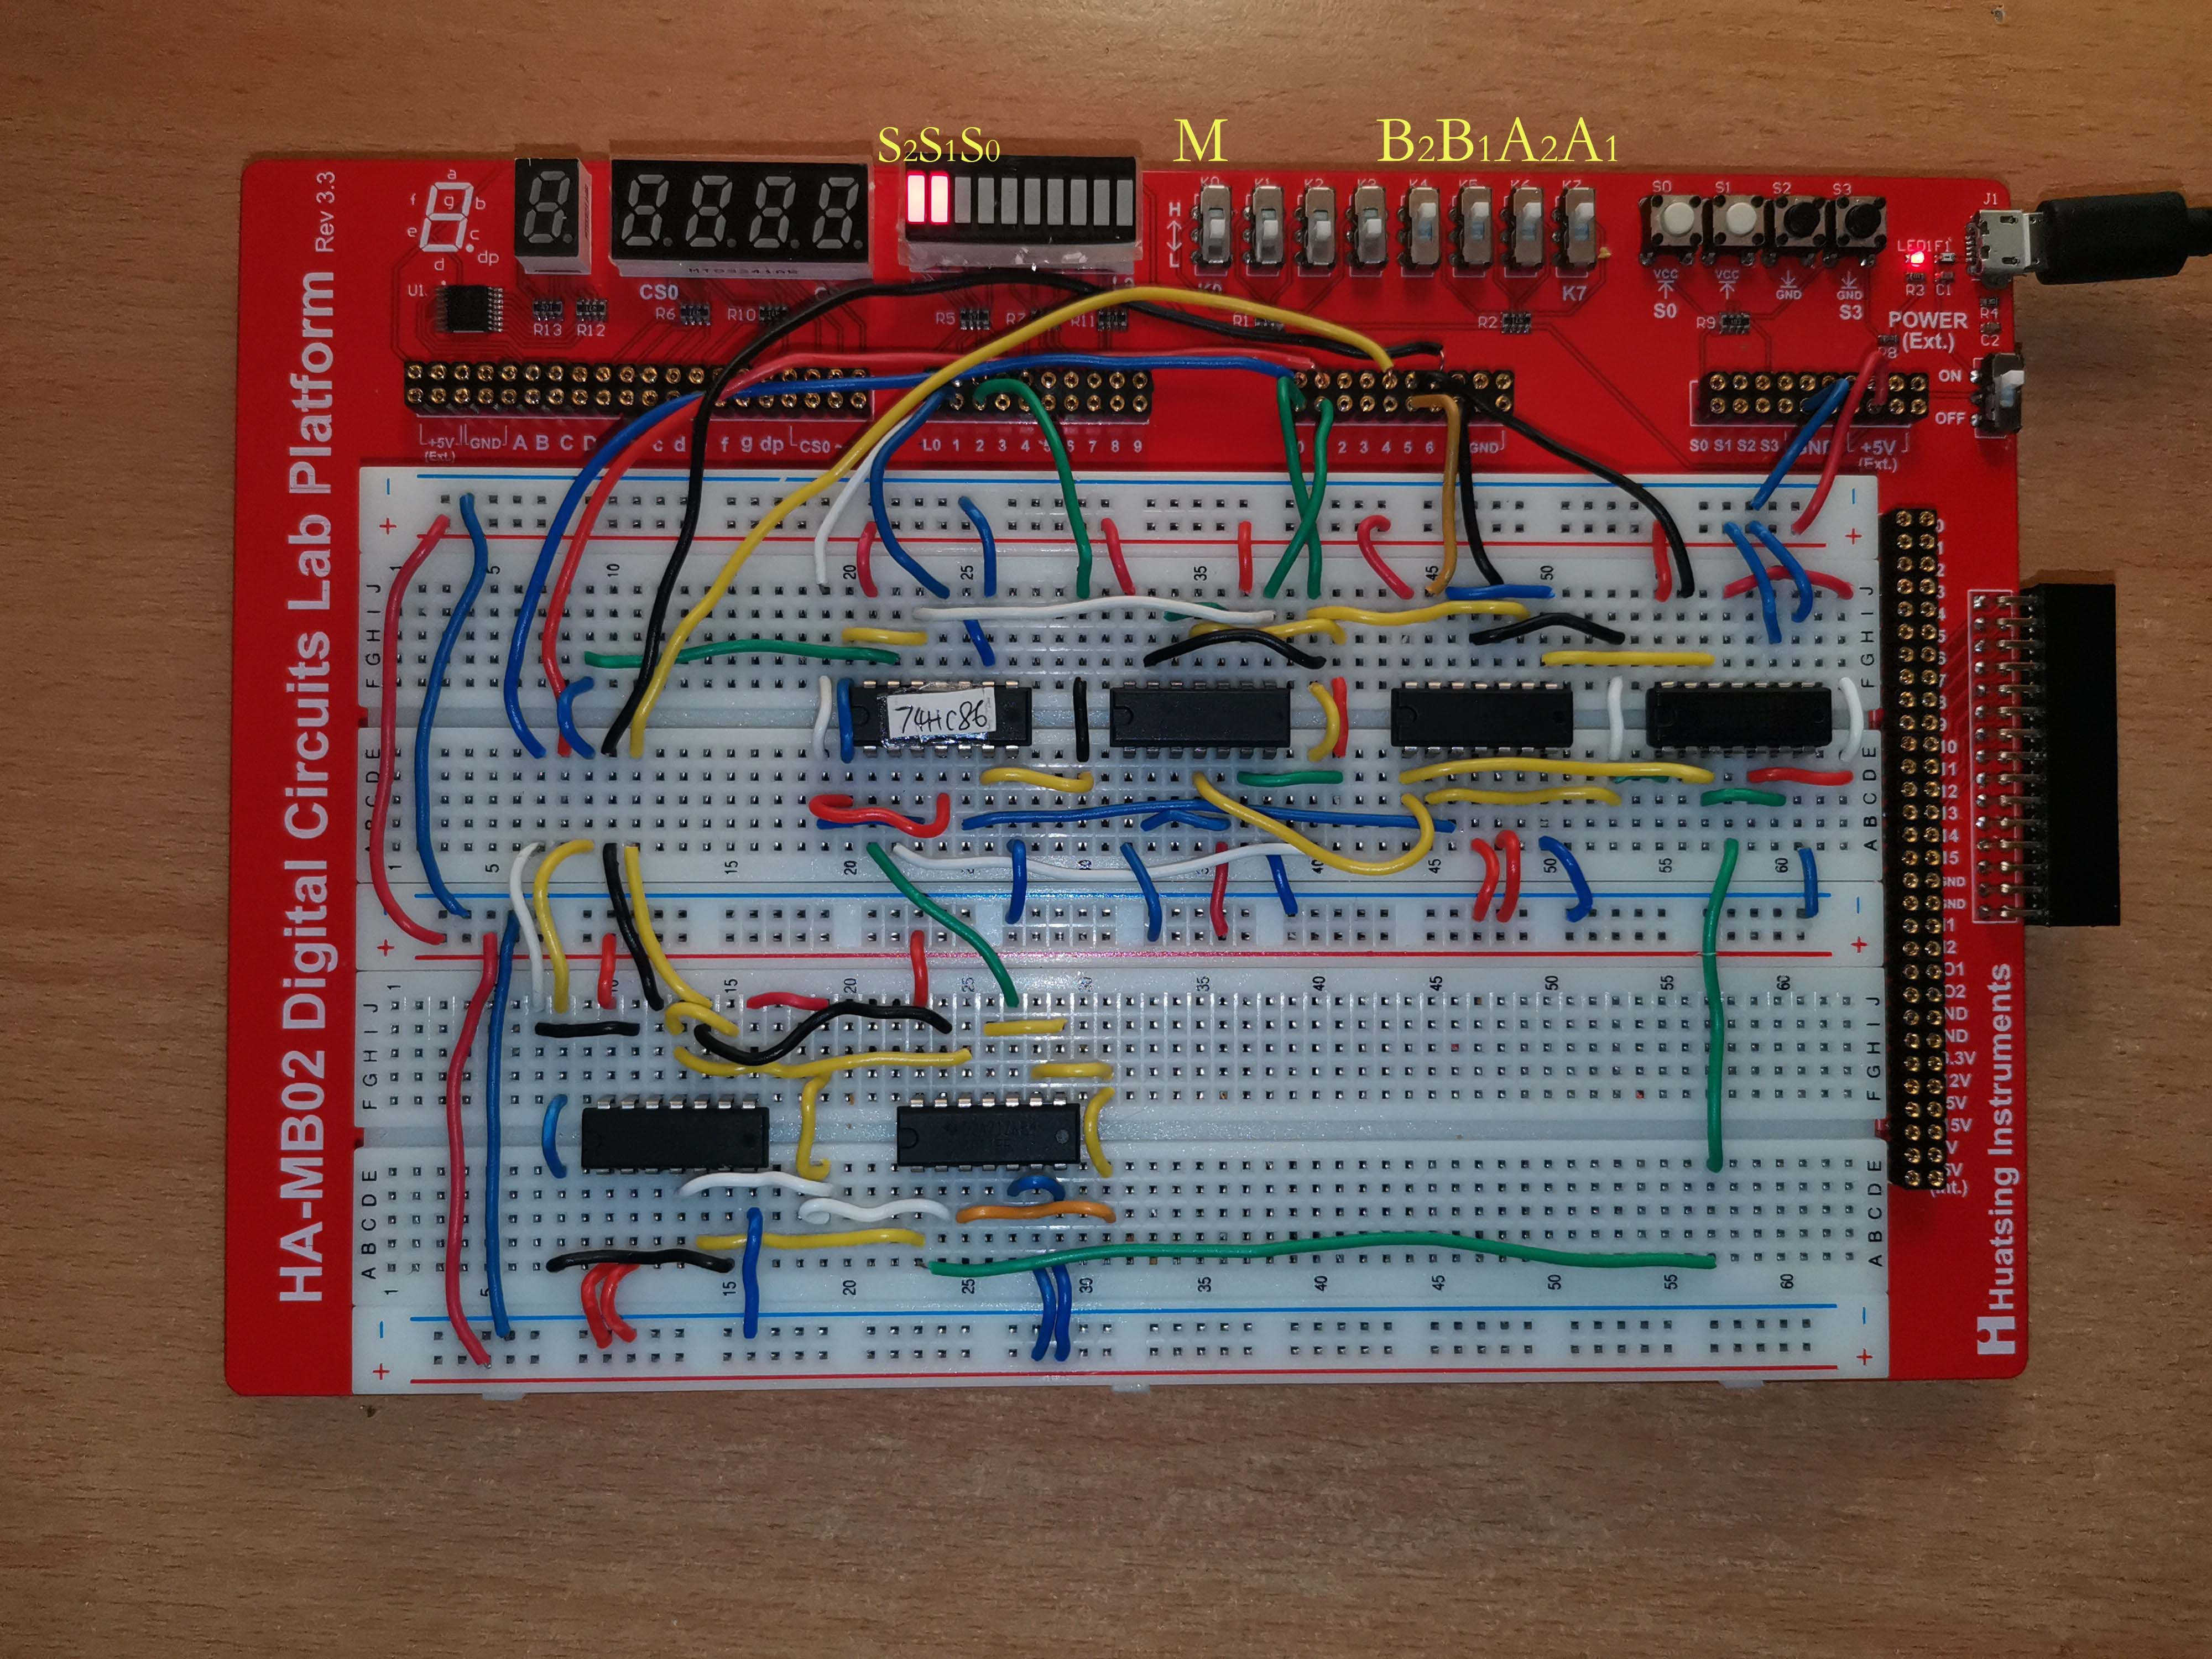
\includegraphics[scale=0.04]{3+3.jpg}}\hspace{0.3mm}
    \vspace{-1em}
    \caption{加法器}
    \restoregeometry
    }
\end{figure}\par
\vspace{-1.7em}

\begin{figure}[H]\centering
    {
    \setcounter{subfigure}{0}
    \newgeometry{a4paper,left=3cm,right=0cm}
    \vspace{-2em}
    \subfigcapskip=-10pt
    \subfigure[3-0]{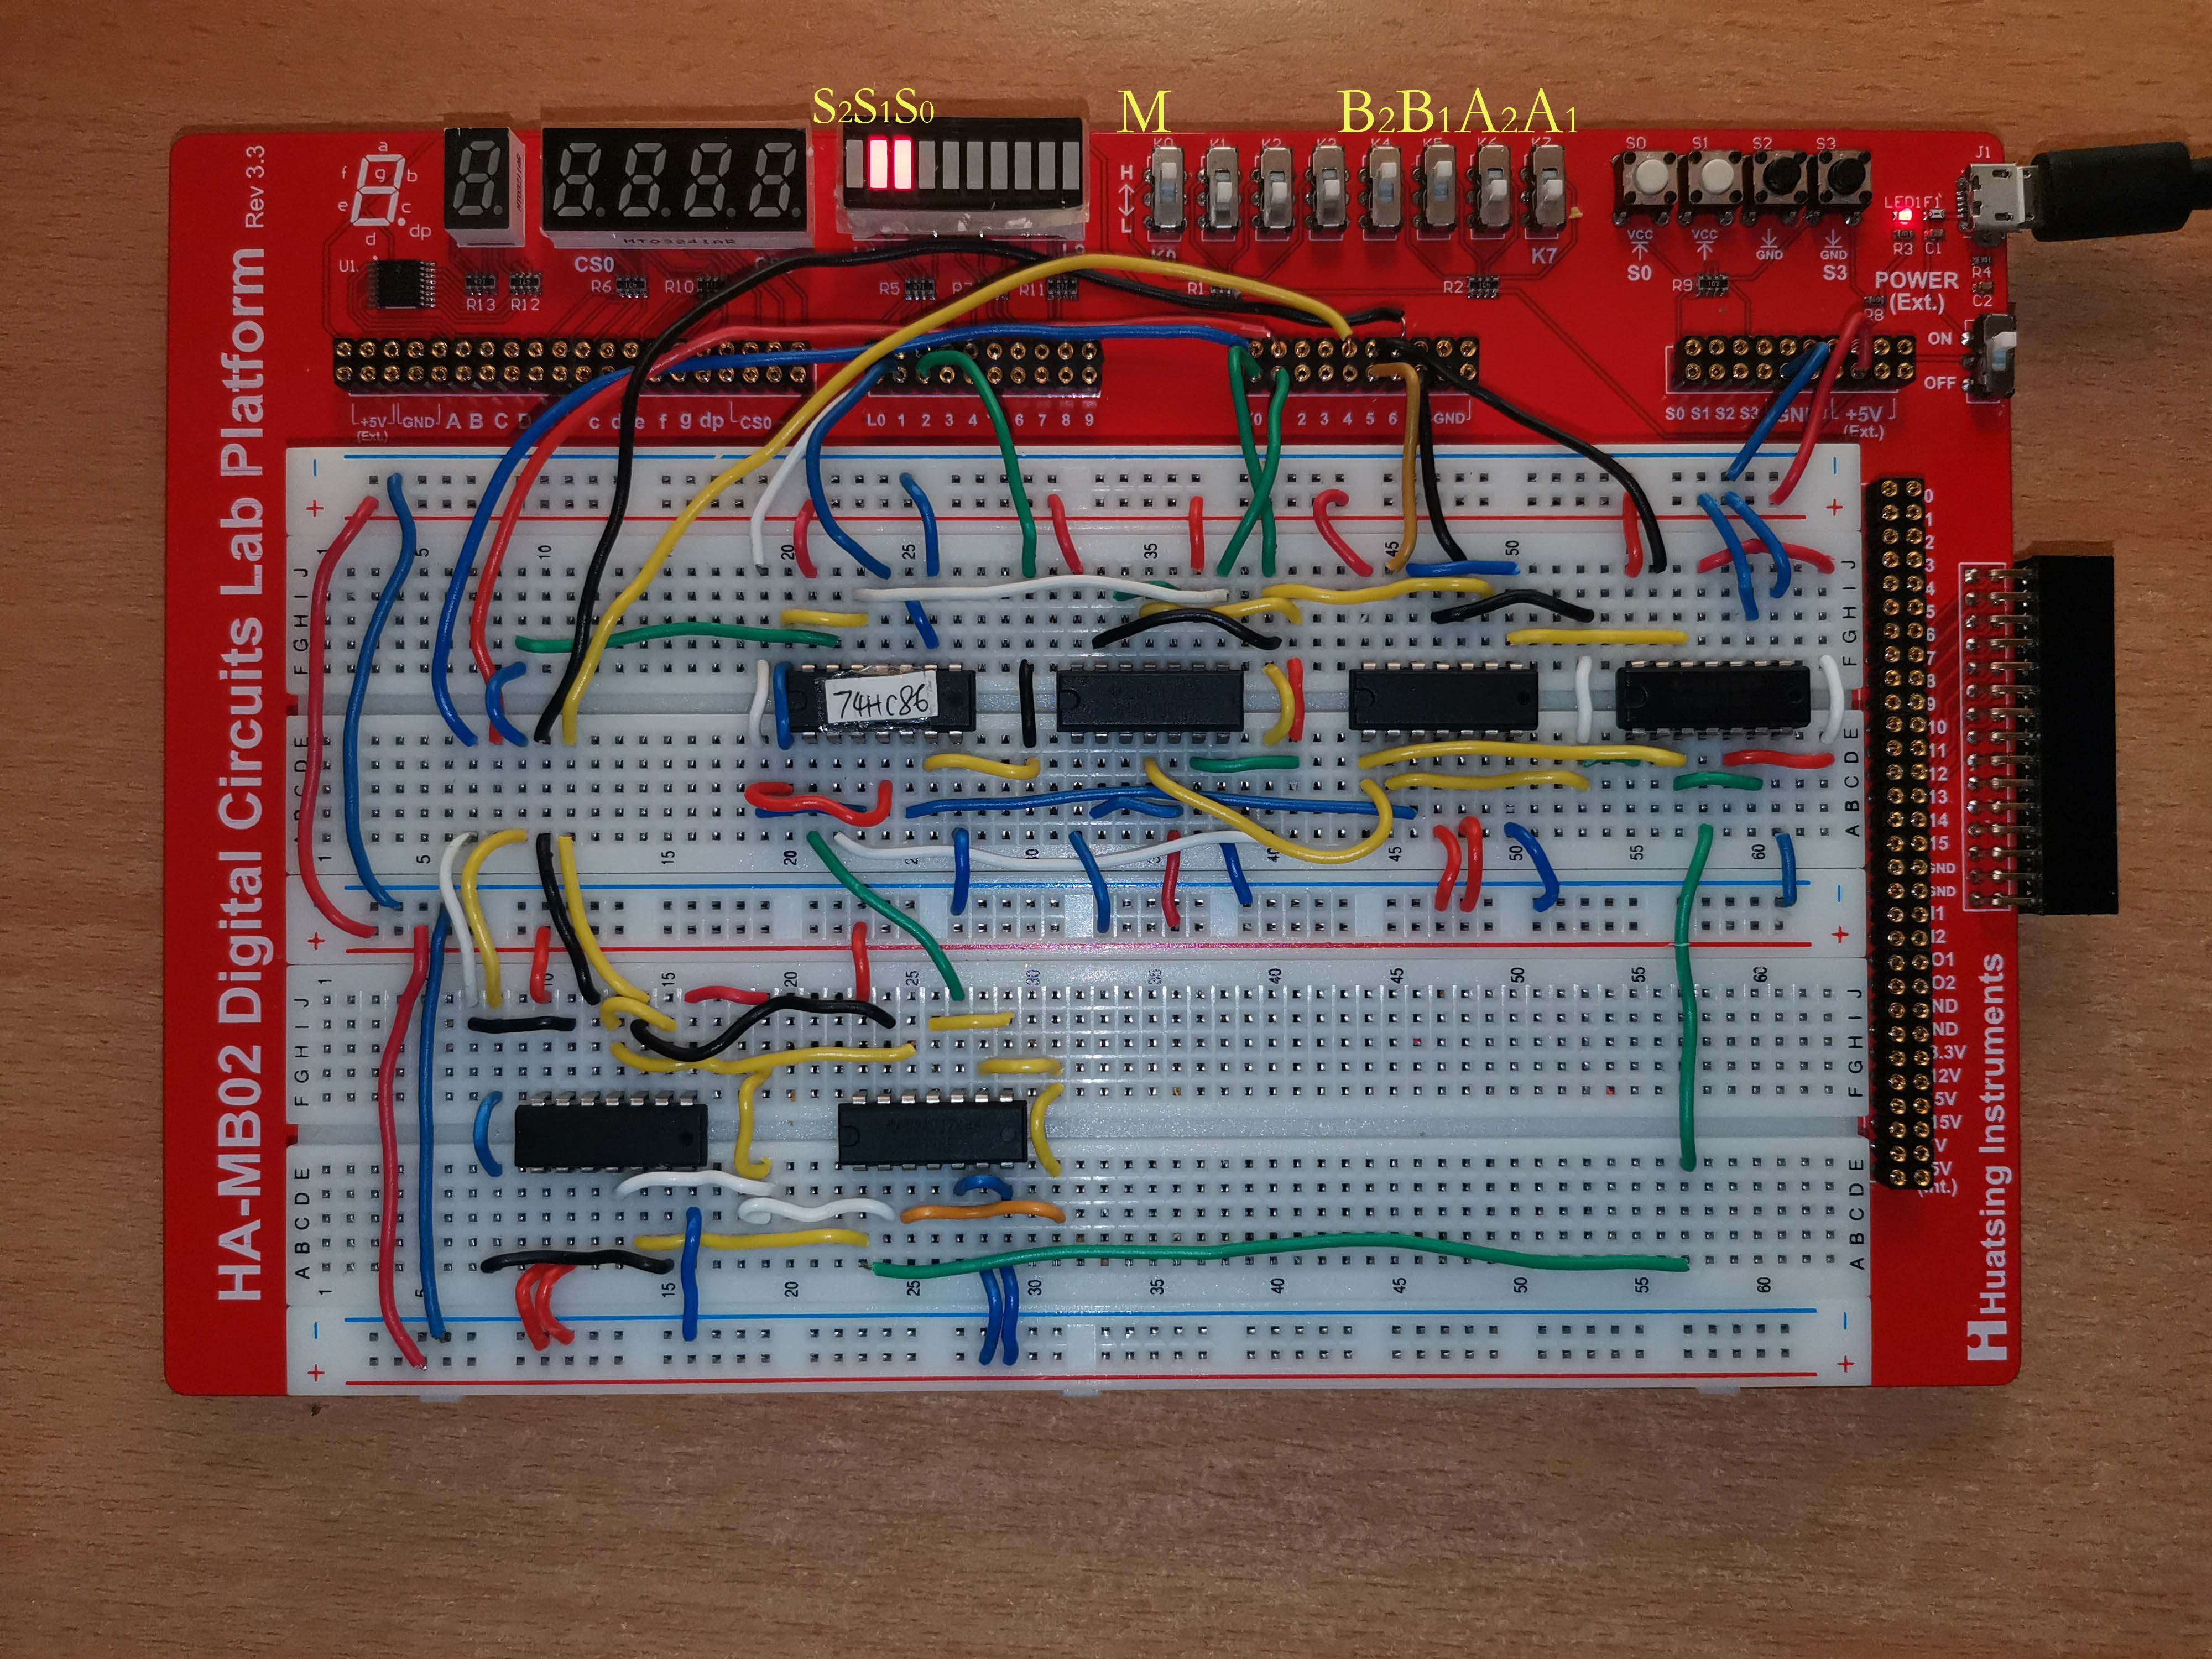
\includegraphics[scale=0.04]{3-0.jpg}}\hspace{0.3mm}
    \subfigure[3-1]{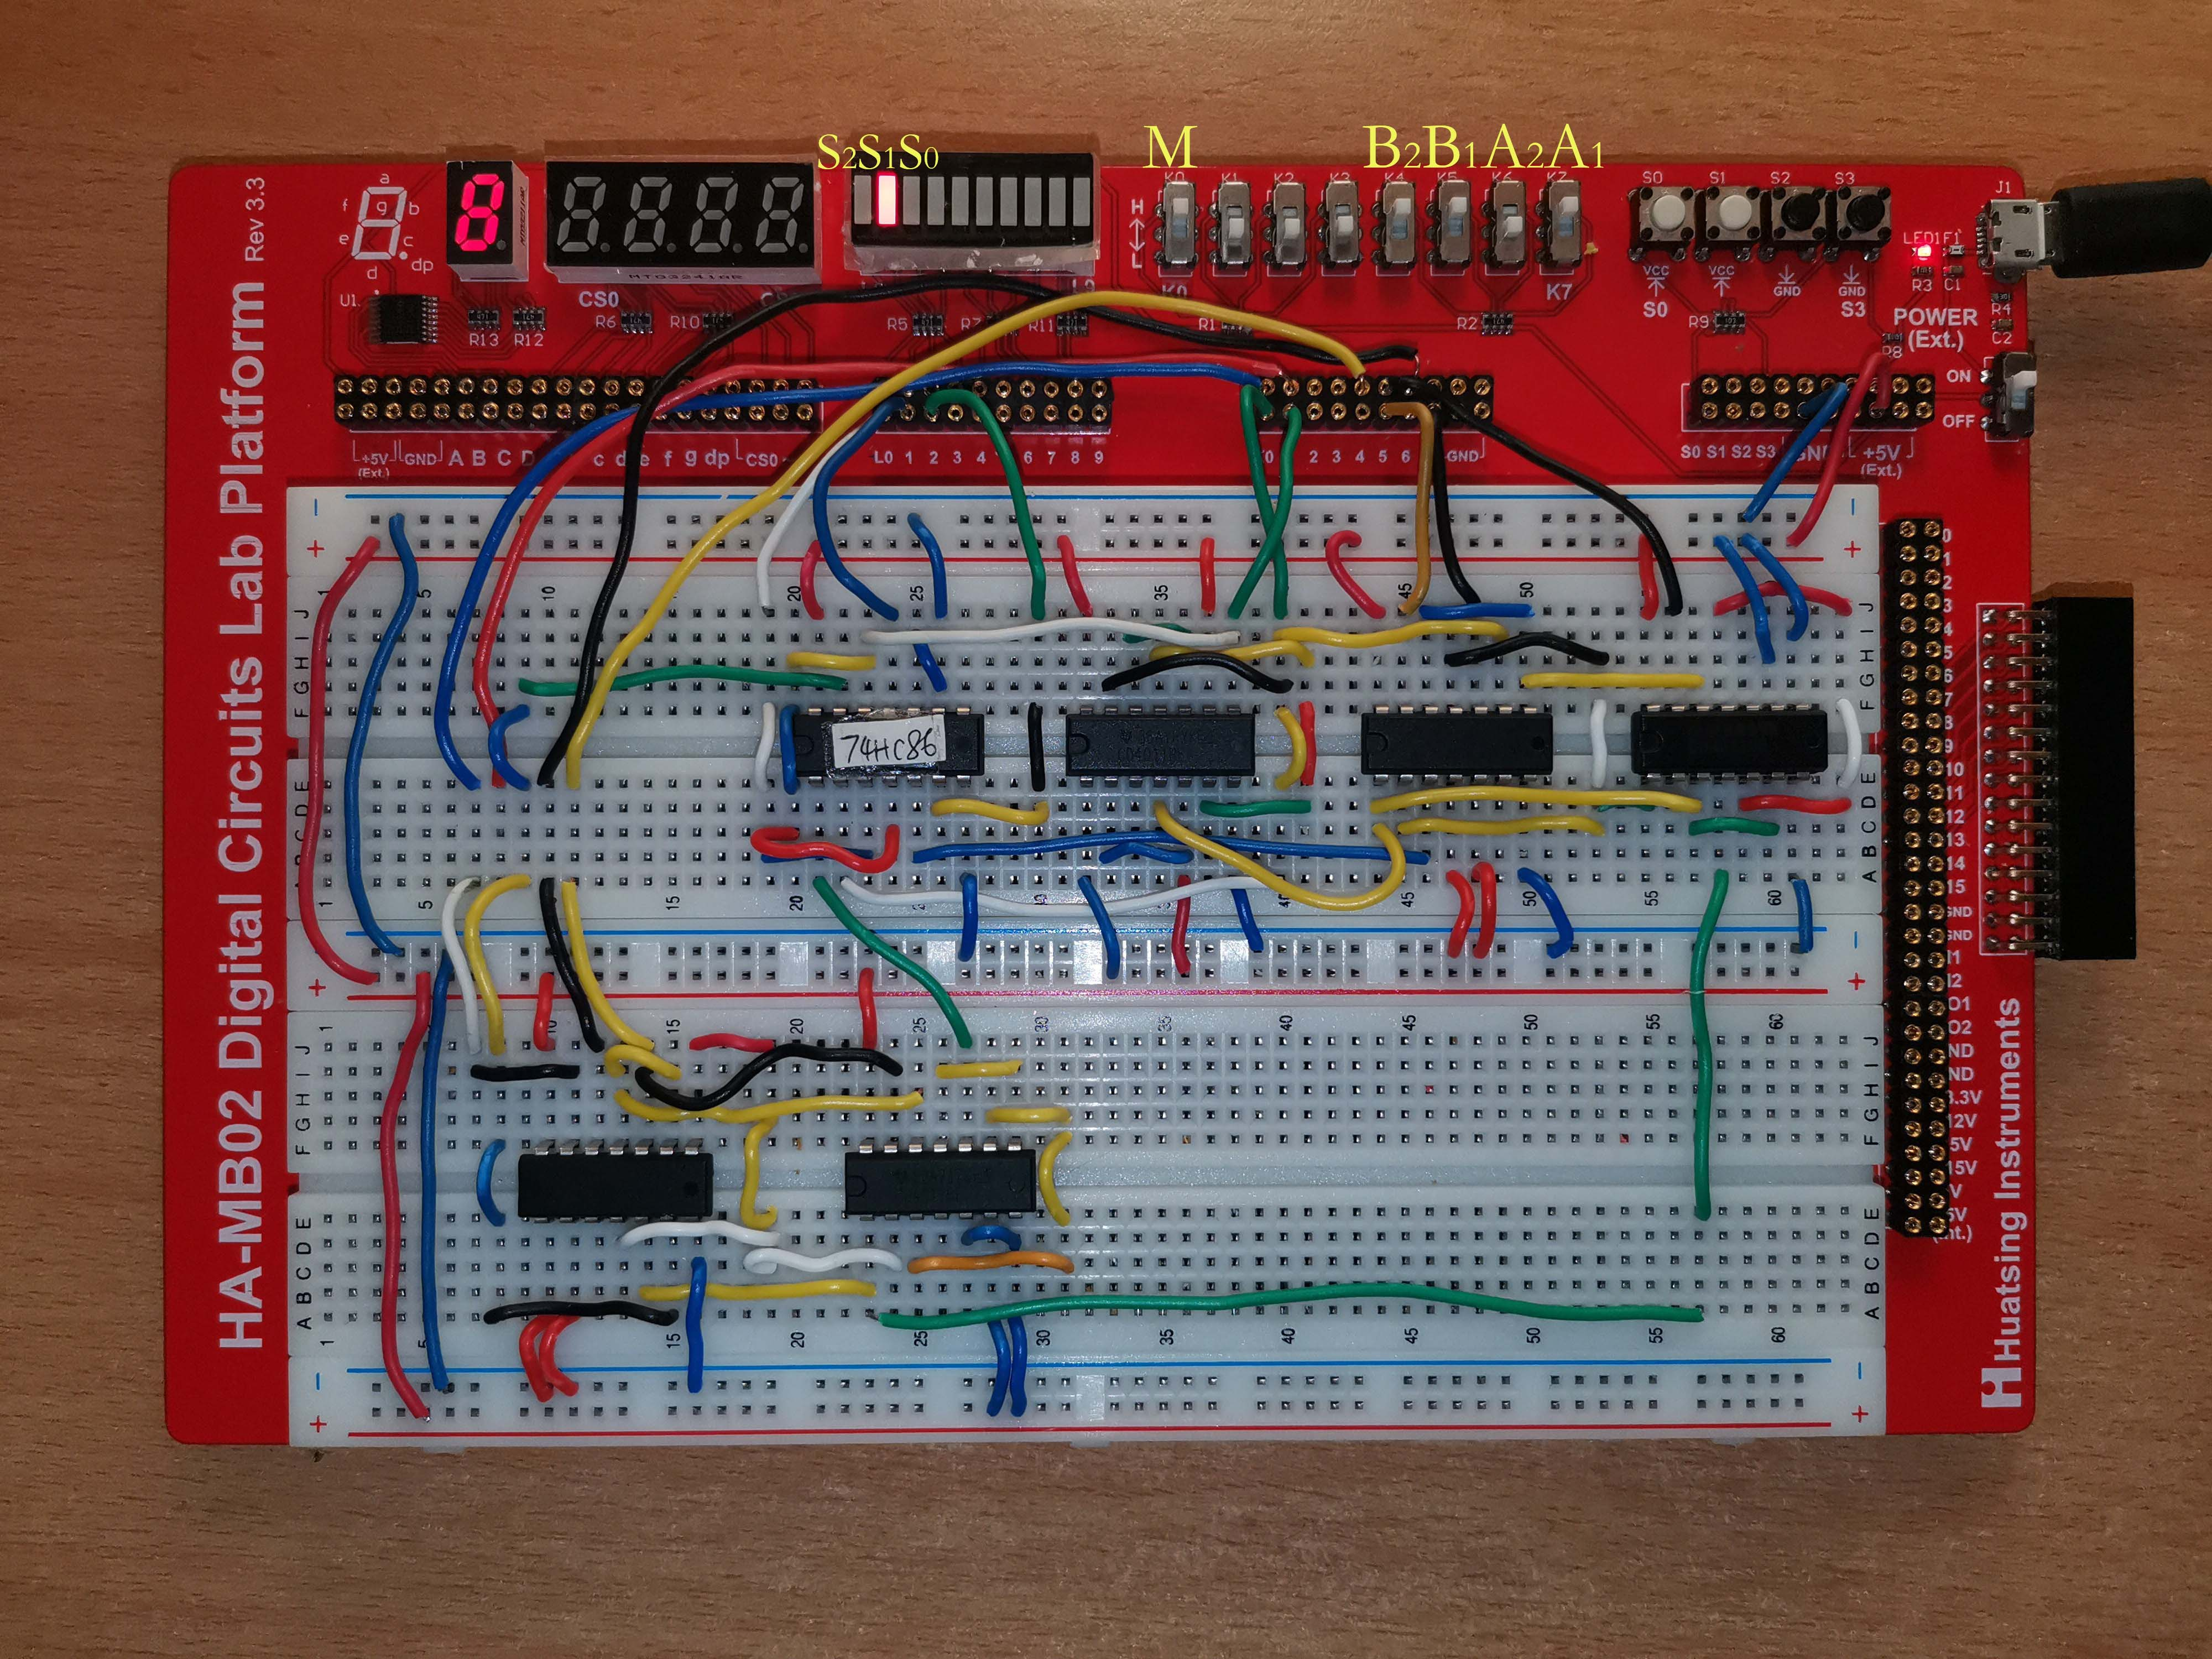
\includegraphics[scale=0.04]{3-1.jpg}}\hspace{0.3mm}    
    \subfigure[3-2]{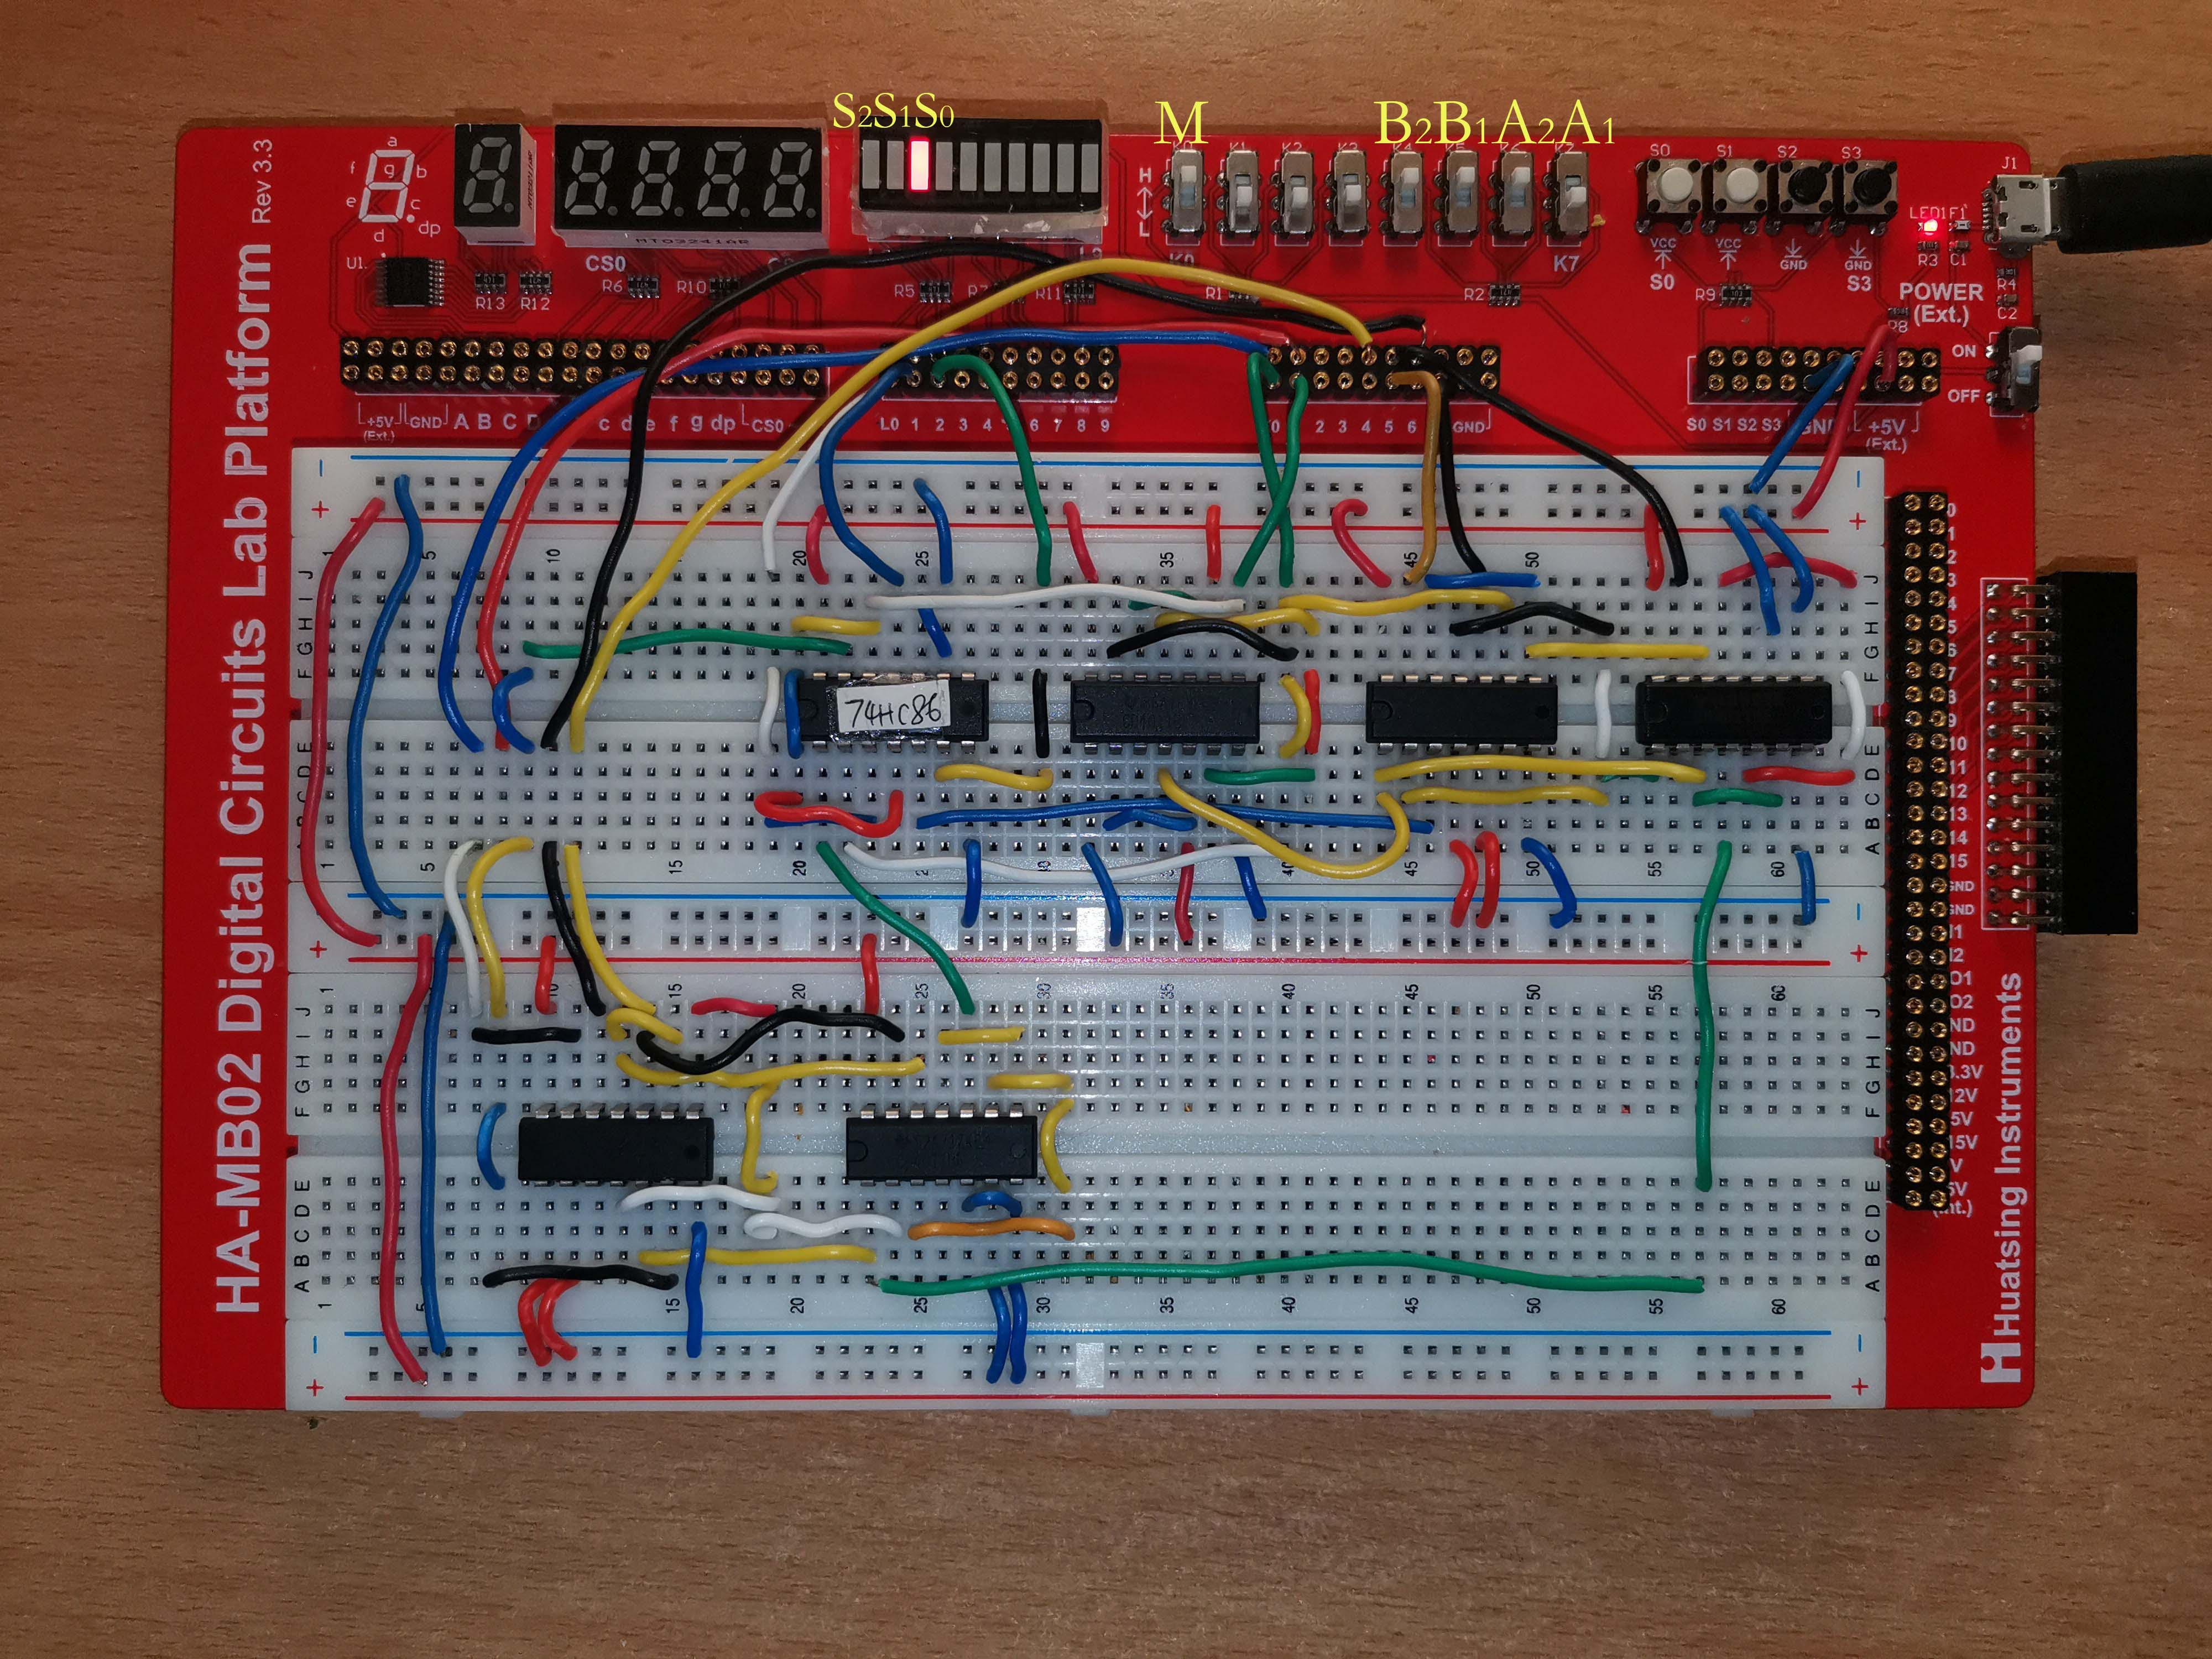
\includegraphics[scale=0.04]{3-2.jpg}}\hspace{0.3mm}
    \subfigure[2-3]{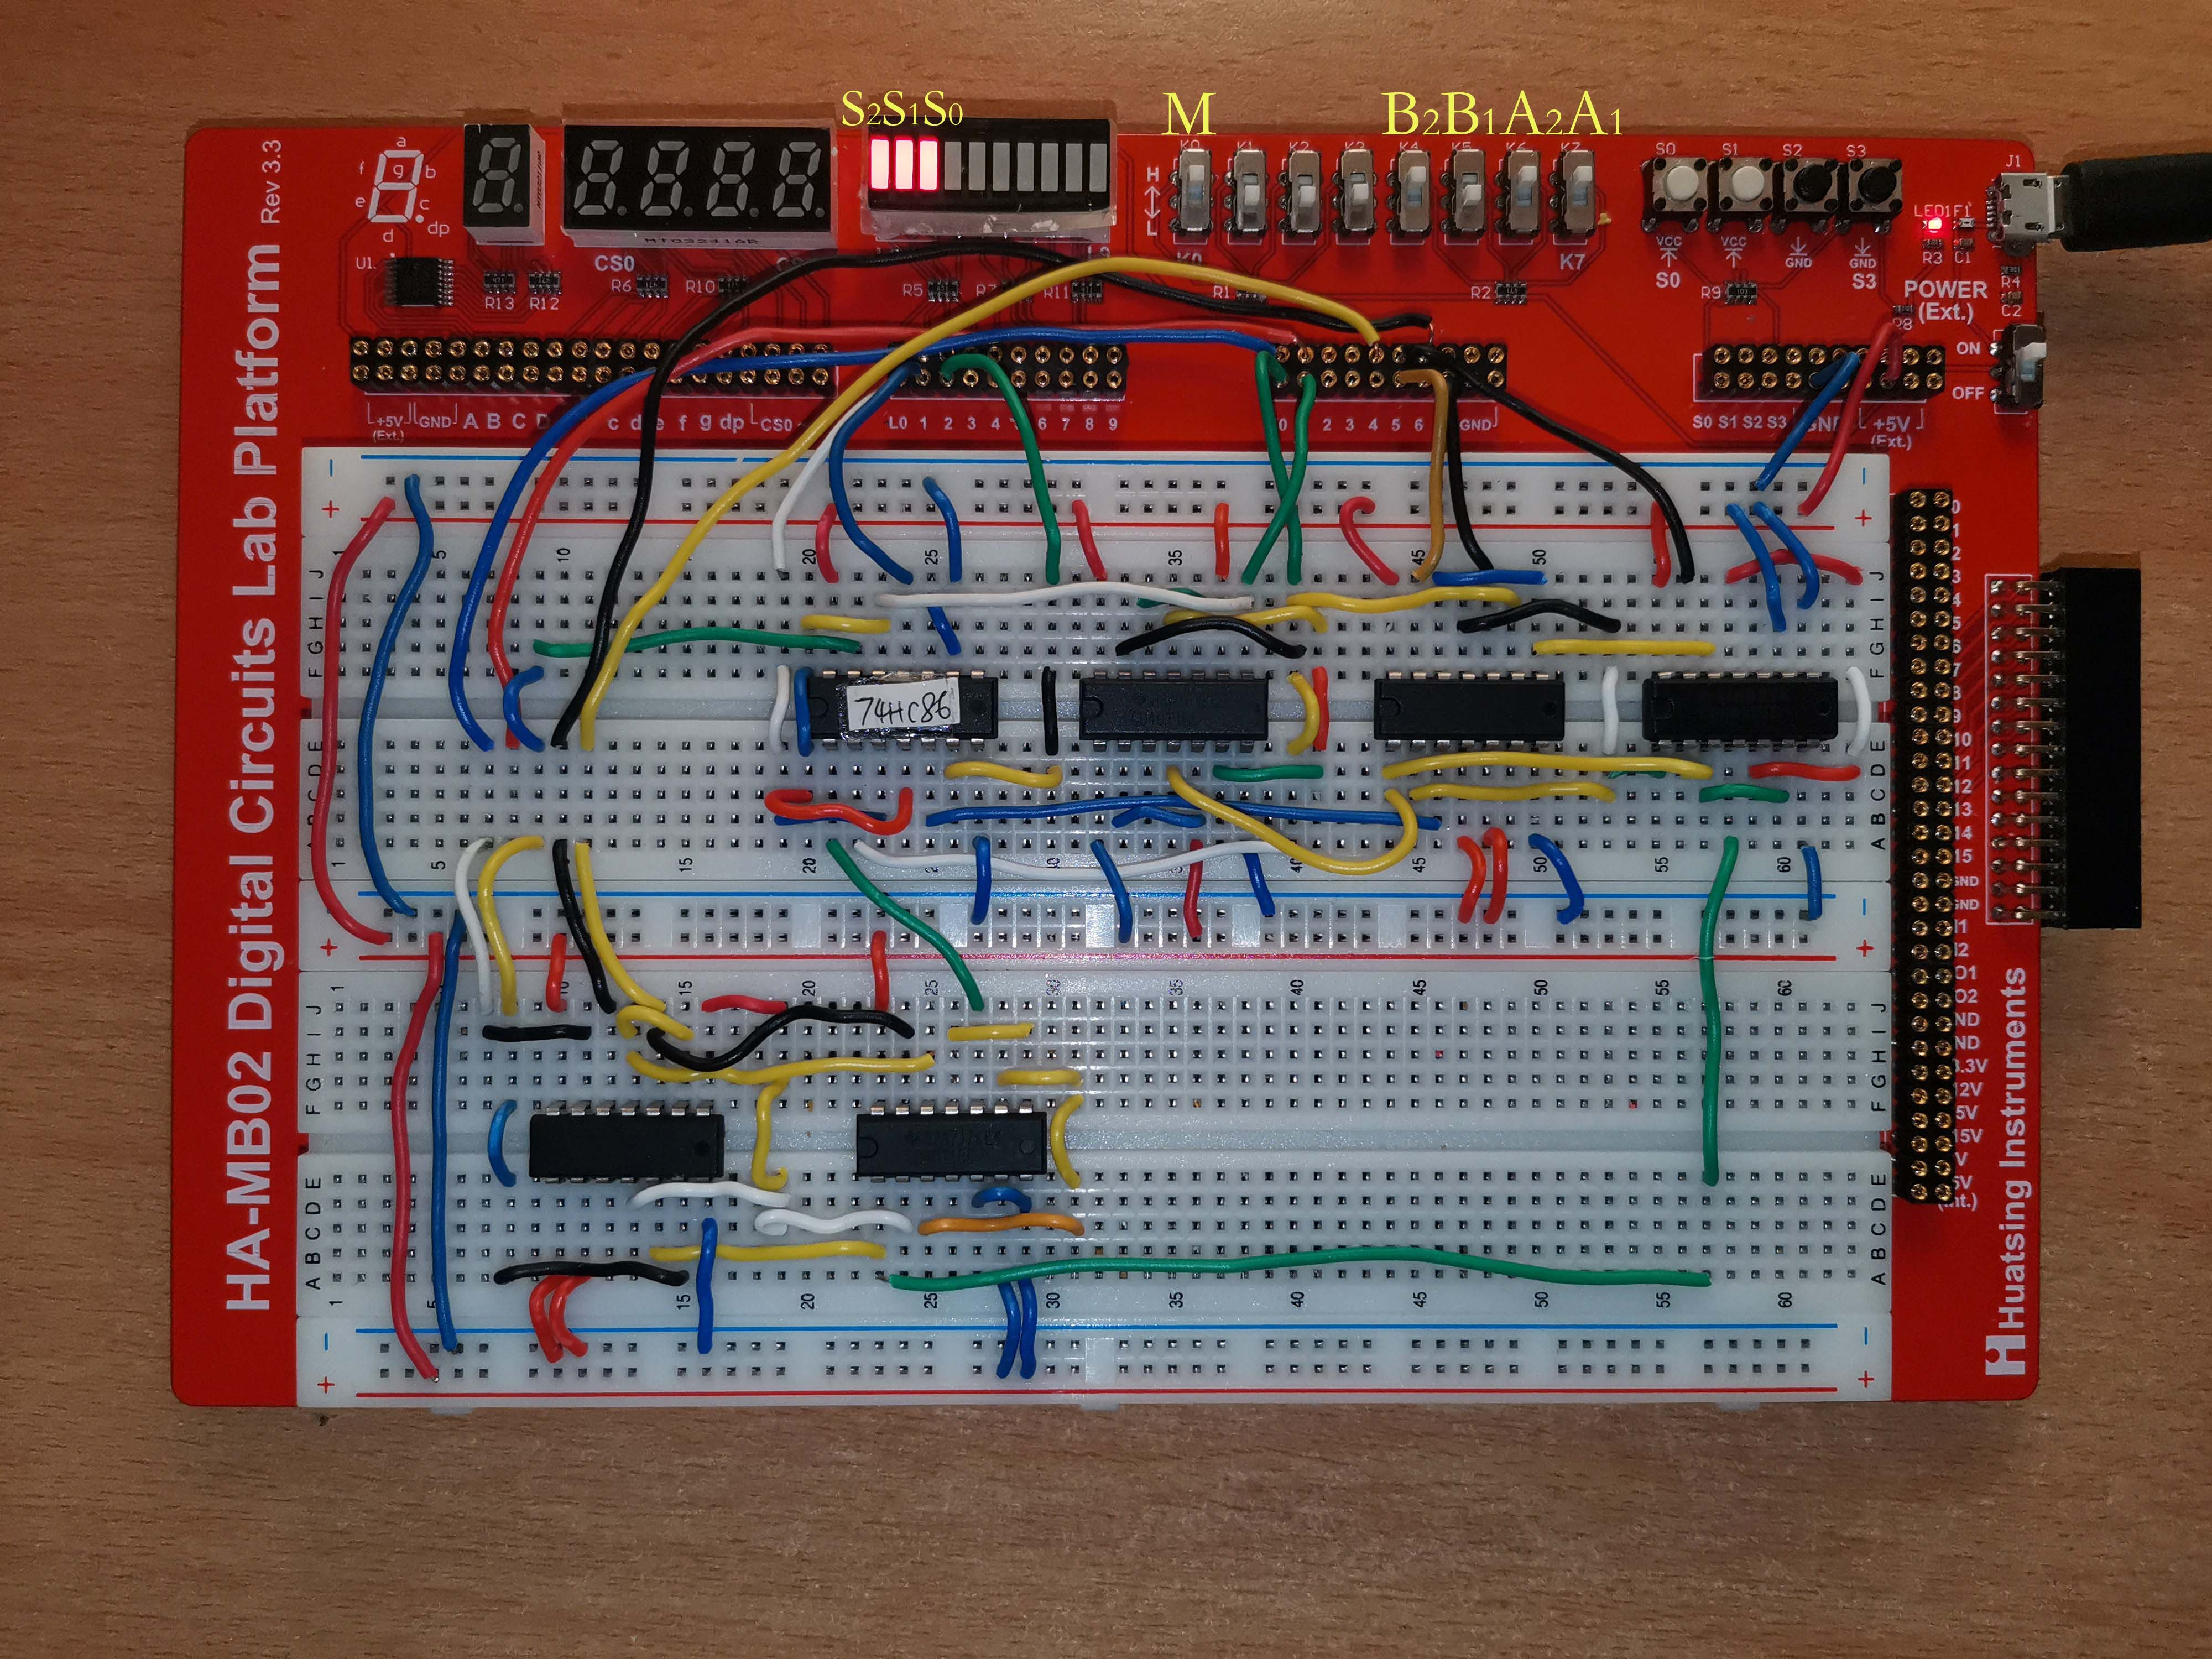
\includegraphics[scale=0.04]{2-3.jpg}}\hspace{0.3mm}
    \subfigure[1-3]{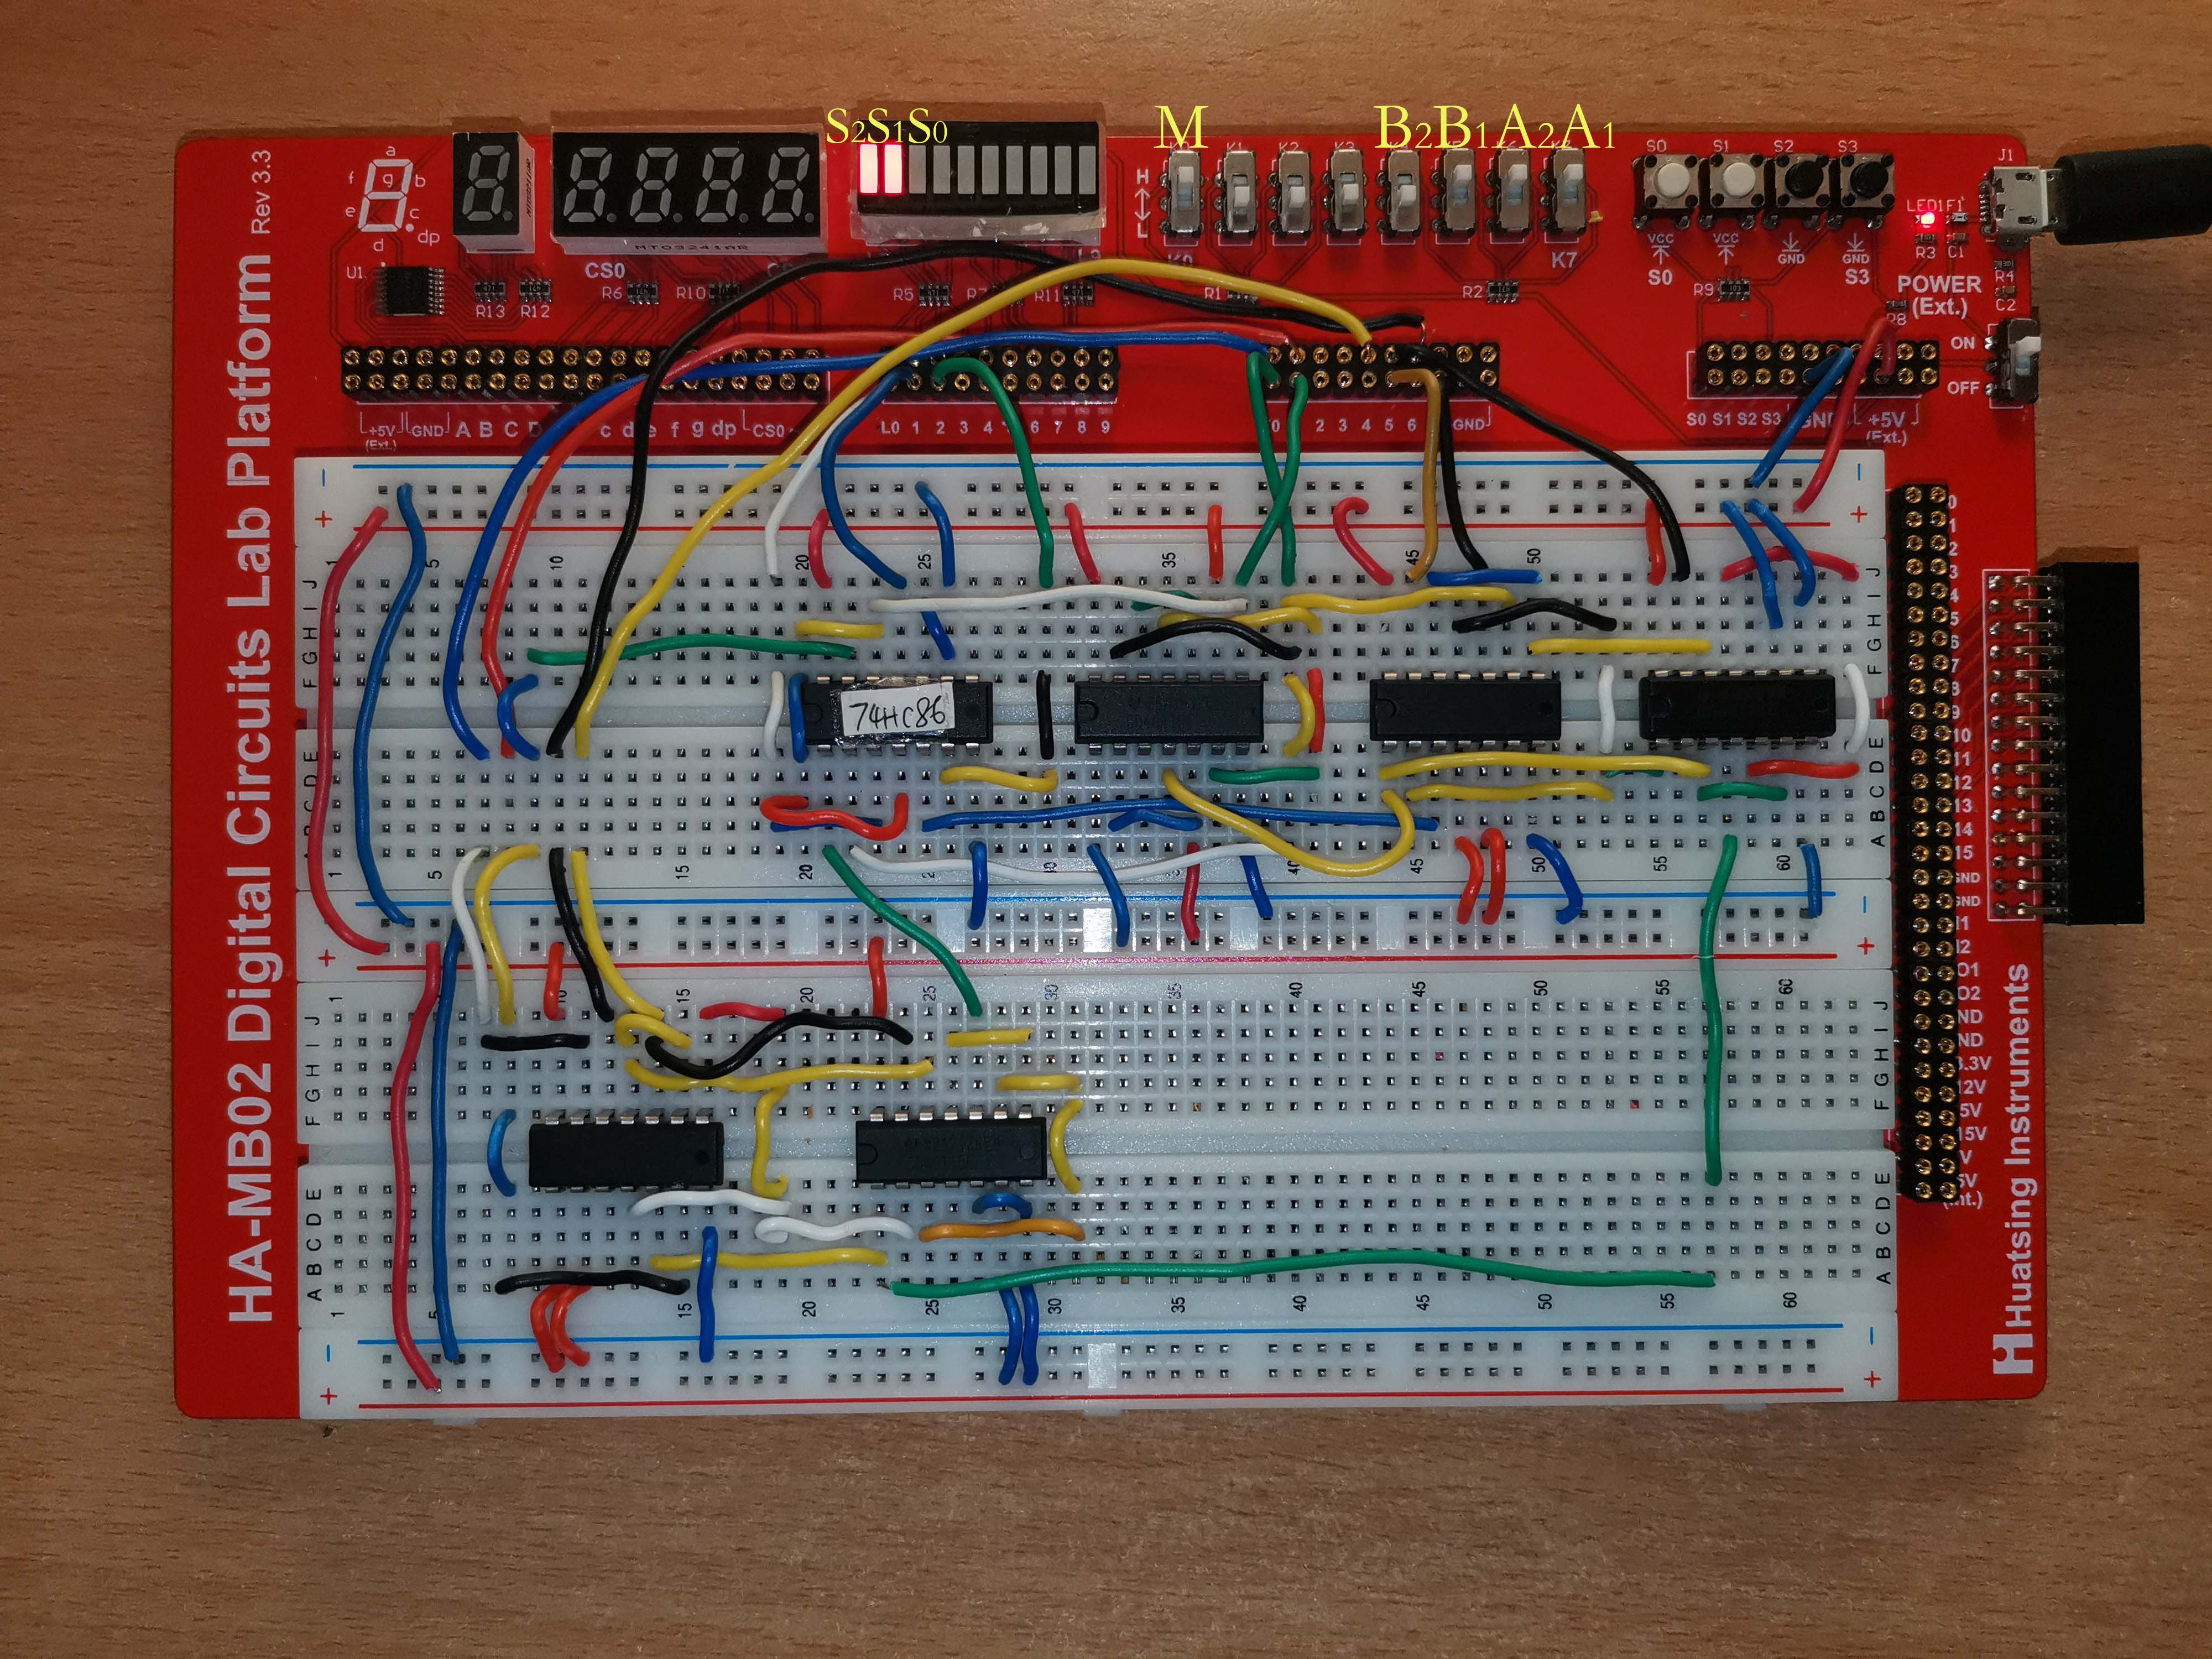
\includegraphics[scale=0.04]{1-3.jpg}}\hspace{0.3mm}
    \subfigure[0-3]{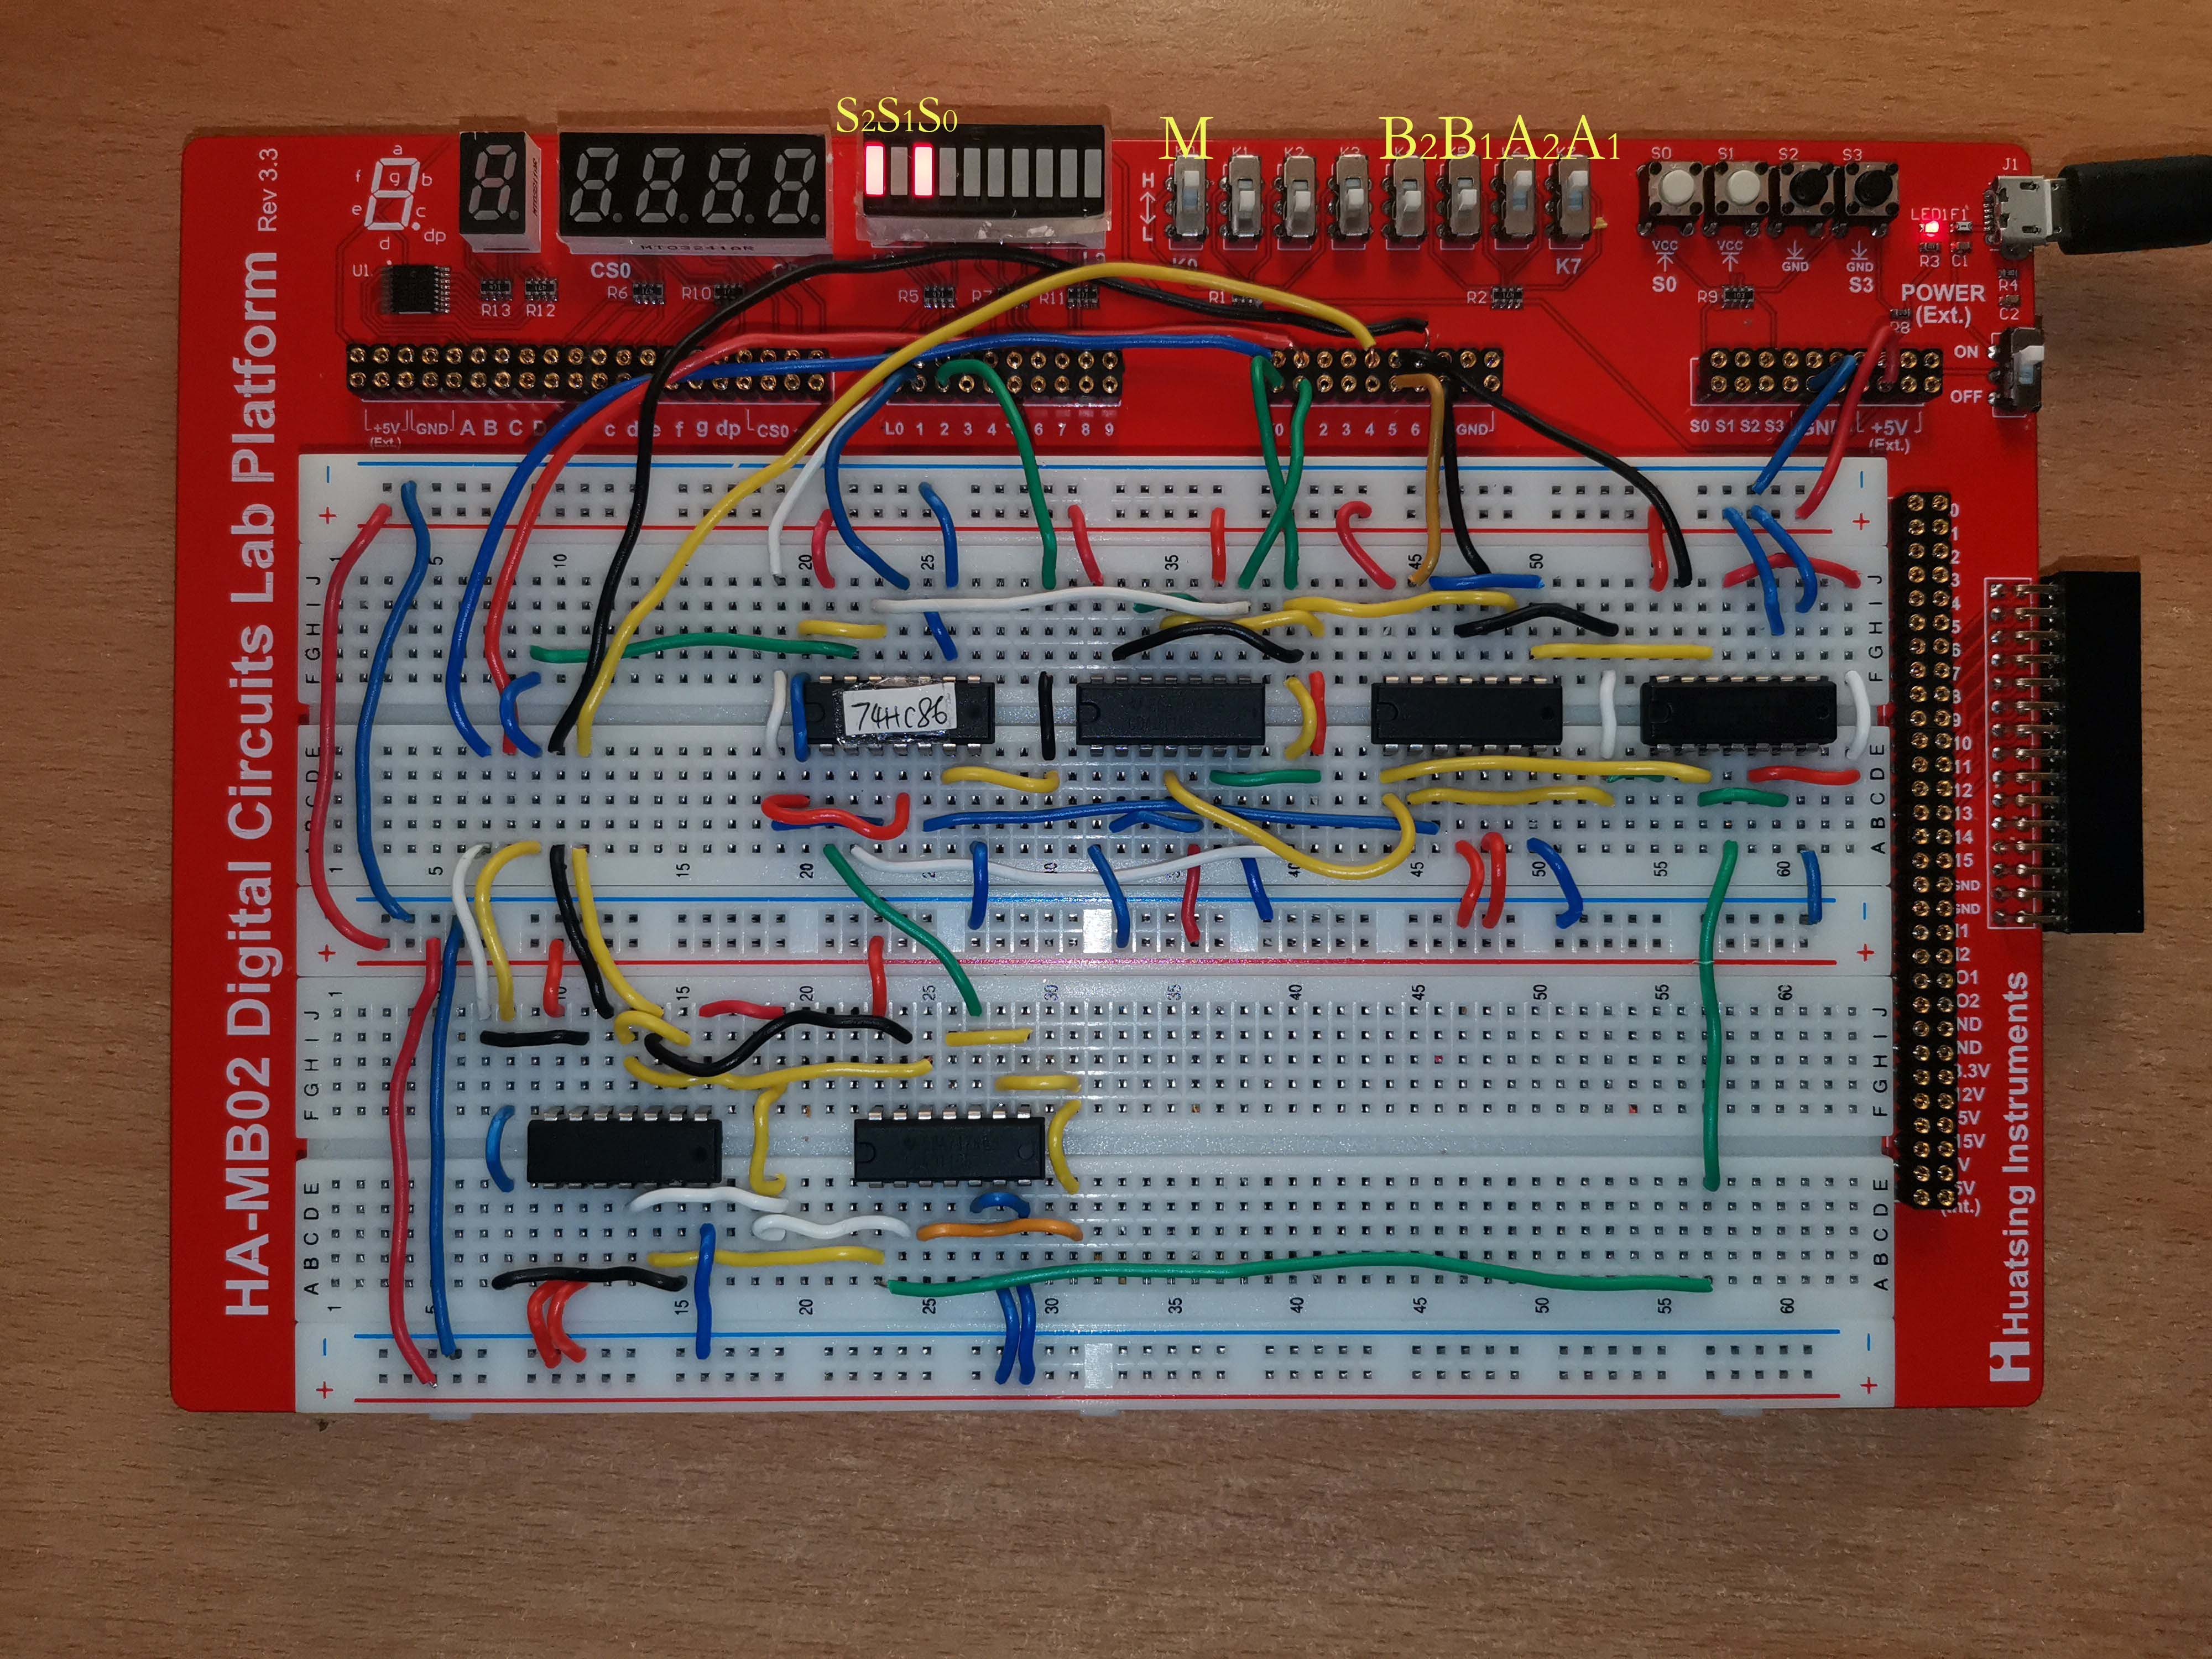
\includegraphics[scale=0.04]{0-3.jpg}}\hspace{0.3mm}
    \vspace{-1em}
    \caption{显示补码的减法器}
    \restoregeometry
    }
\end{figure}\par
\vspace{-1em}

\section{显示原码的二位减法器}
我们对上述“用补码显示的二位减法器”进行一定的修改即可得到原码显示的减法器.\par
我们列出原码$(Y_2Y_1Y_0)_2$和其补码值(已经求出)$(S_2S_1S_0)_2$的真值表:
\begin{table}[H]
    \begin{center}
    \begin{tabular}{p{4em}<{\centering}|p{4em}<{\centering}|p{4em}<{\centering}|p{4em}<{\centering}|p{4em}<{\centering}|p{4em}<{\centering}}
        \hline\hline
        $S_2$&$S_1$&$S_0$&$Y_2$&$Y_1$&$Y_0$\\
        \hline
        0&1&1&0&1&1\\
        \hline
        0&1&0&0&1&0\\
        \hline
        0&0&1&0&0&1\\
        \hline
        0&0&0&0&0&0\\
        \hline
        1&1&1&1&0&1\\
        \hline
        1&1&0&1&1&0\\
        \hline
        1&0&1&1&1&1\\
        \hline
    \end{tabular}
\end{center}\end{table}
约束条件是$S_2S_1'S_0'=0$(减法得出的运算结果,其补码不可能是100).
我们可以得到
\[Y_2=S_2S_1S_0+S_2S_1S_0'+S_2S_1'S_0\]
\[Y_0=S_2'S_1S_0+S_2'S_1'S_0+S_2S_1S_0+S_2S_1'S_0\]
\[Y_1=S_2'S_1S_0+S_2'S_1S_0'+S_2S_1S_0'+S_2S_1'S_0\]
画出卡诺图如下:
\begin{figure}[H]\centering
    {
        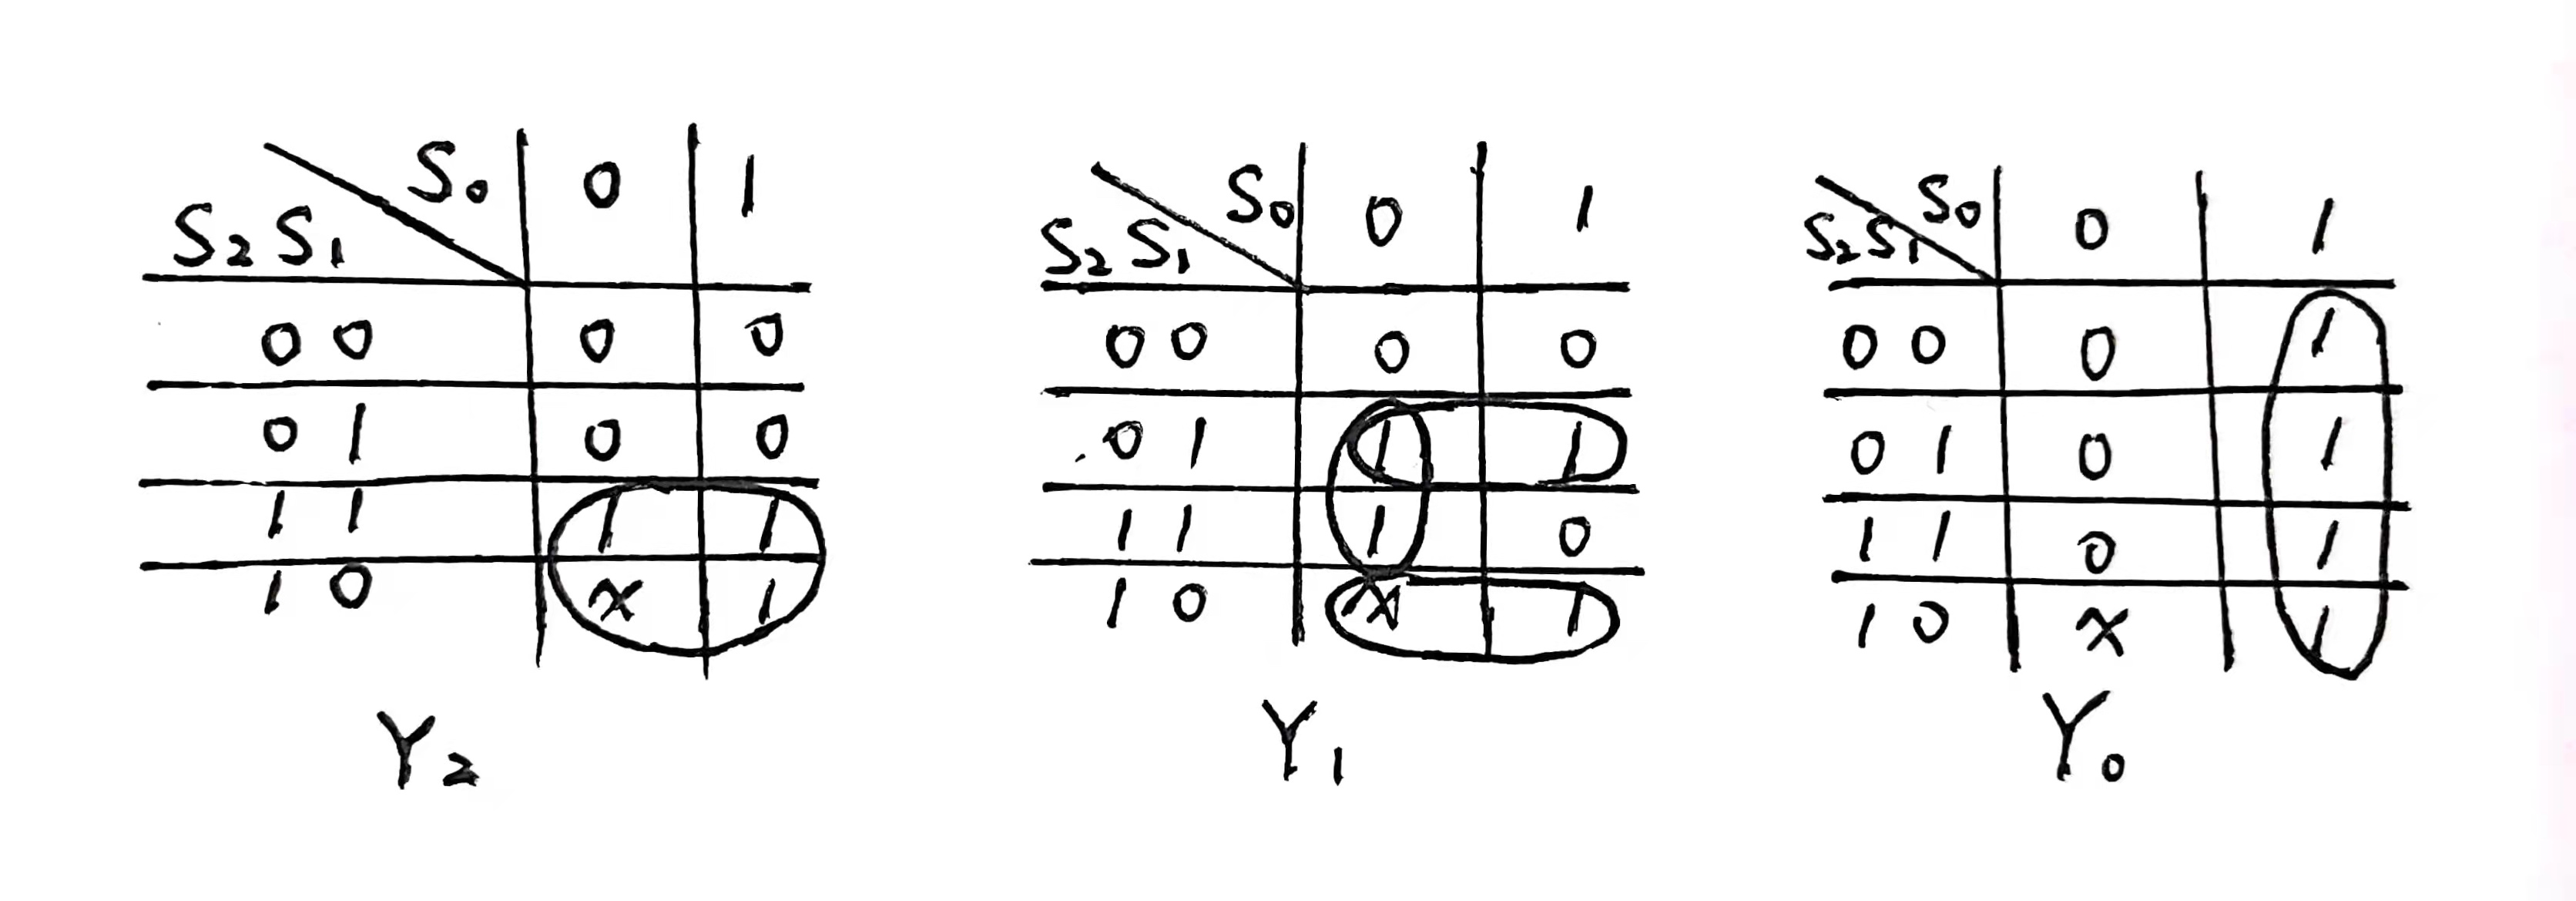
\includegraphics[scale=0.1]{6.jpg}
        \caption{$Y_2Y_1Y_0$卡诺图}
    }
\end{figure}\par
因此有
\[Y_2=S_2\]
\[Y_0=S_0\]
$$
\begin{aligned}
    Y_1&=S_1S_0'+(S_2'S_1+S_2S_1')S_0\\
    &=S_0'S_1+S_0(S_1\oplus S_2)\\
    &=((S_0'S_1)'\cdot(S_0(S_1\oplus S_2))')'
\end{aligned}
$$

因此可以将减法(补码)运算器电路图改装为下图(M取1):
\begin{figure}[H]\centering
    {
        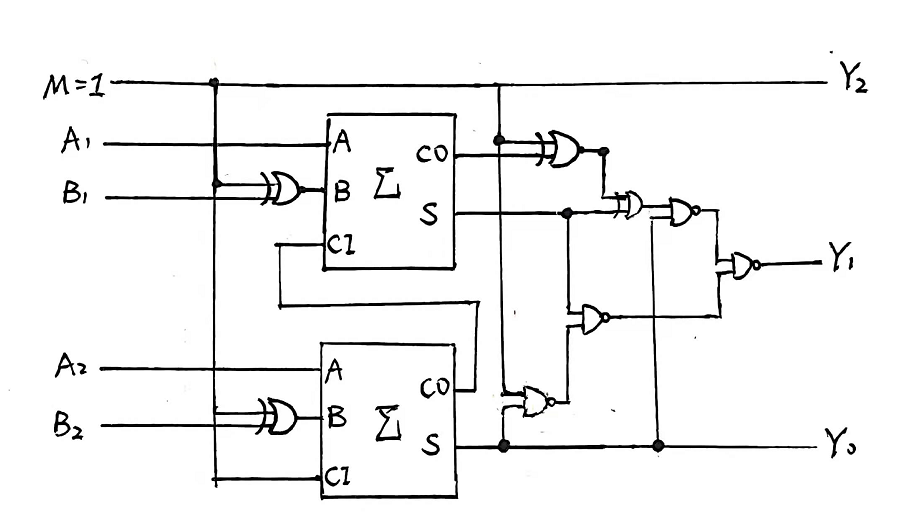
\includegraphics[scale=0.5]{5.PNG}
        \caption{减法(补码)运算器电路图}
    }
\end{figure}\par

\subsection{电路实物图}
\begin{figure}[H]\centering
    {
        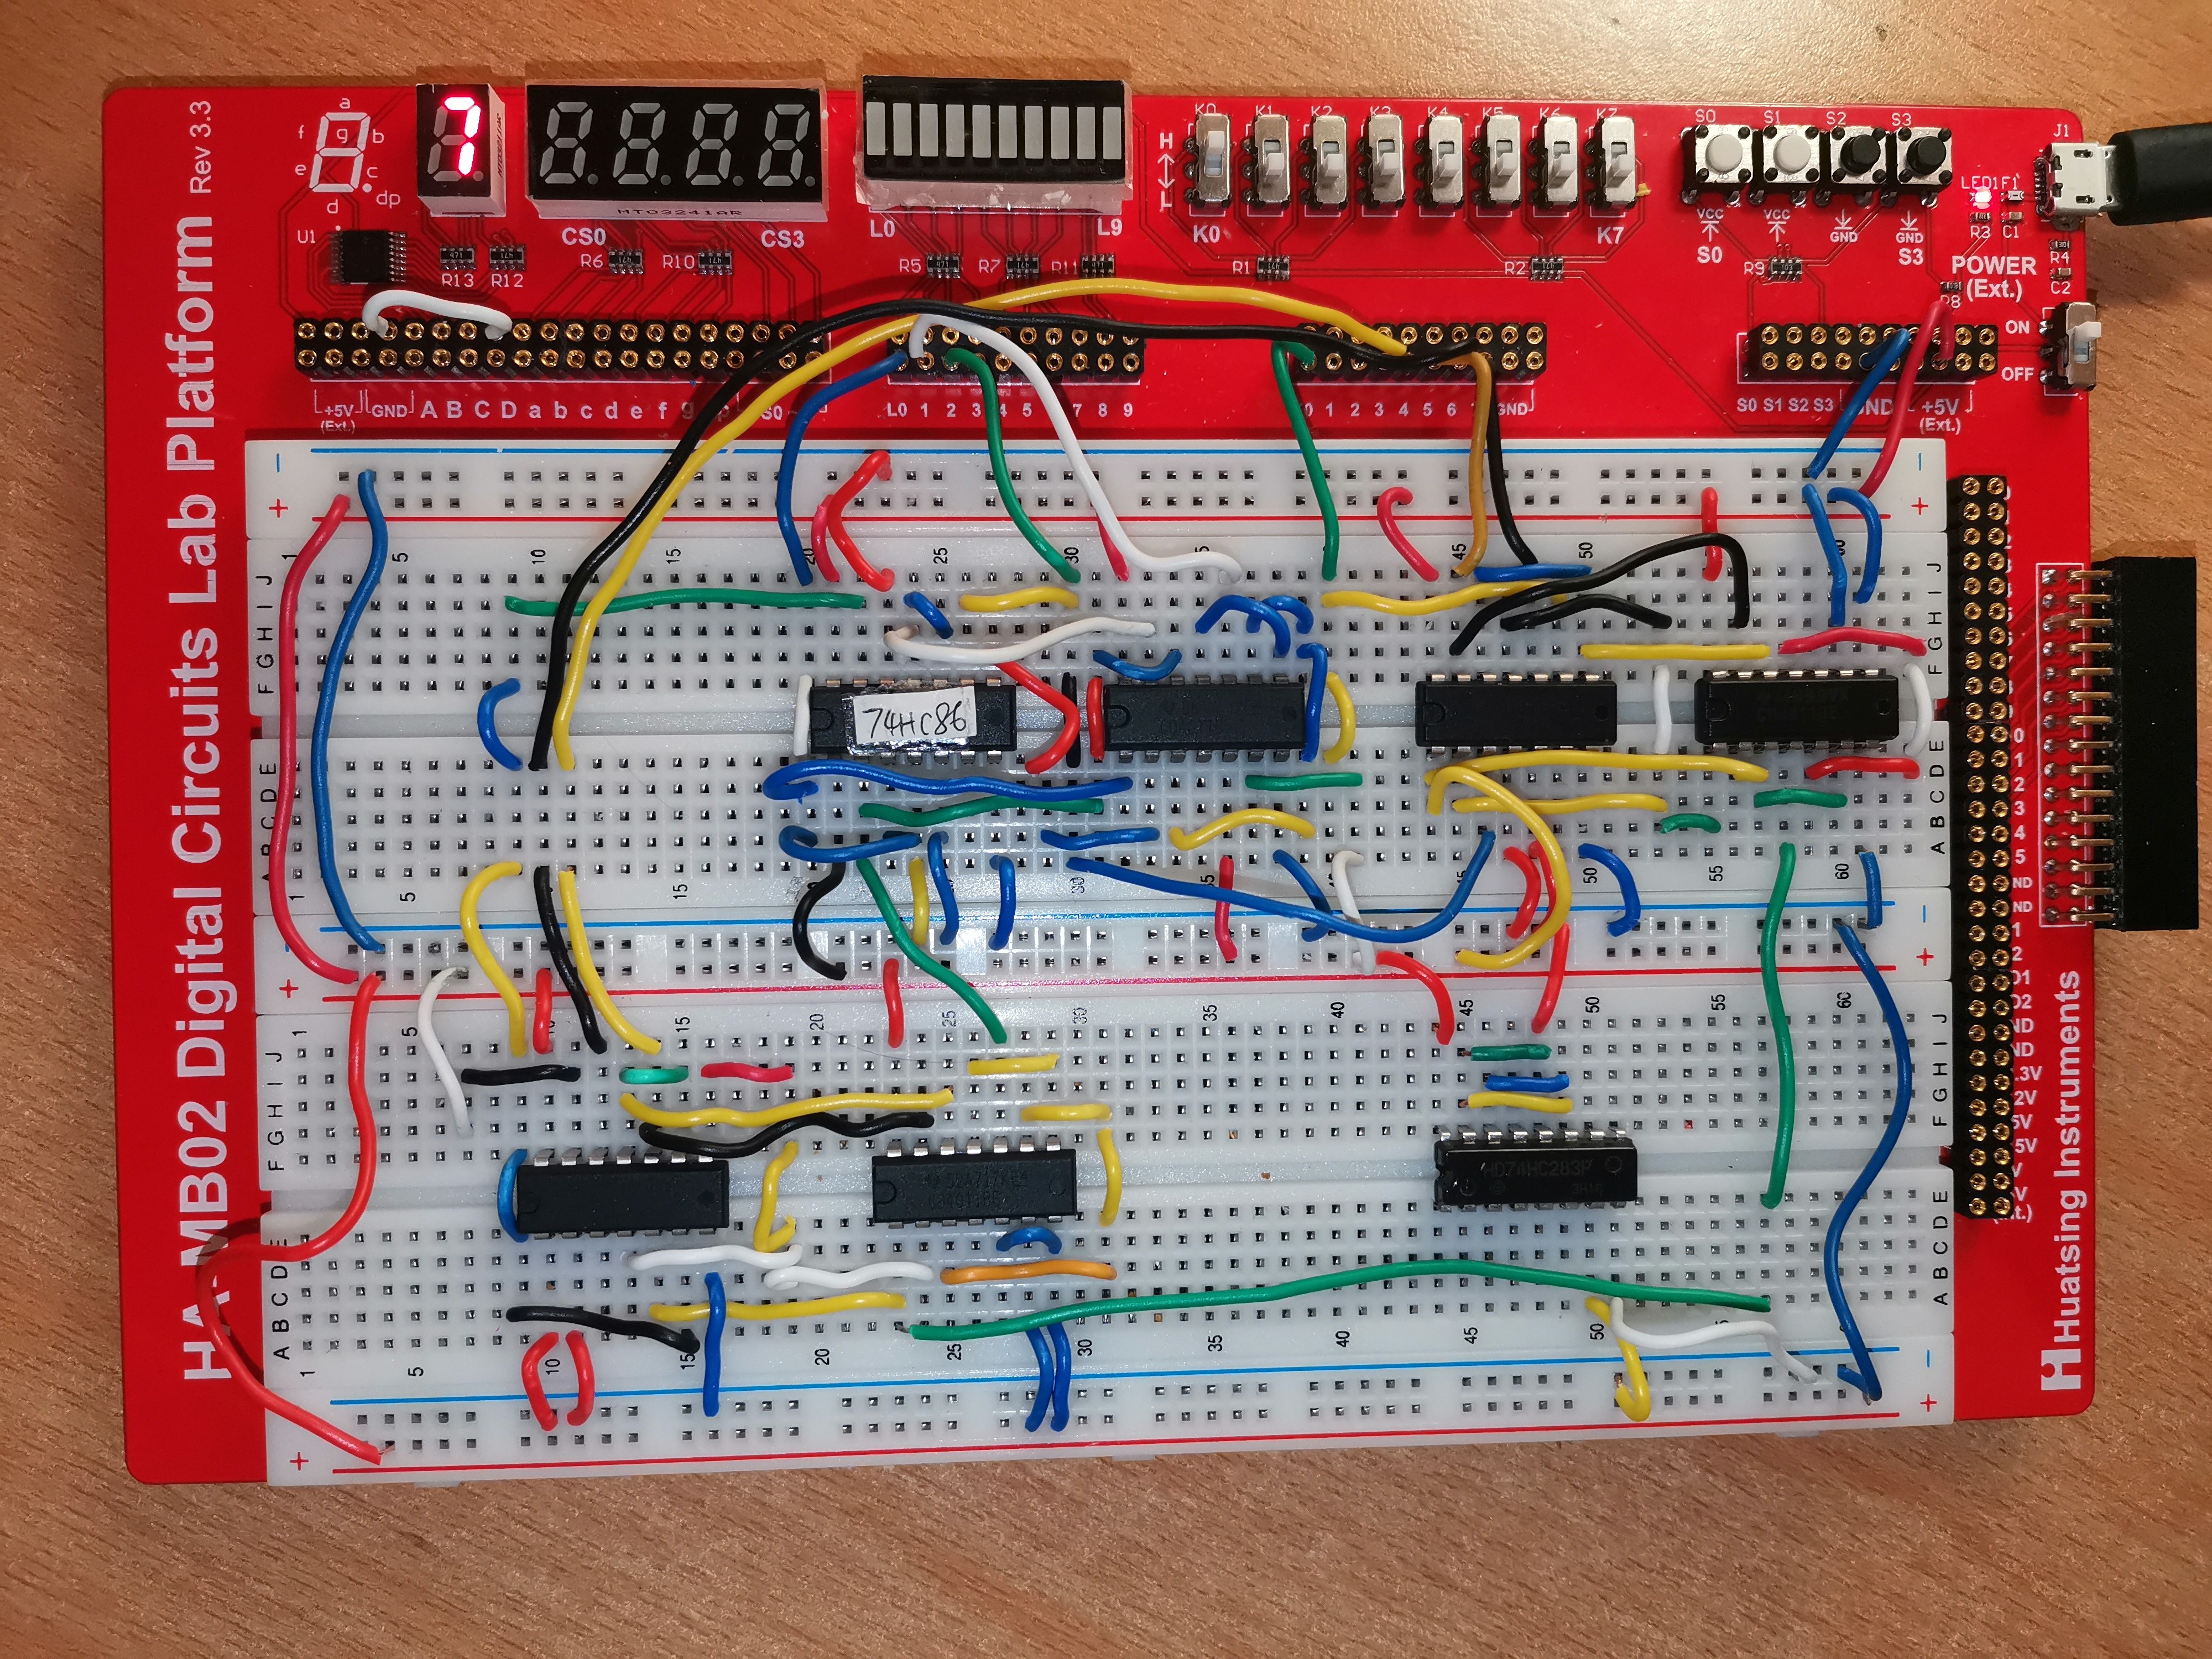
\includegraphics[scale=0.08]{20.jpg}
        \caption{用原码显示的二位减法器}
    }
\end{figure}\par
\vspace{-2em}
\subsection{功能展示}


\begin{figure}[H]\centering
    {
    \setcounter{subfigure}{0}
    \newgeometry{a4paper,left=3cm,right=0cm}
    \vspace{-1em}
    \subfigcapskip=-10pt
    \subfigure[0-1]{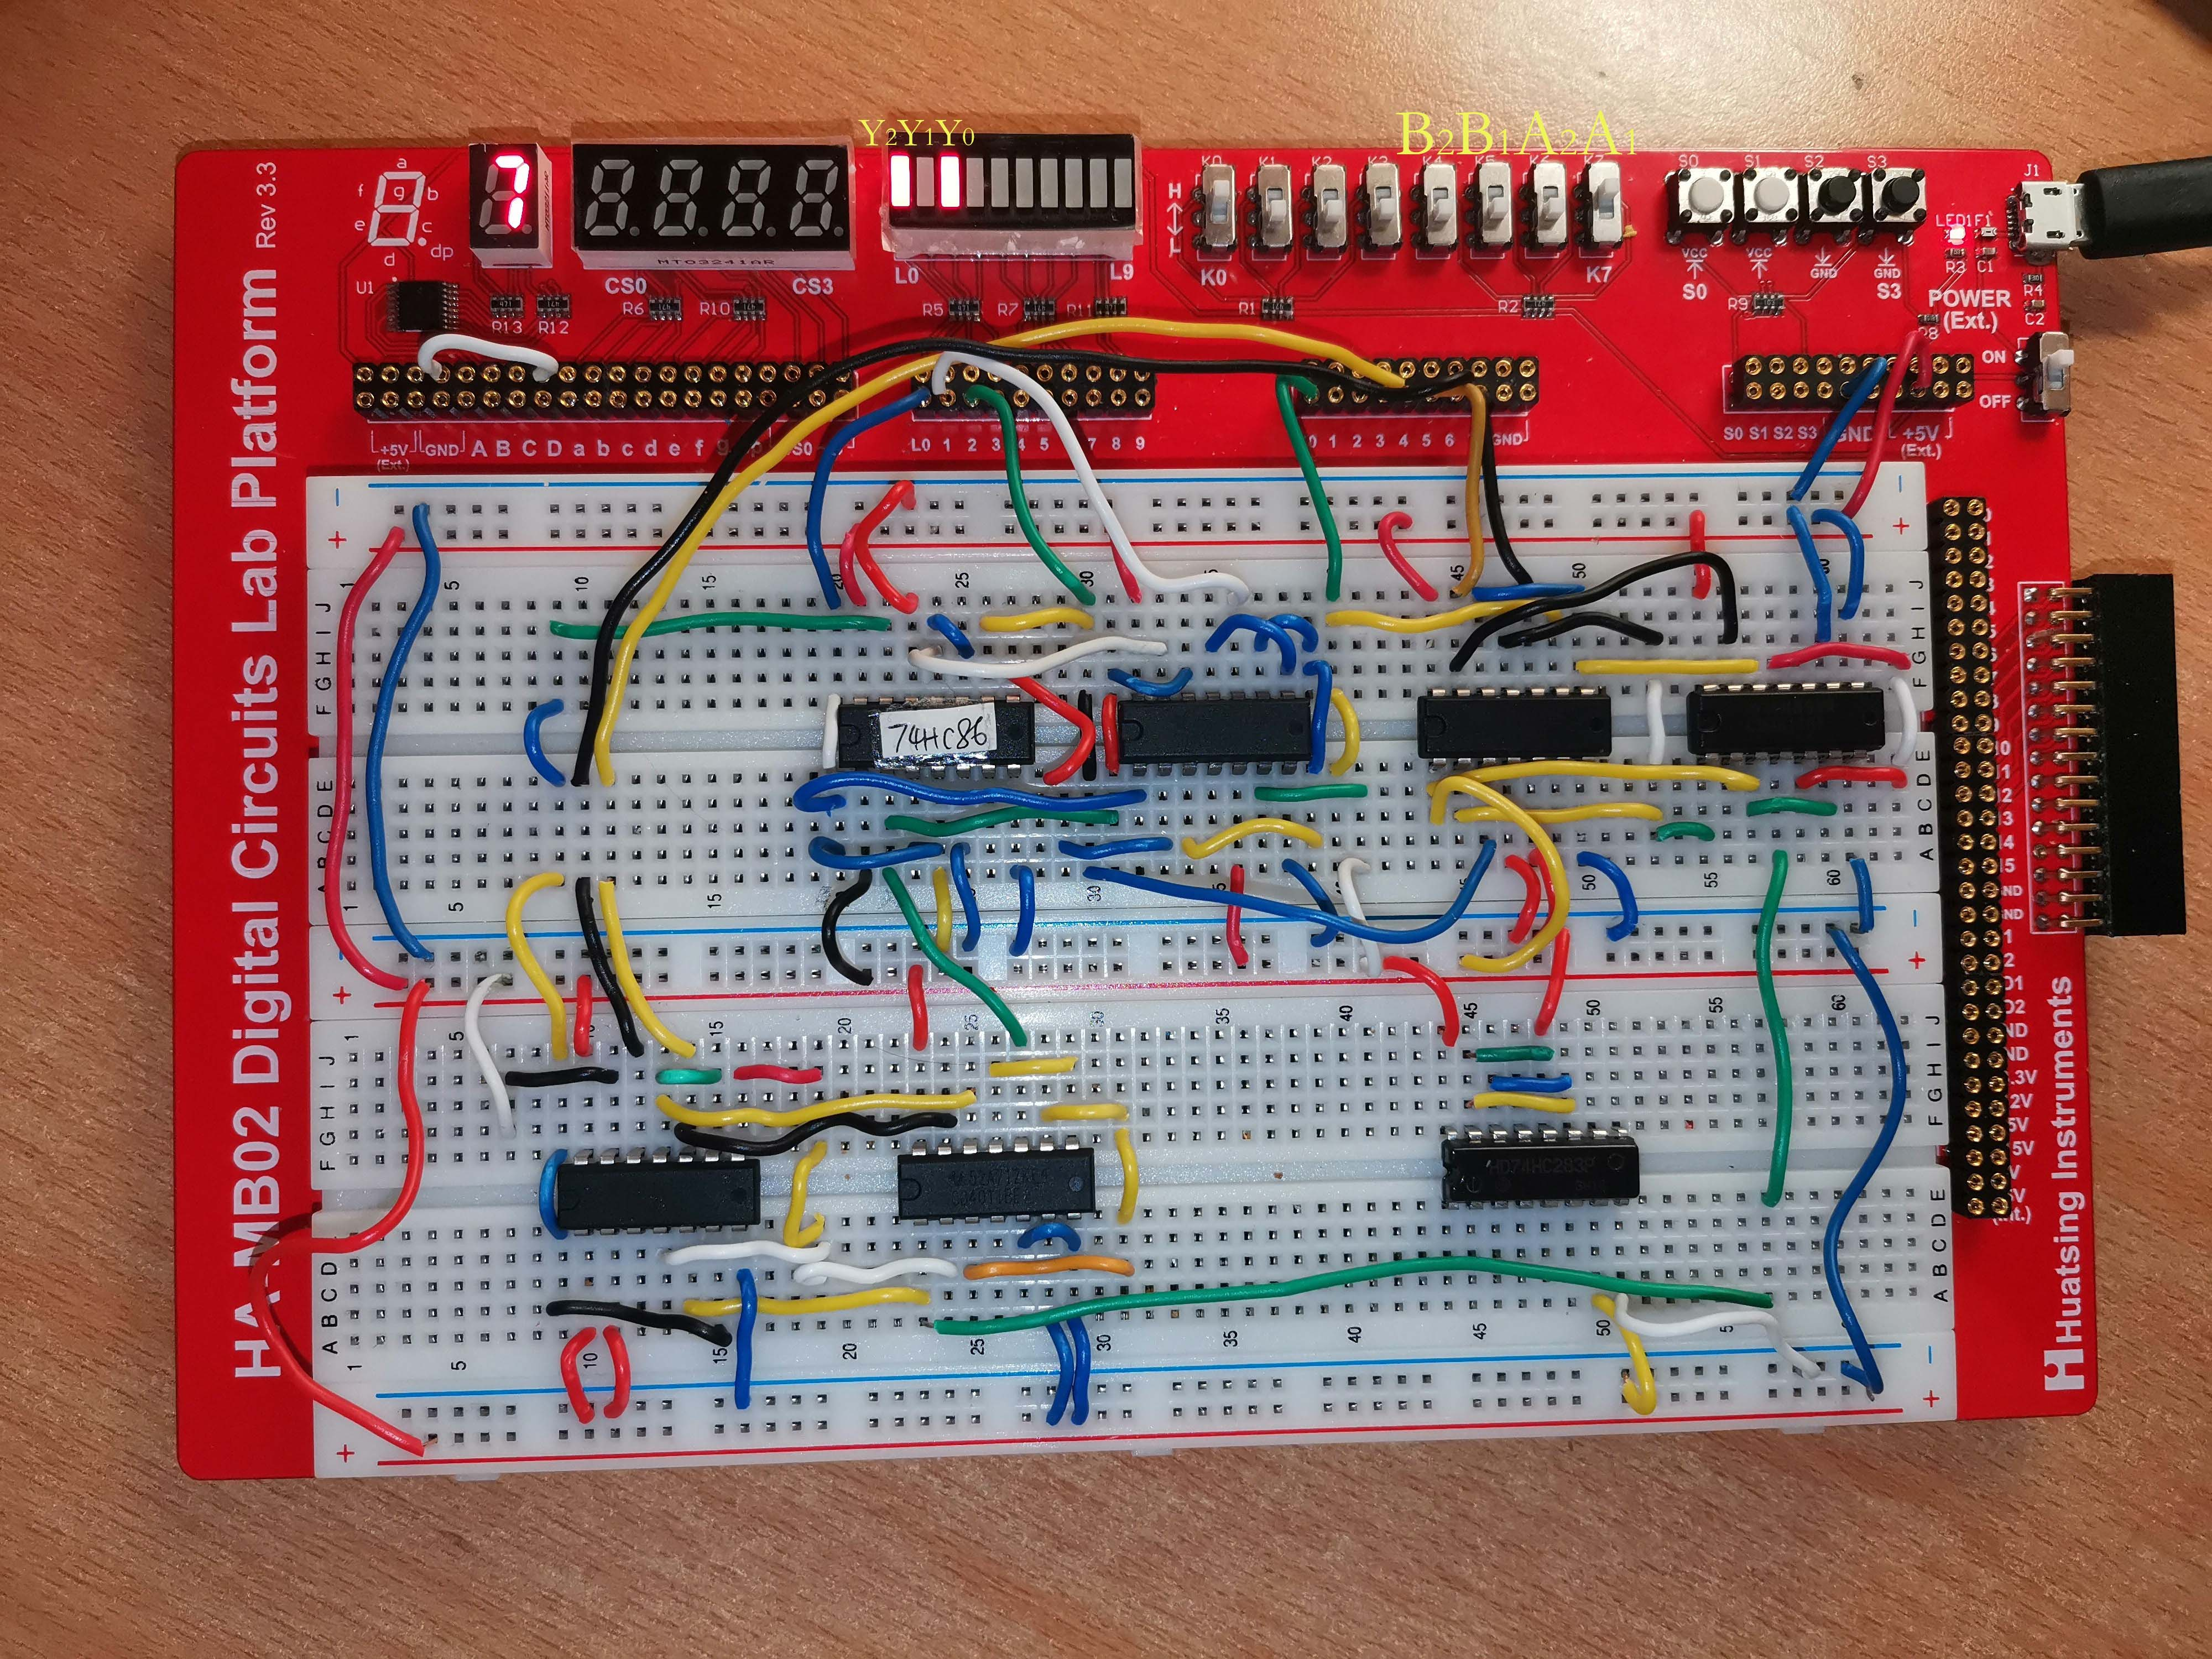
\includegraphics[scale=0.04]{0-1'.jpg}}\hspace{0.3mm}
    \subfigure[0-2]{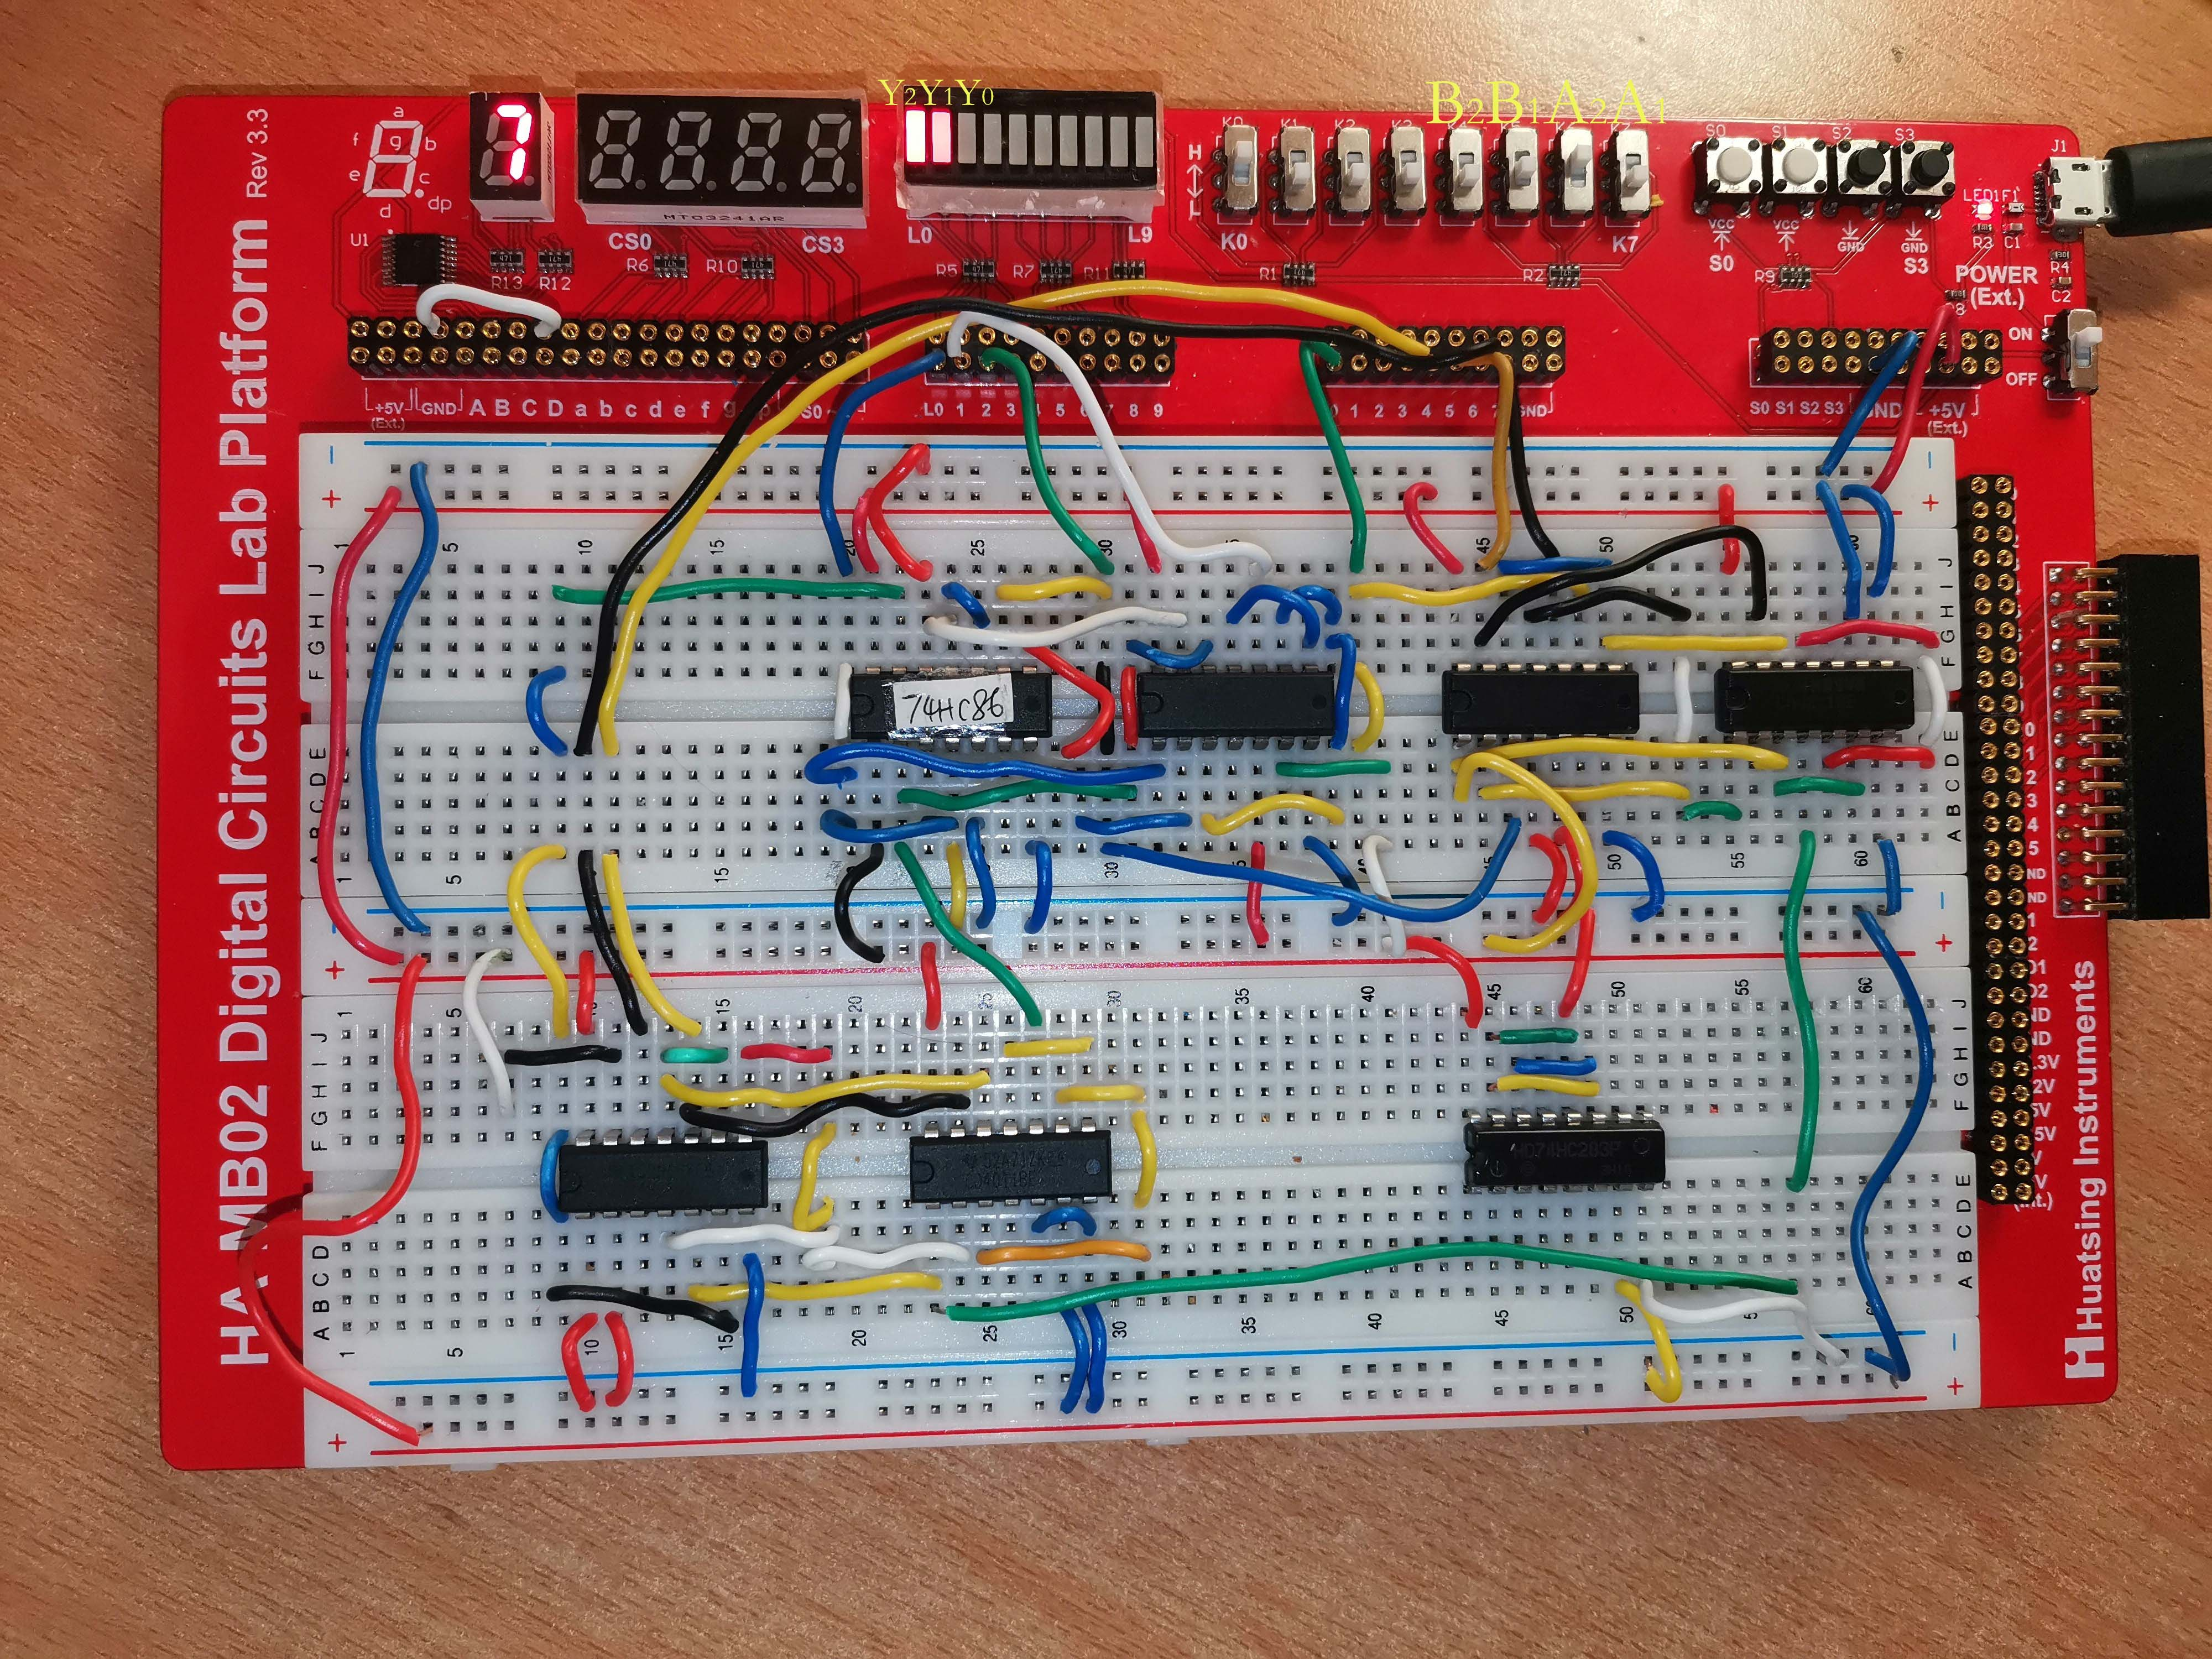
\includegraphics[scale=0.04]{0-2'.jpg}}\hspace{0.3mm}    
    \subfigure[0-3]{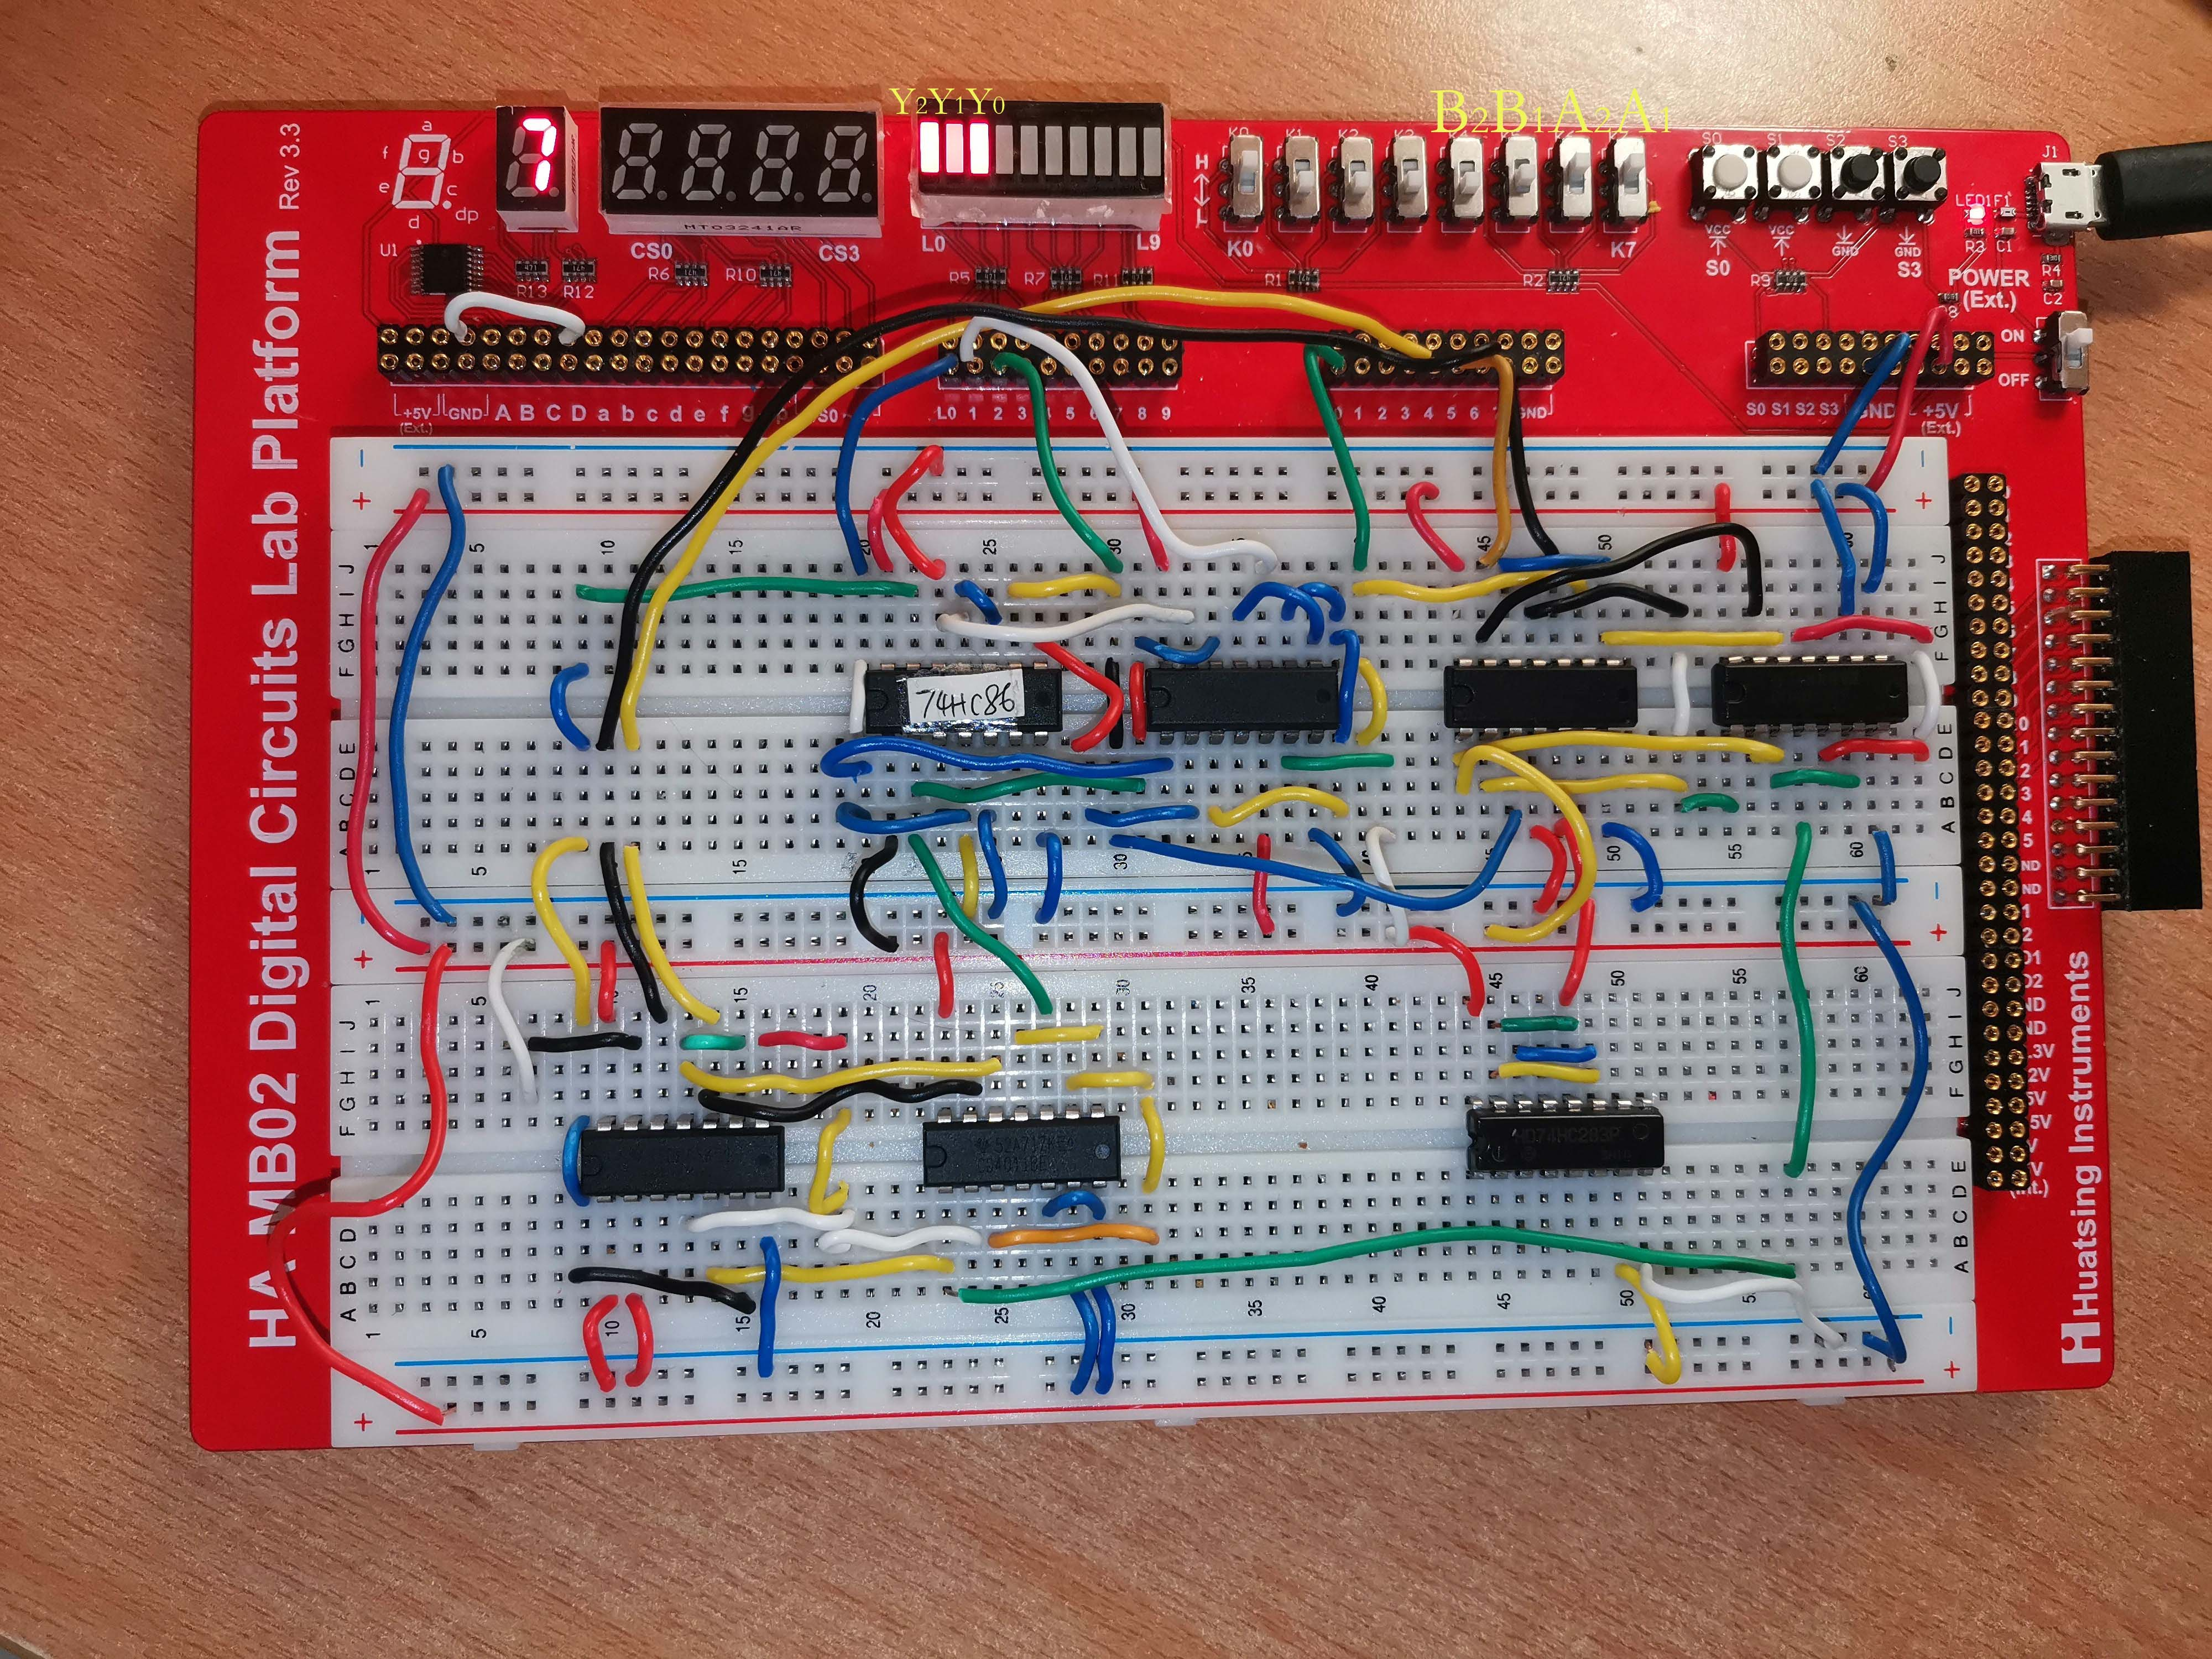
\includegraphics[scale=0.04]{0-3'.jpg}}\hspace{0.3mm}
    \subfigure[1-3]{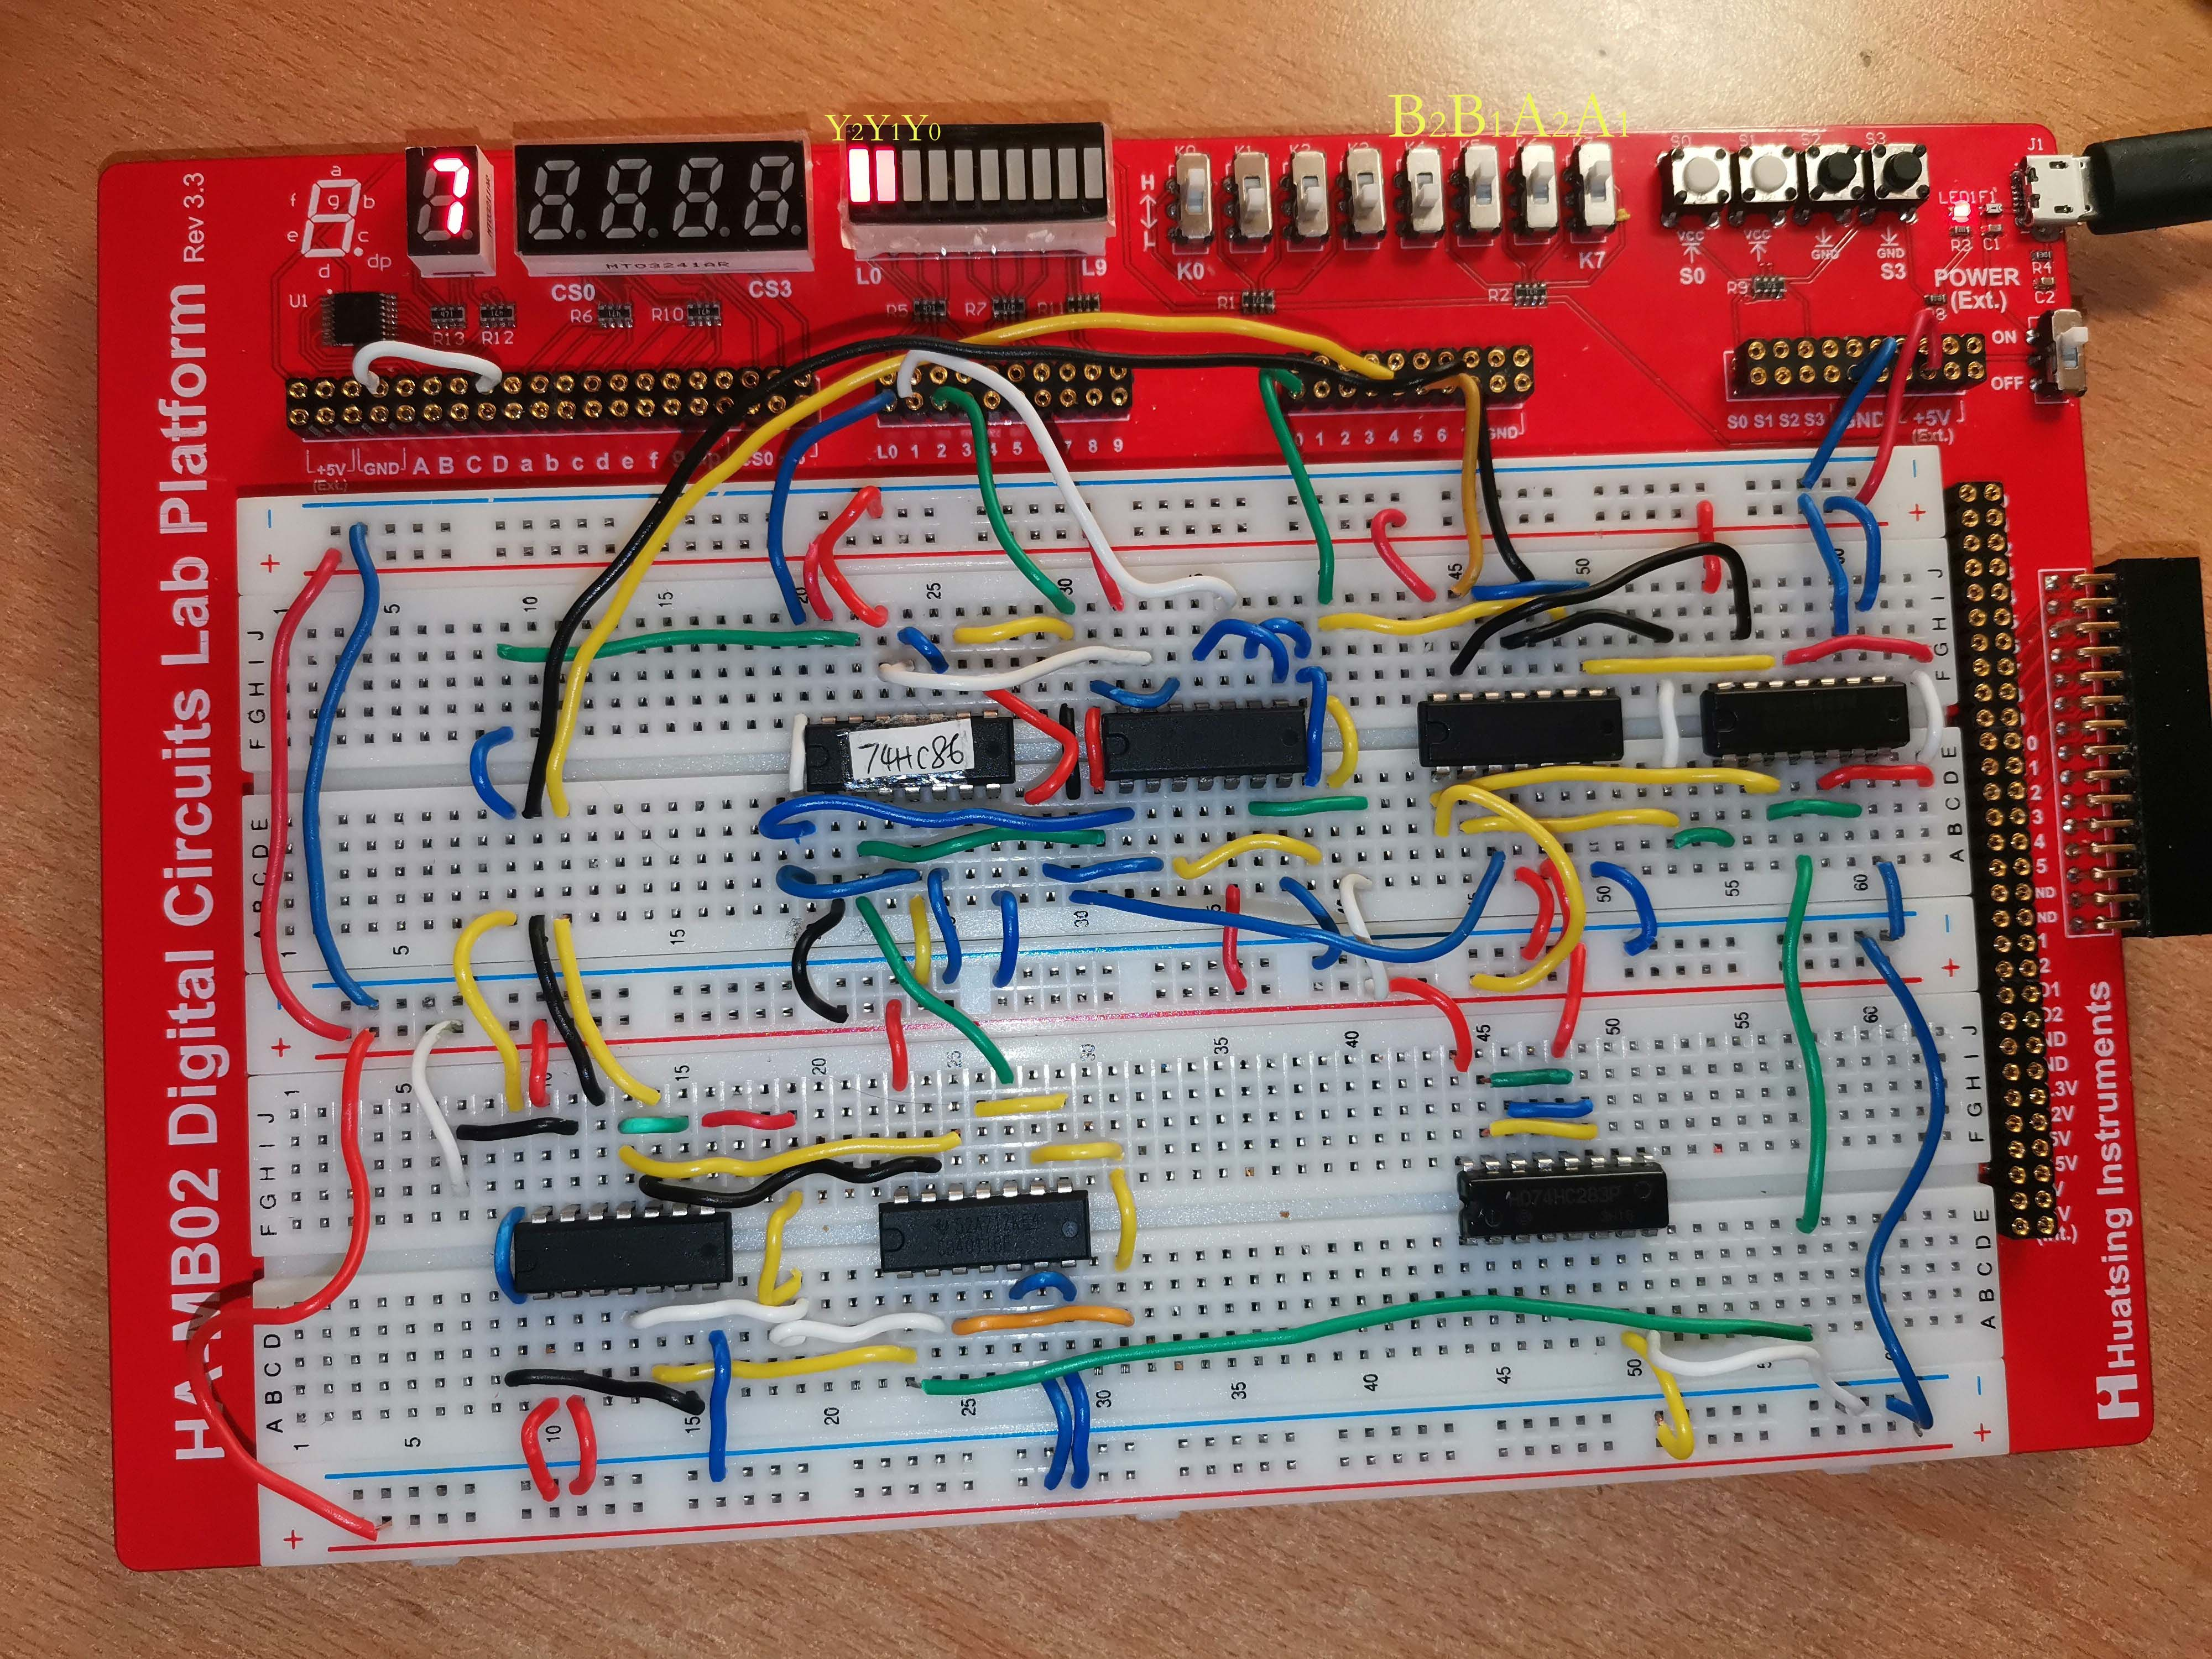
\includegraphics[scale=0.04]{1-3'.jpg}}\hspace{0.3mm}
    \subfigure[2-3]{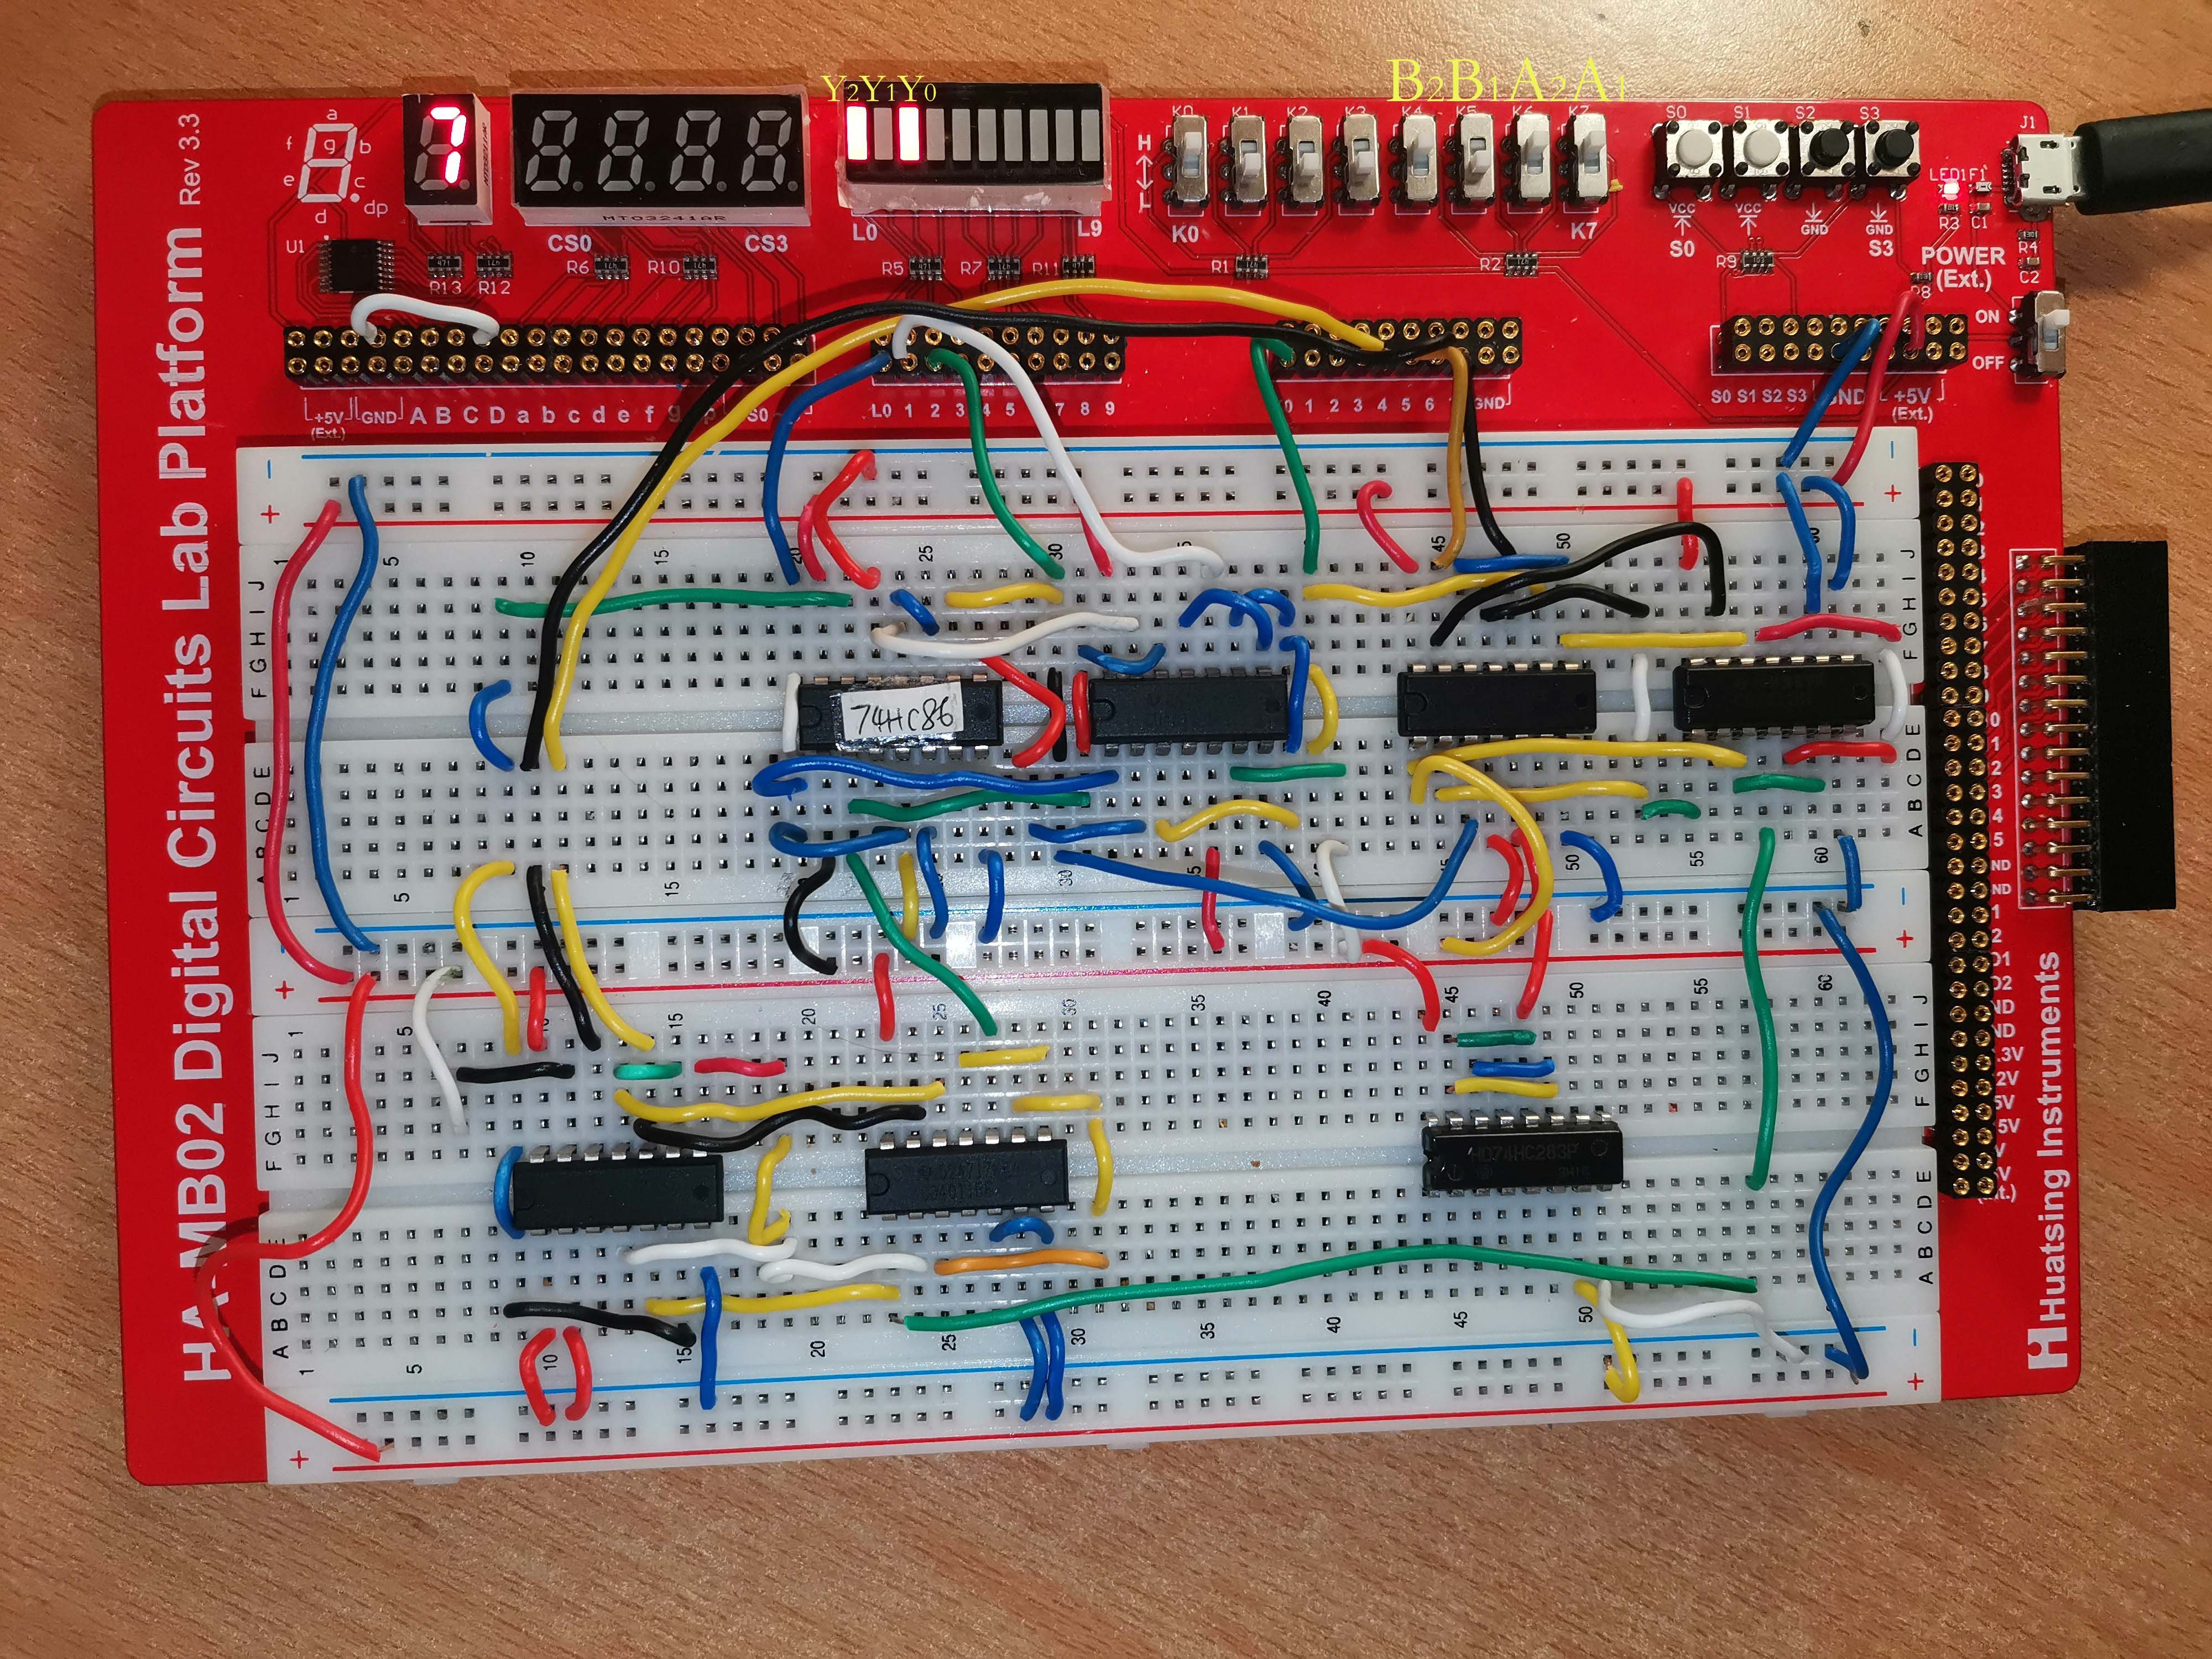
\includegraphics[scale=0.04]{2-3'.jpg}}\hspace{0.3mm}
    \subfigure[3-2]{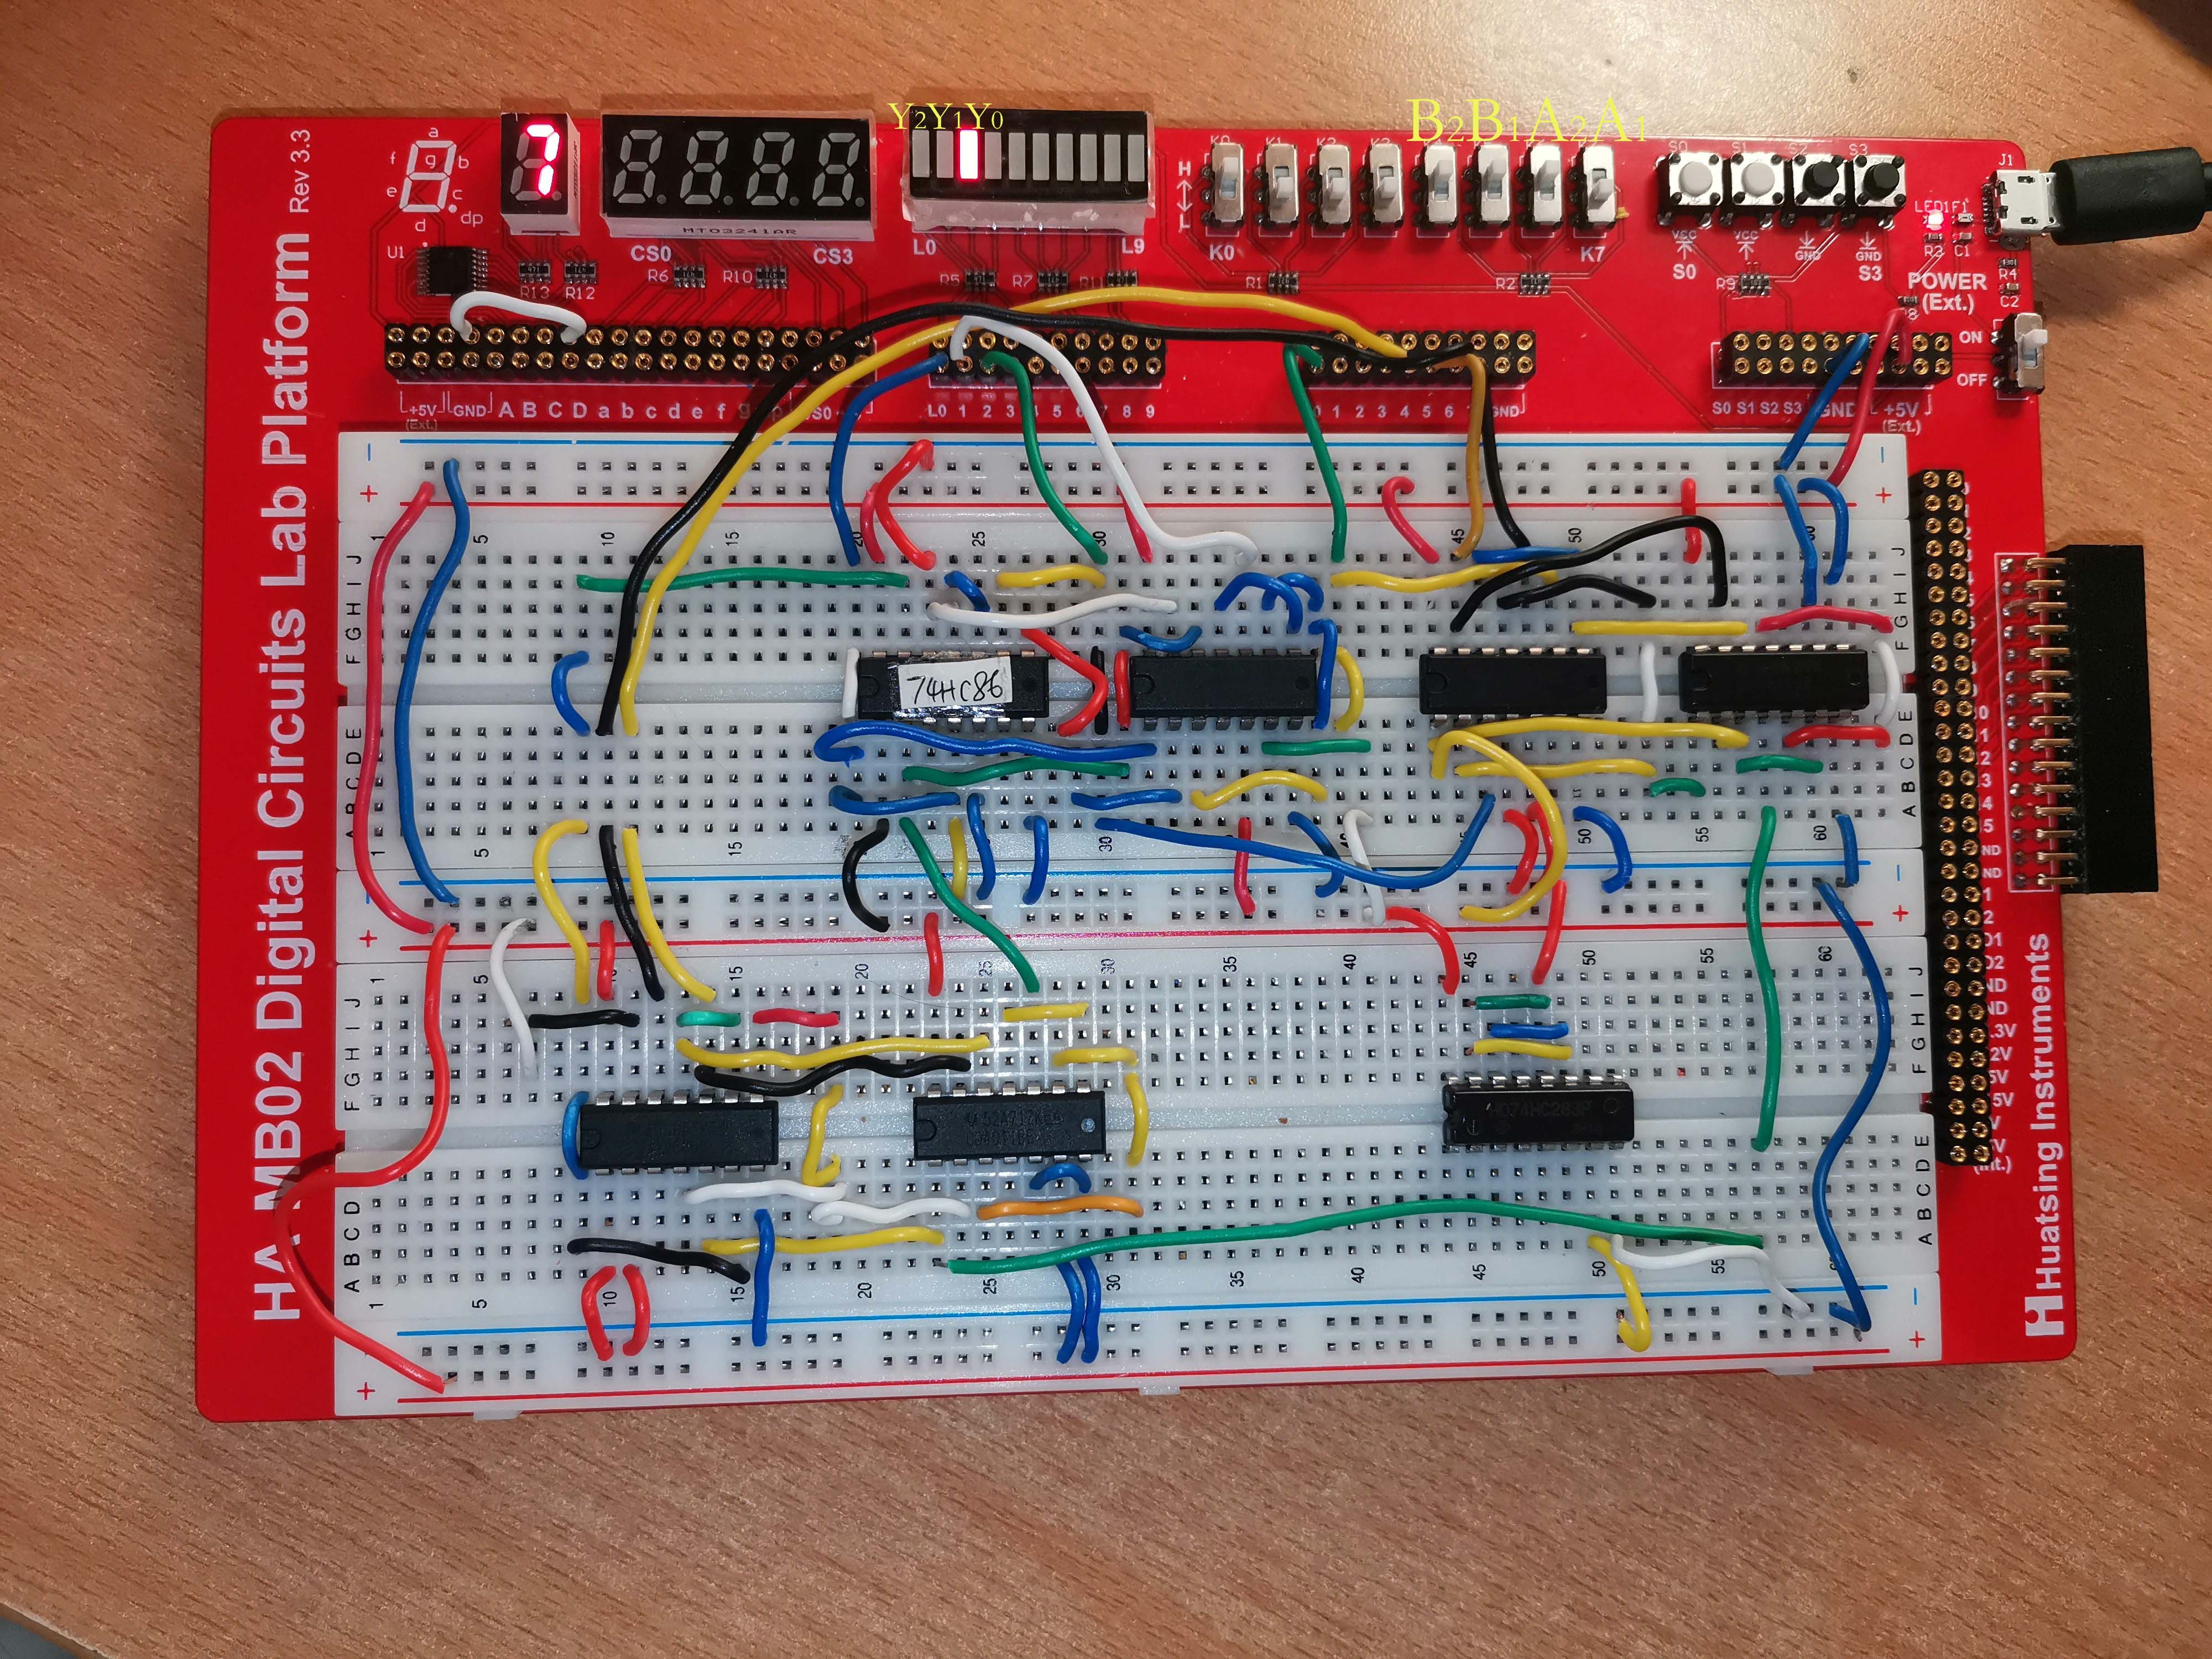
\includegraphics[scale=0.04]{3-2'.jpg}}\hspace{0.3mm}
    \caption{显示原码的二位减法器}
    \restoregeometry
    }
\end{figure}\par

\section{用加法器芯片实现加法运算}
\subsection{电路设计}
考虑到74HC283是四位加法器,我们只需要完成两位加法,因此将A4、A3、B4、B3置零,同时将进位输入CI置零,并将A2、A1、B2、B1端分别与输入相连,那么输出$S_3S_2S_1$即为A和B求和后的二进制数(求和结果不大于6,即最多为三位二进制数). 将$S_3S_2S_1$分别和数码管的二进制输入端口$CBA$相连接,而求和结果不大于6,于是最高位$D$置零,如此就设计好了电路.\par
具体的电路图如下:
\begin{figure}[H]\centering
    {
        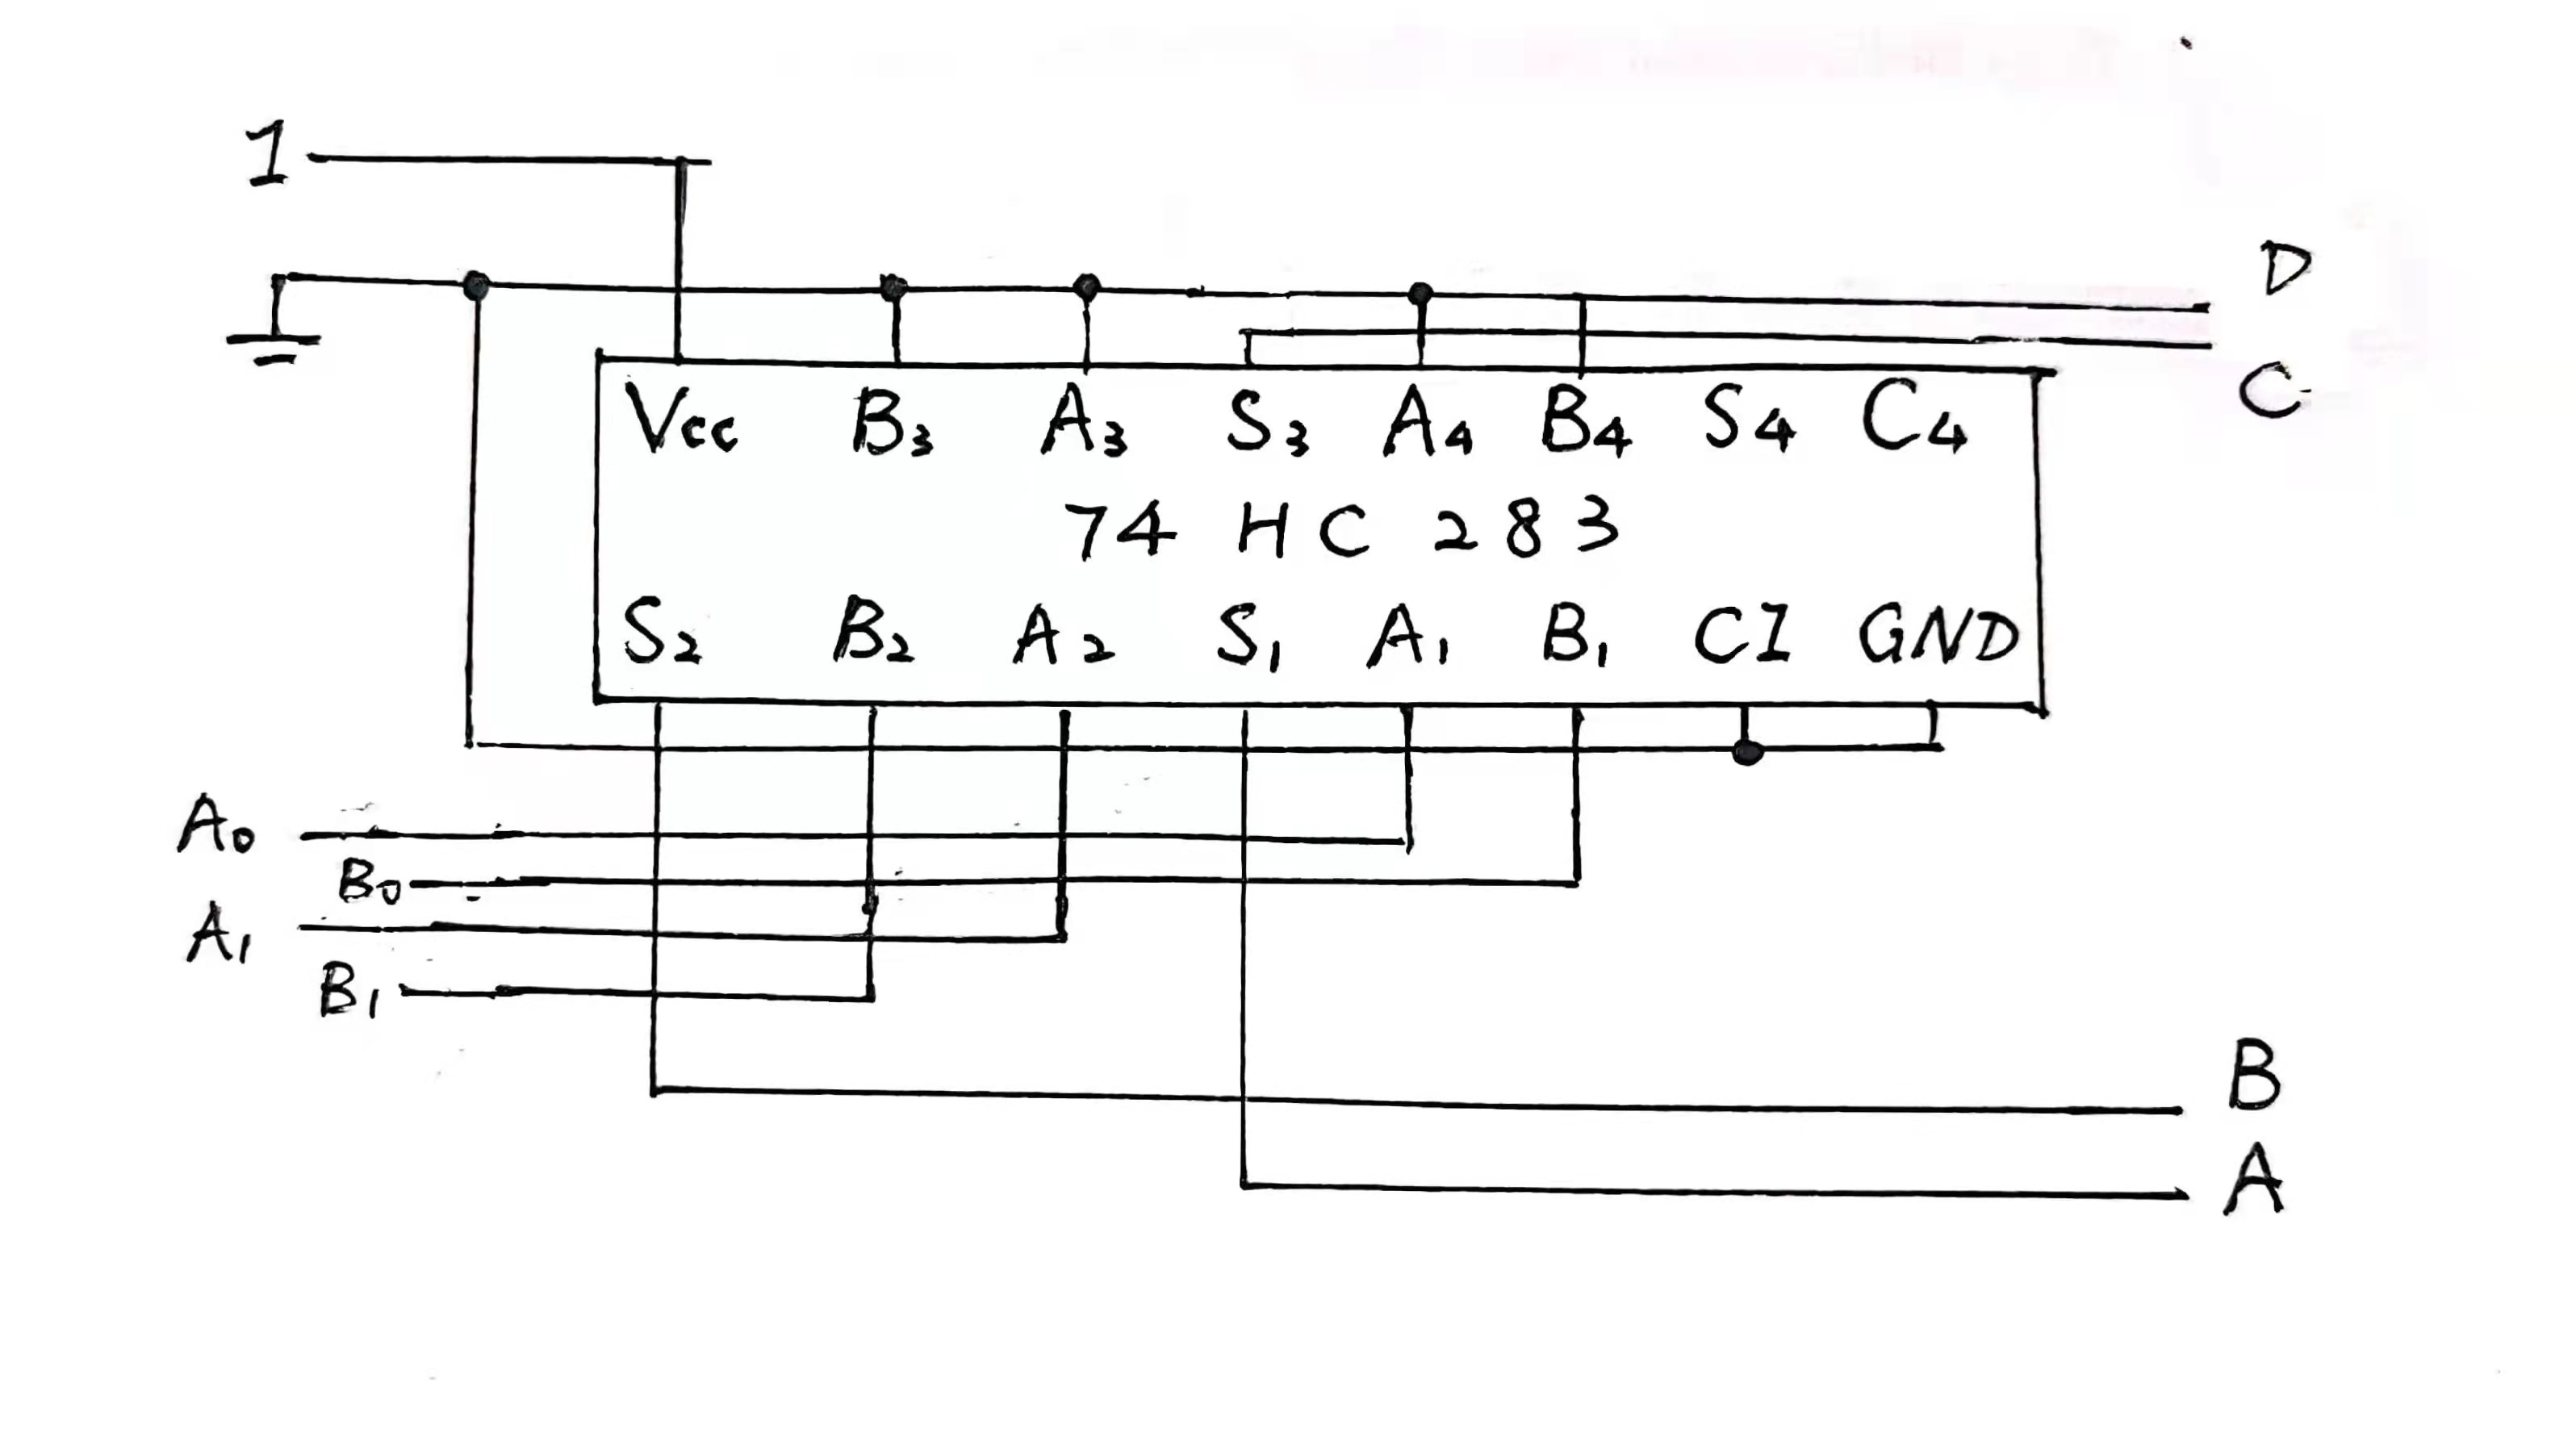
\includegraphics[scale=0.1]{7.jpg}
        \caption{加法器芯片实现加法运算器电路图}
    }
\end{figure}\par
\subsection{电路实物图}
\begin{figure}[H]\centering
    {
        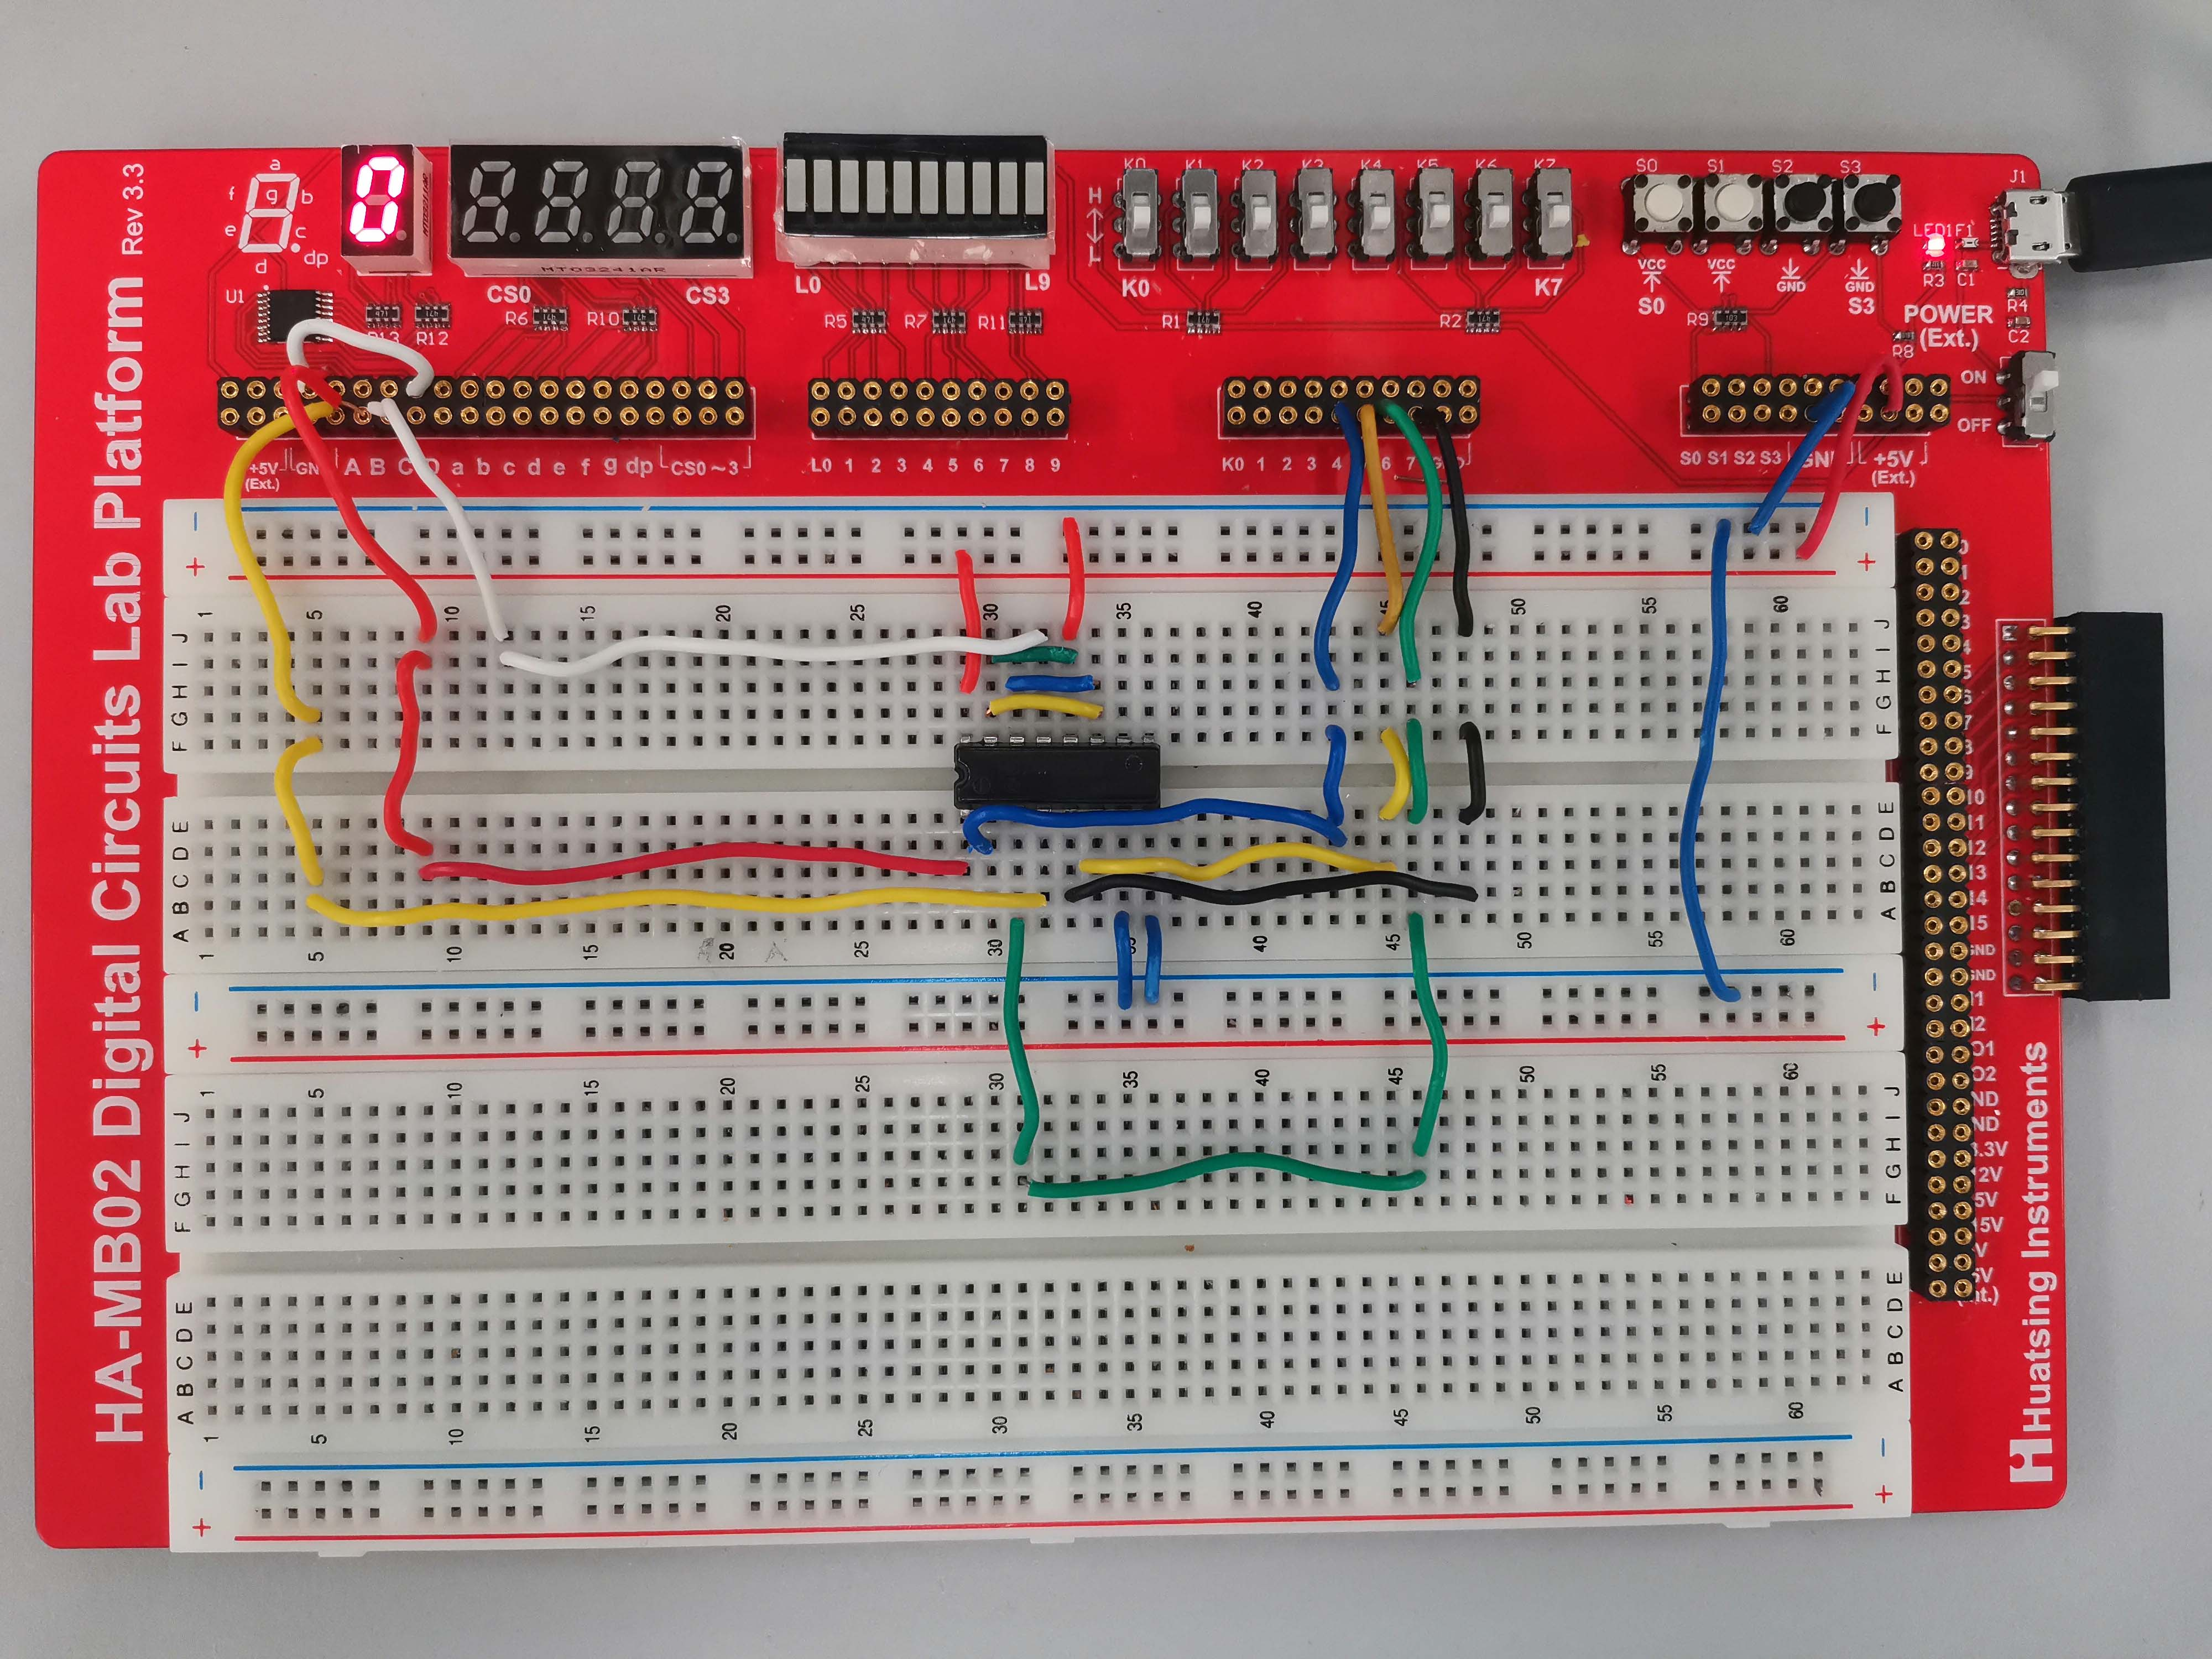
\includegraphics[scale=0.06]{30.jpg}
        \caption{用74HC283实现的加法器}
    }
\end{figure}\par
\vspace{-2em}
\subsection{功能展示}


\begin{figure}[H]\centering
    {
    \setcounter{subfigure}{0}
    \newgeometry{a4paper,left=3cm,right=0cm}
    \vspace{-1em}
    \subfigcapskip=-10pt
    \subfigure[0+1]{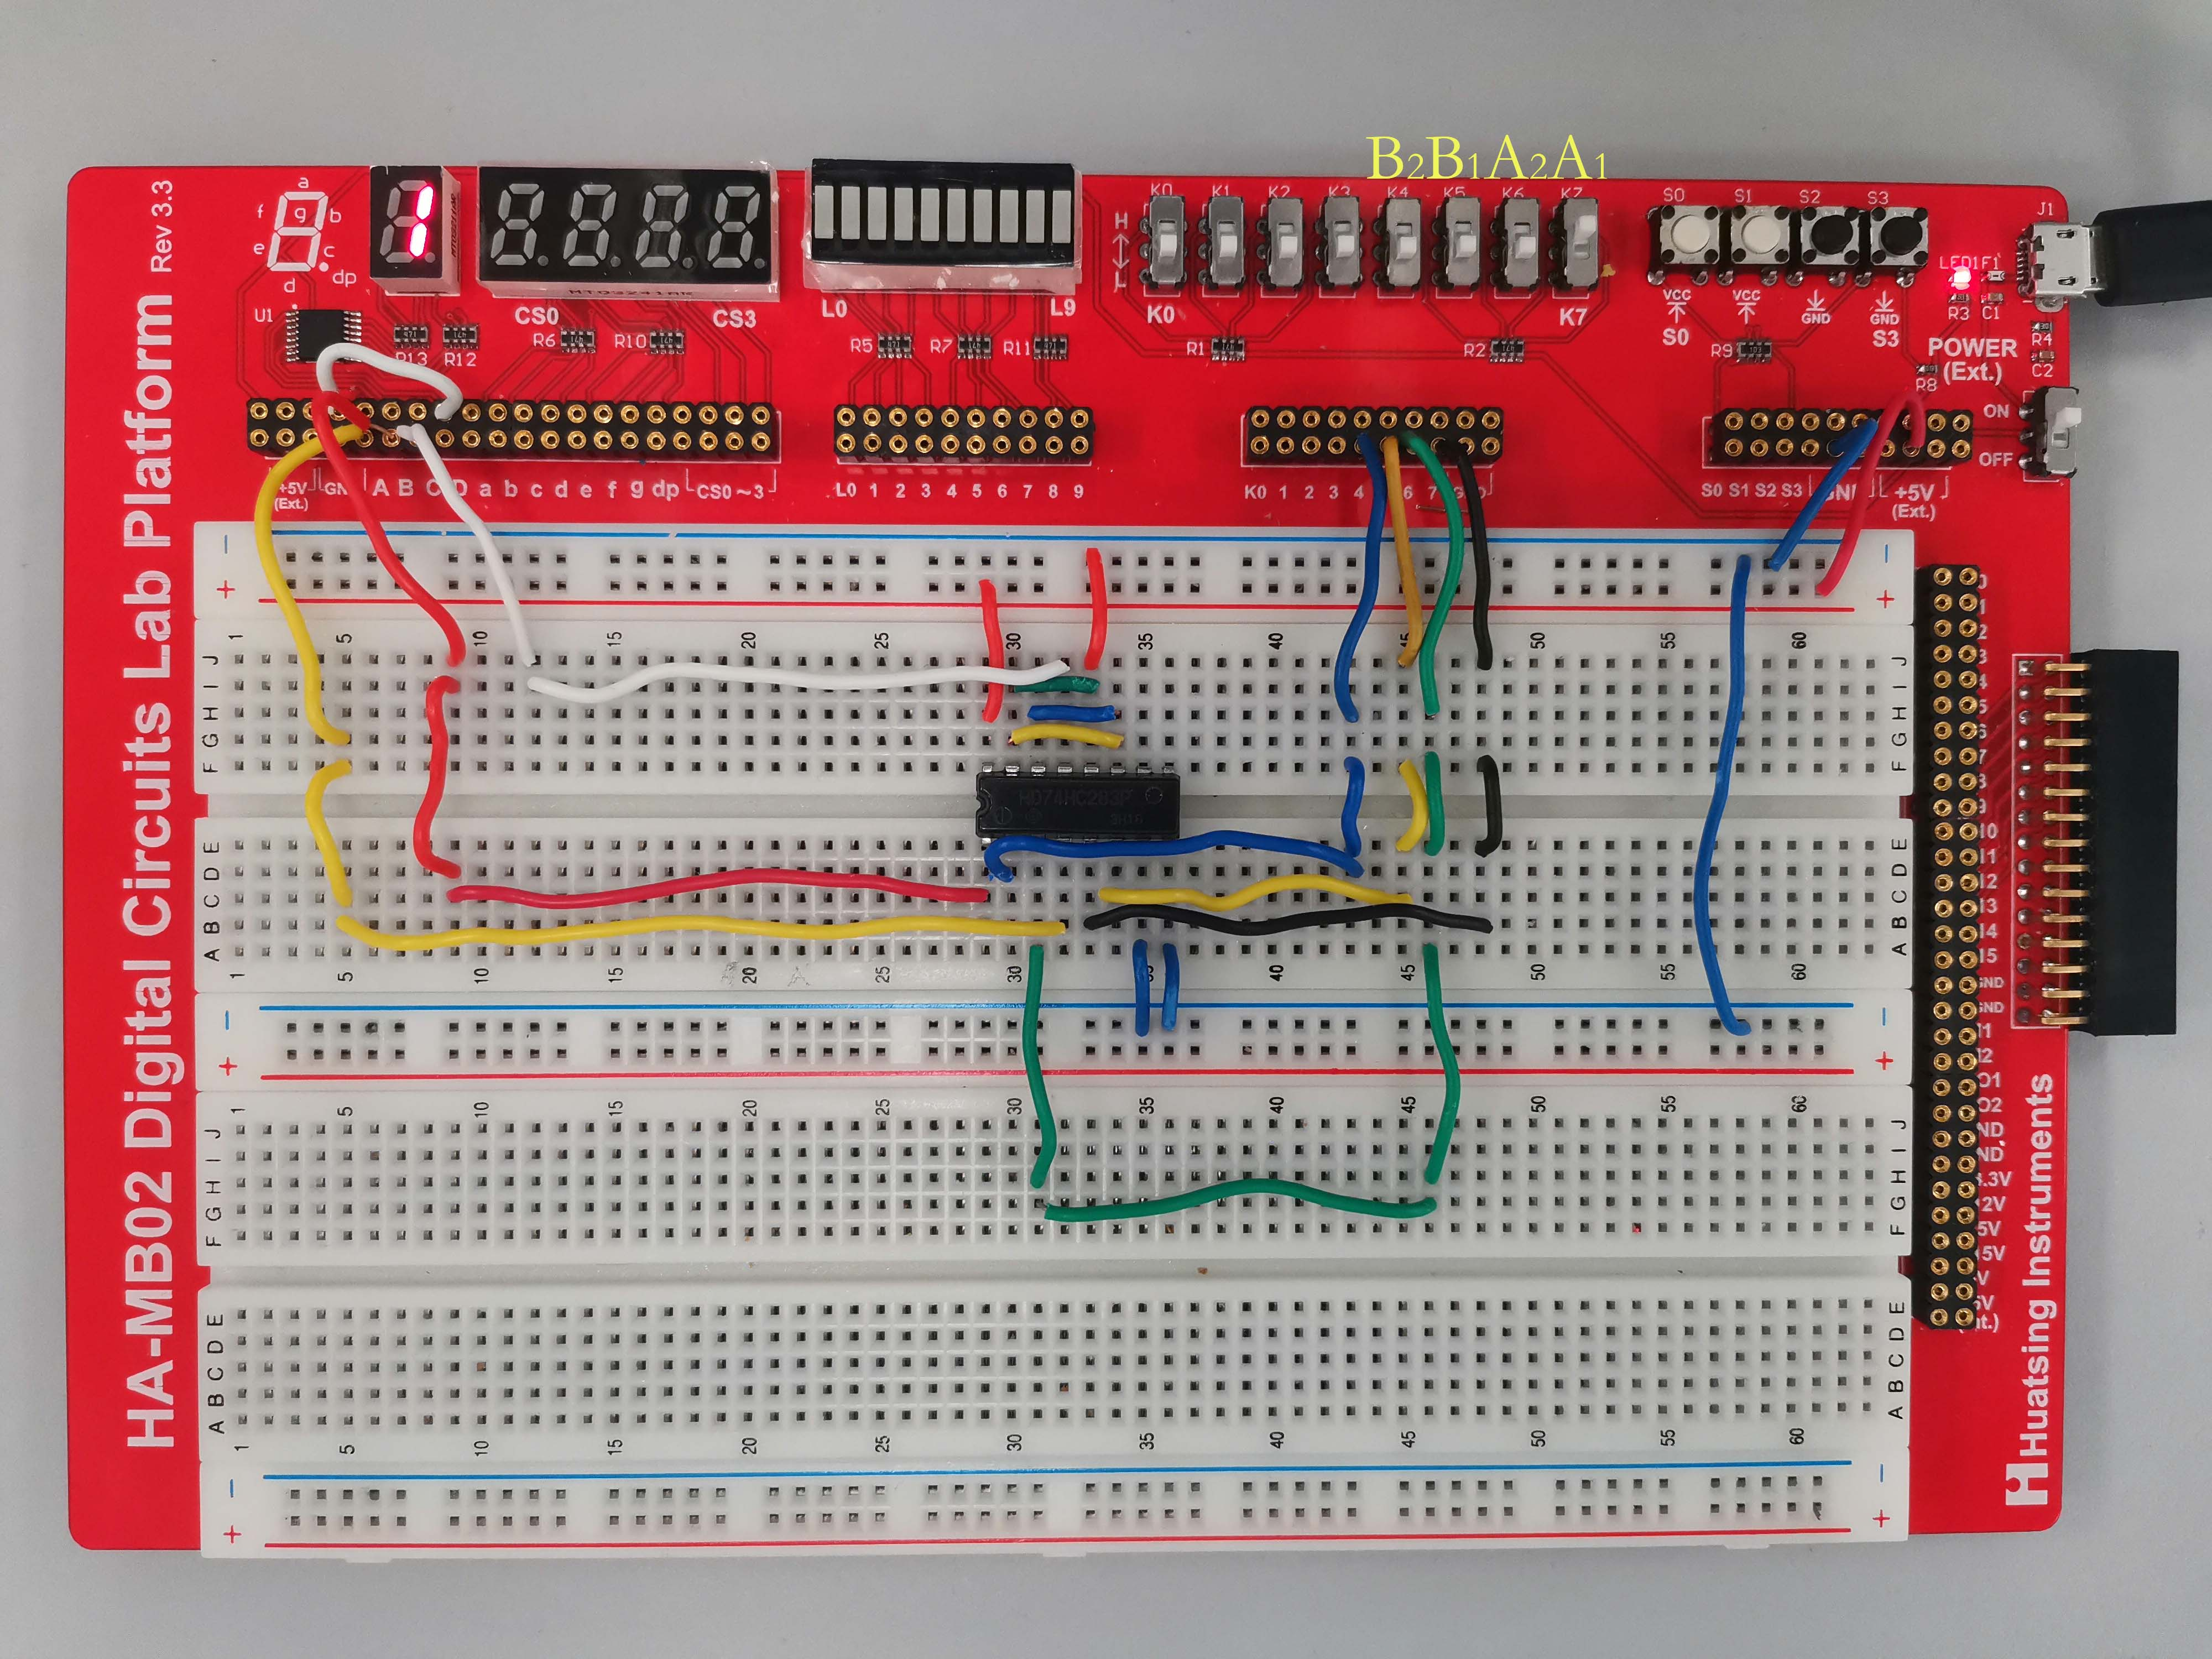
\includegraphics[scale=0.04]{0+1'.jpg}}\hspace{0.3mm}
    \subfigure[1+1]{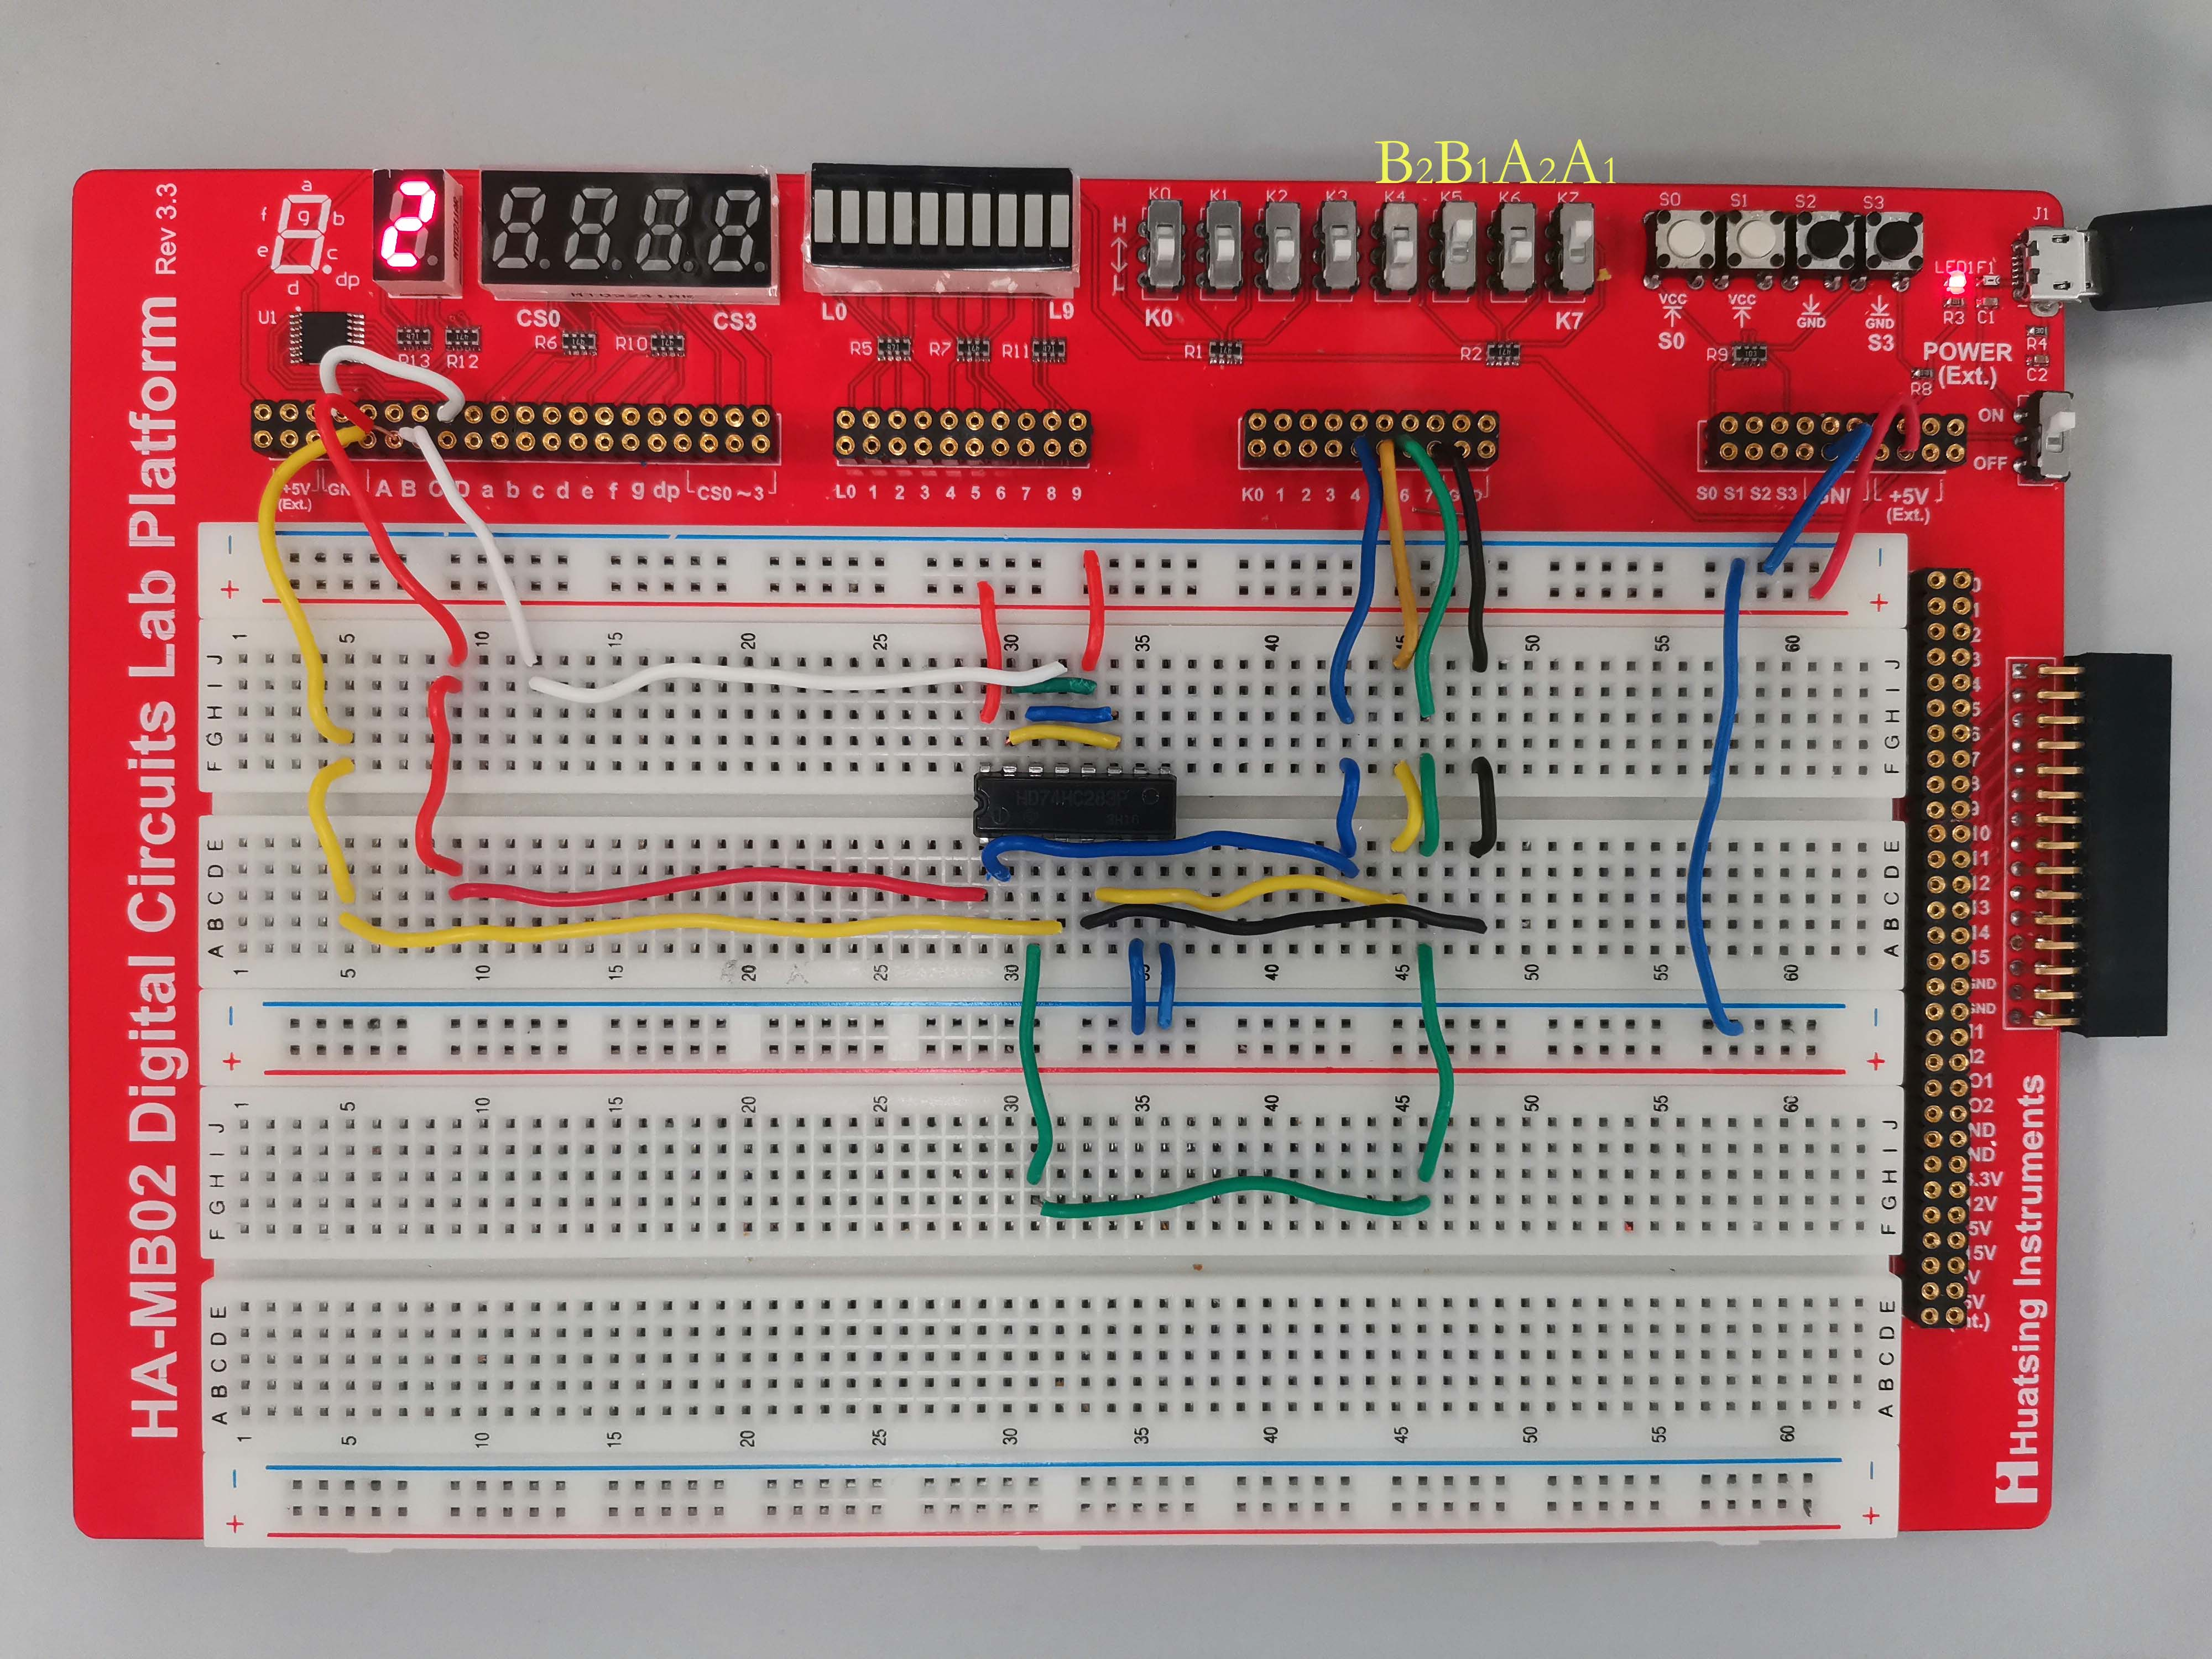
\includegraphics[scale=0.04]{1+1'.jpg}}\hspace{0.3mm}    
    \subfigure[1+2]{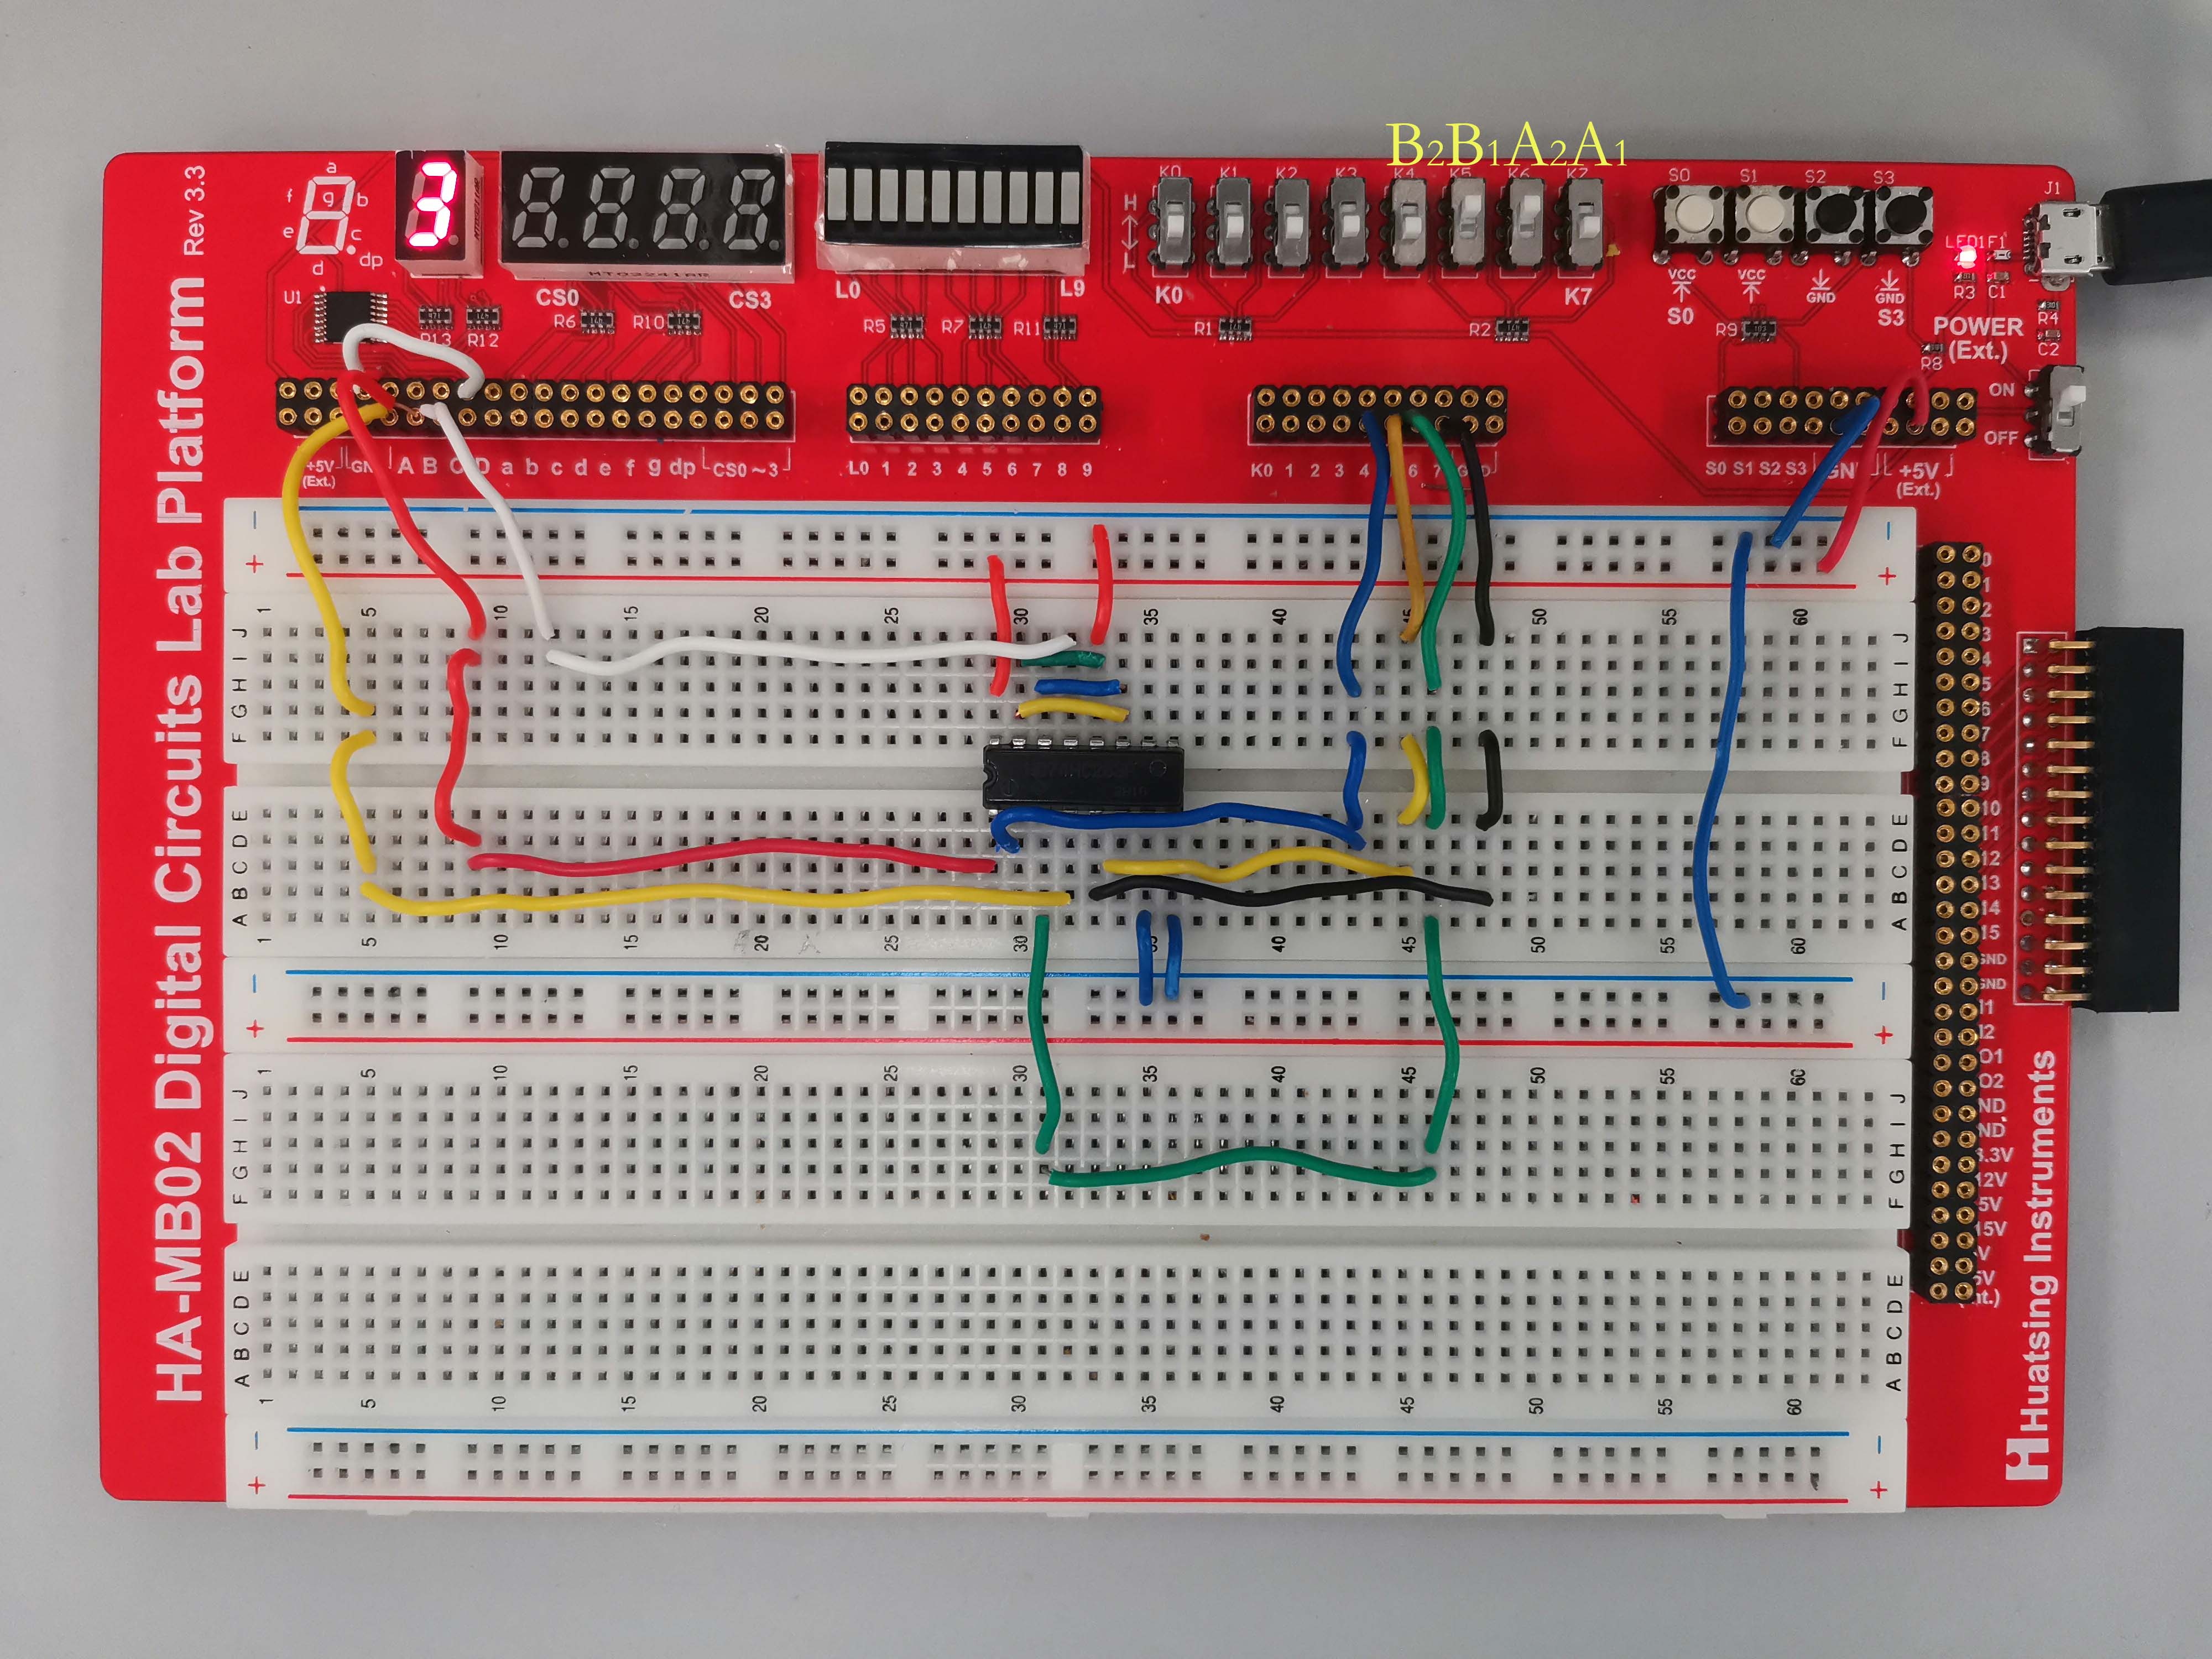
\includegraphics[scale=0.04]{1+2'.jpg}}\hspace{0.3mm}
    \subfigure[1+3]{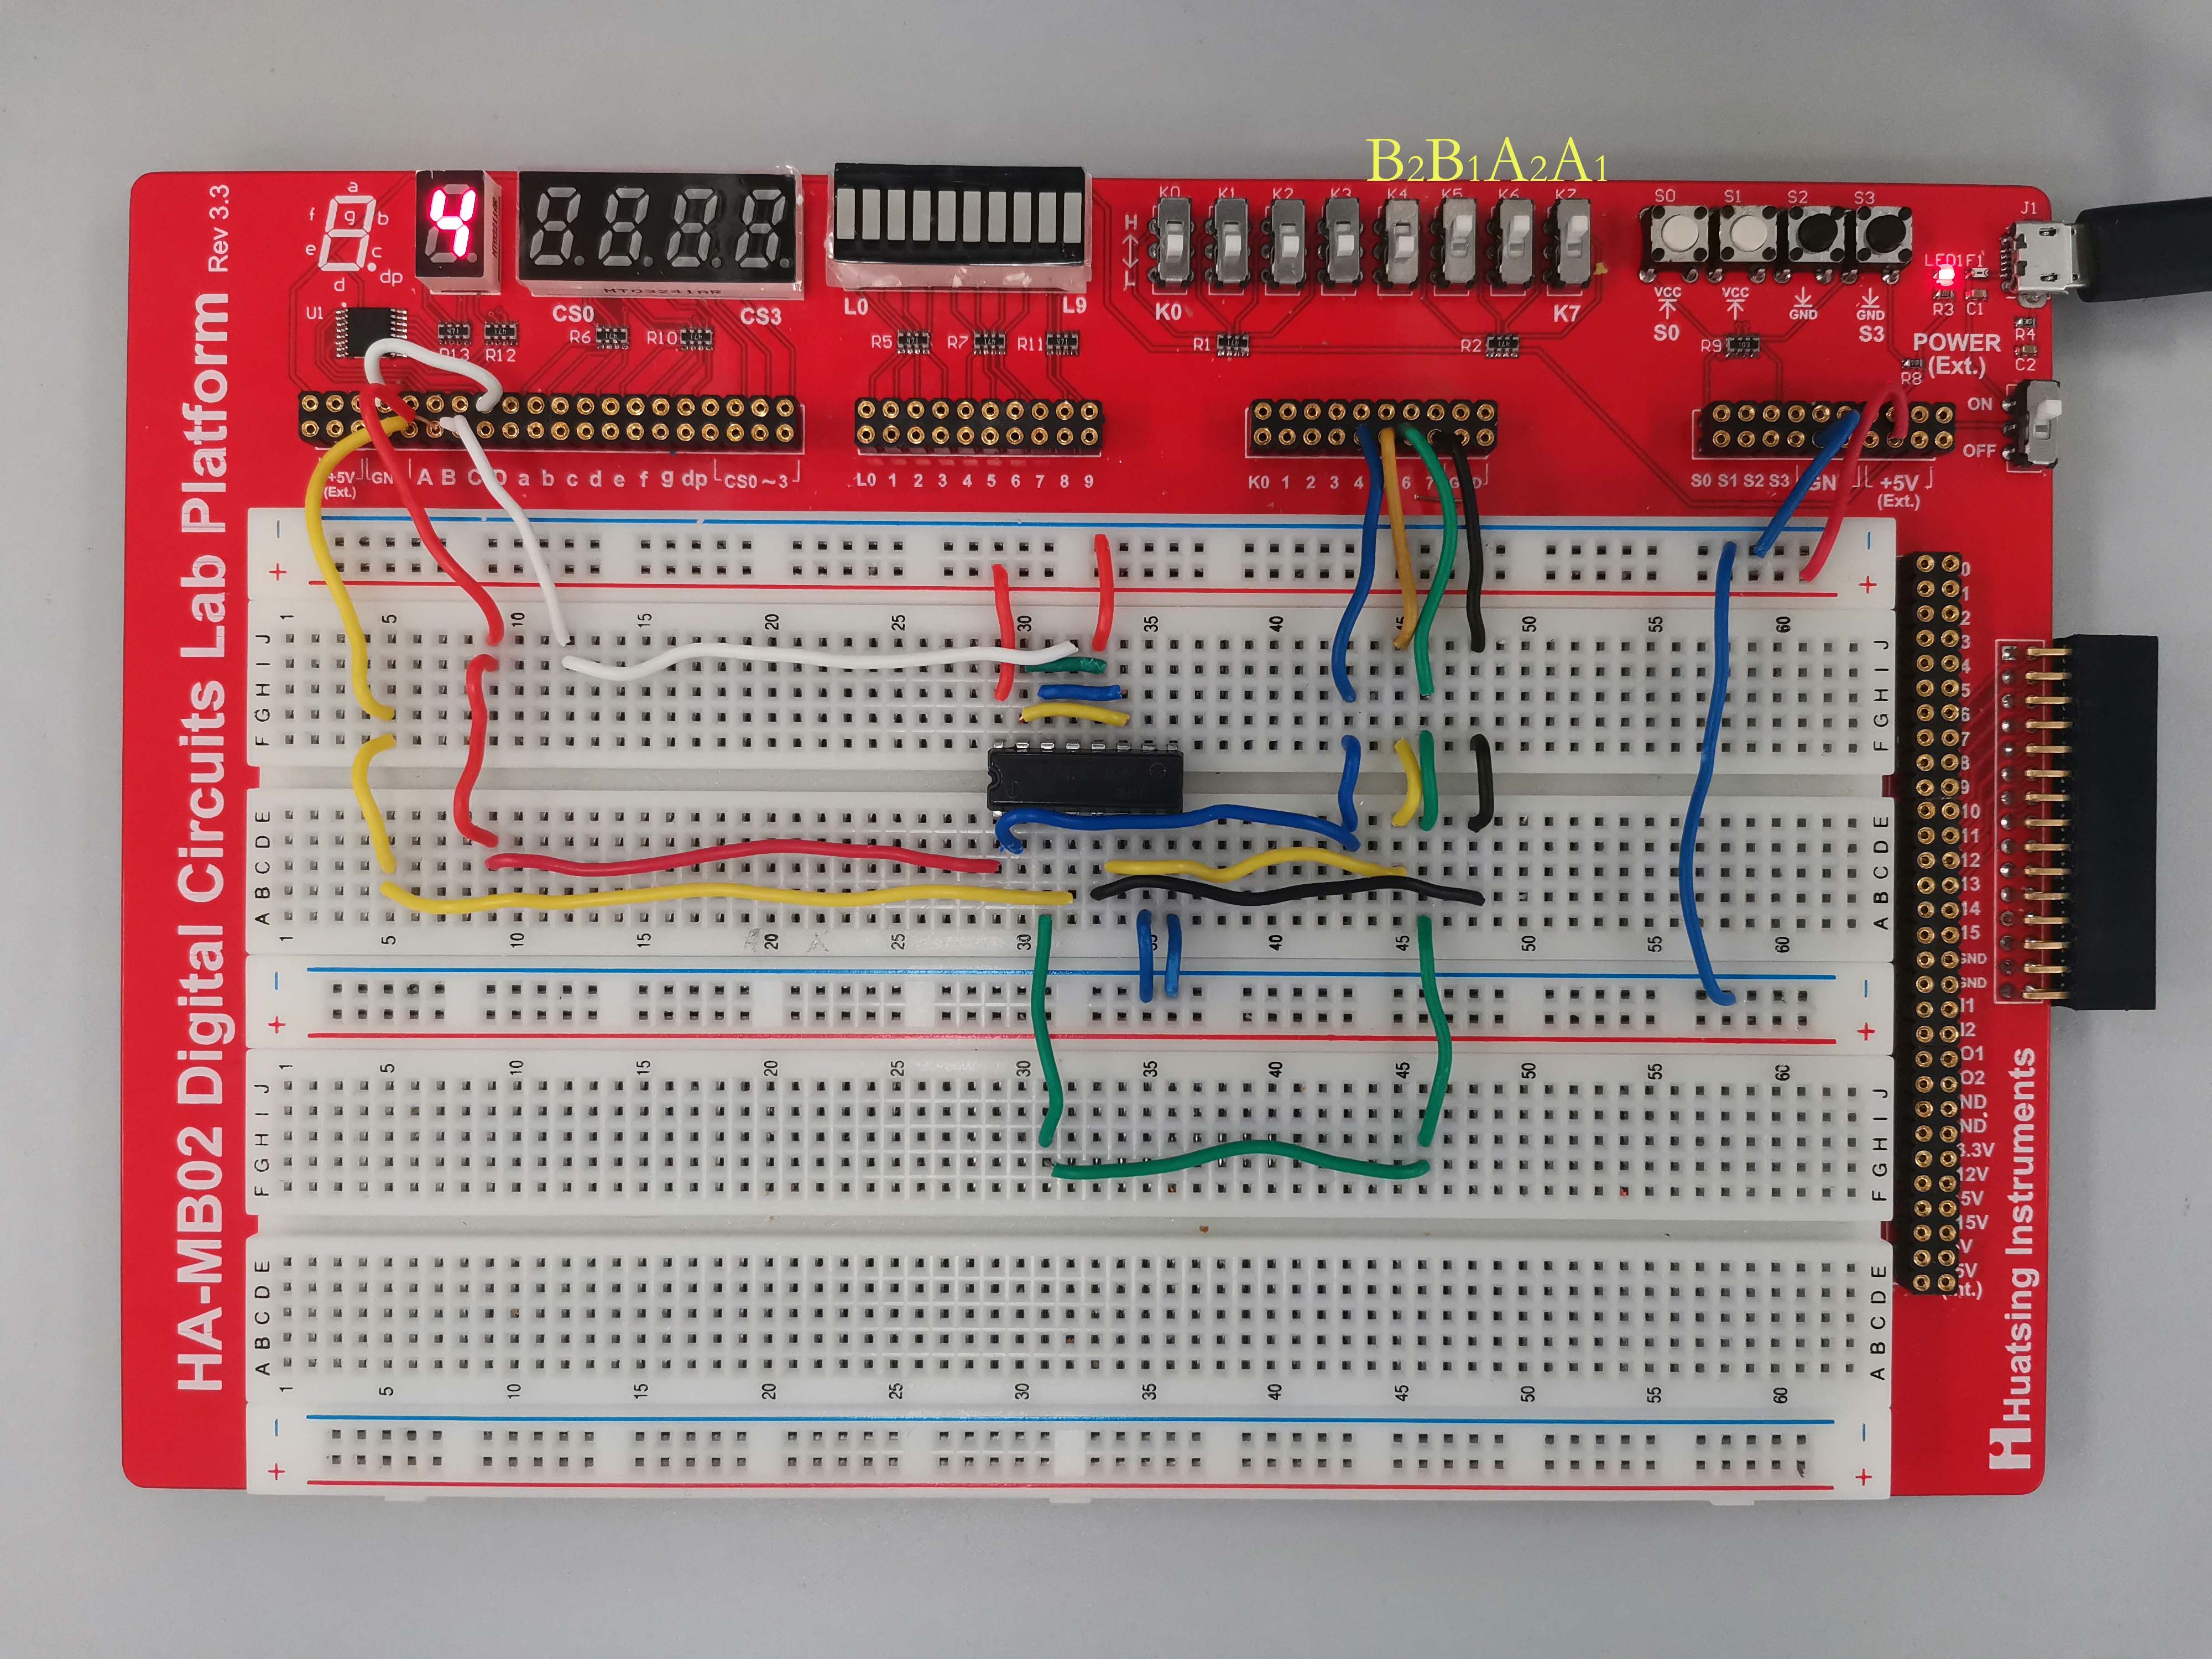
\includegraphics[scale=0.04]{1+3'.jpg}}\hspace{0.3mm}
    \subfigure[2+3]{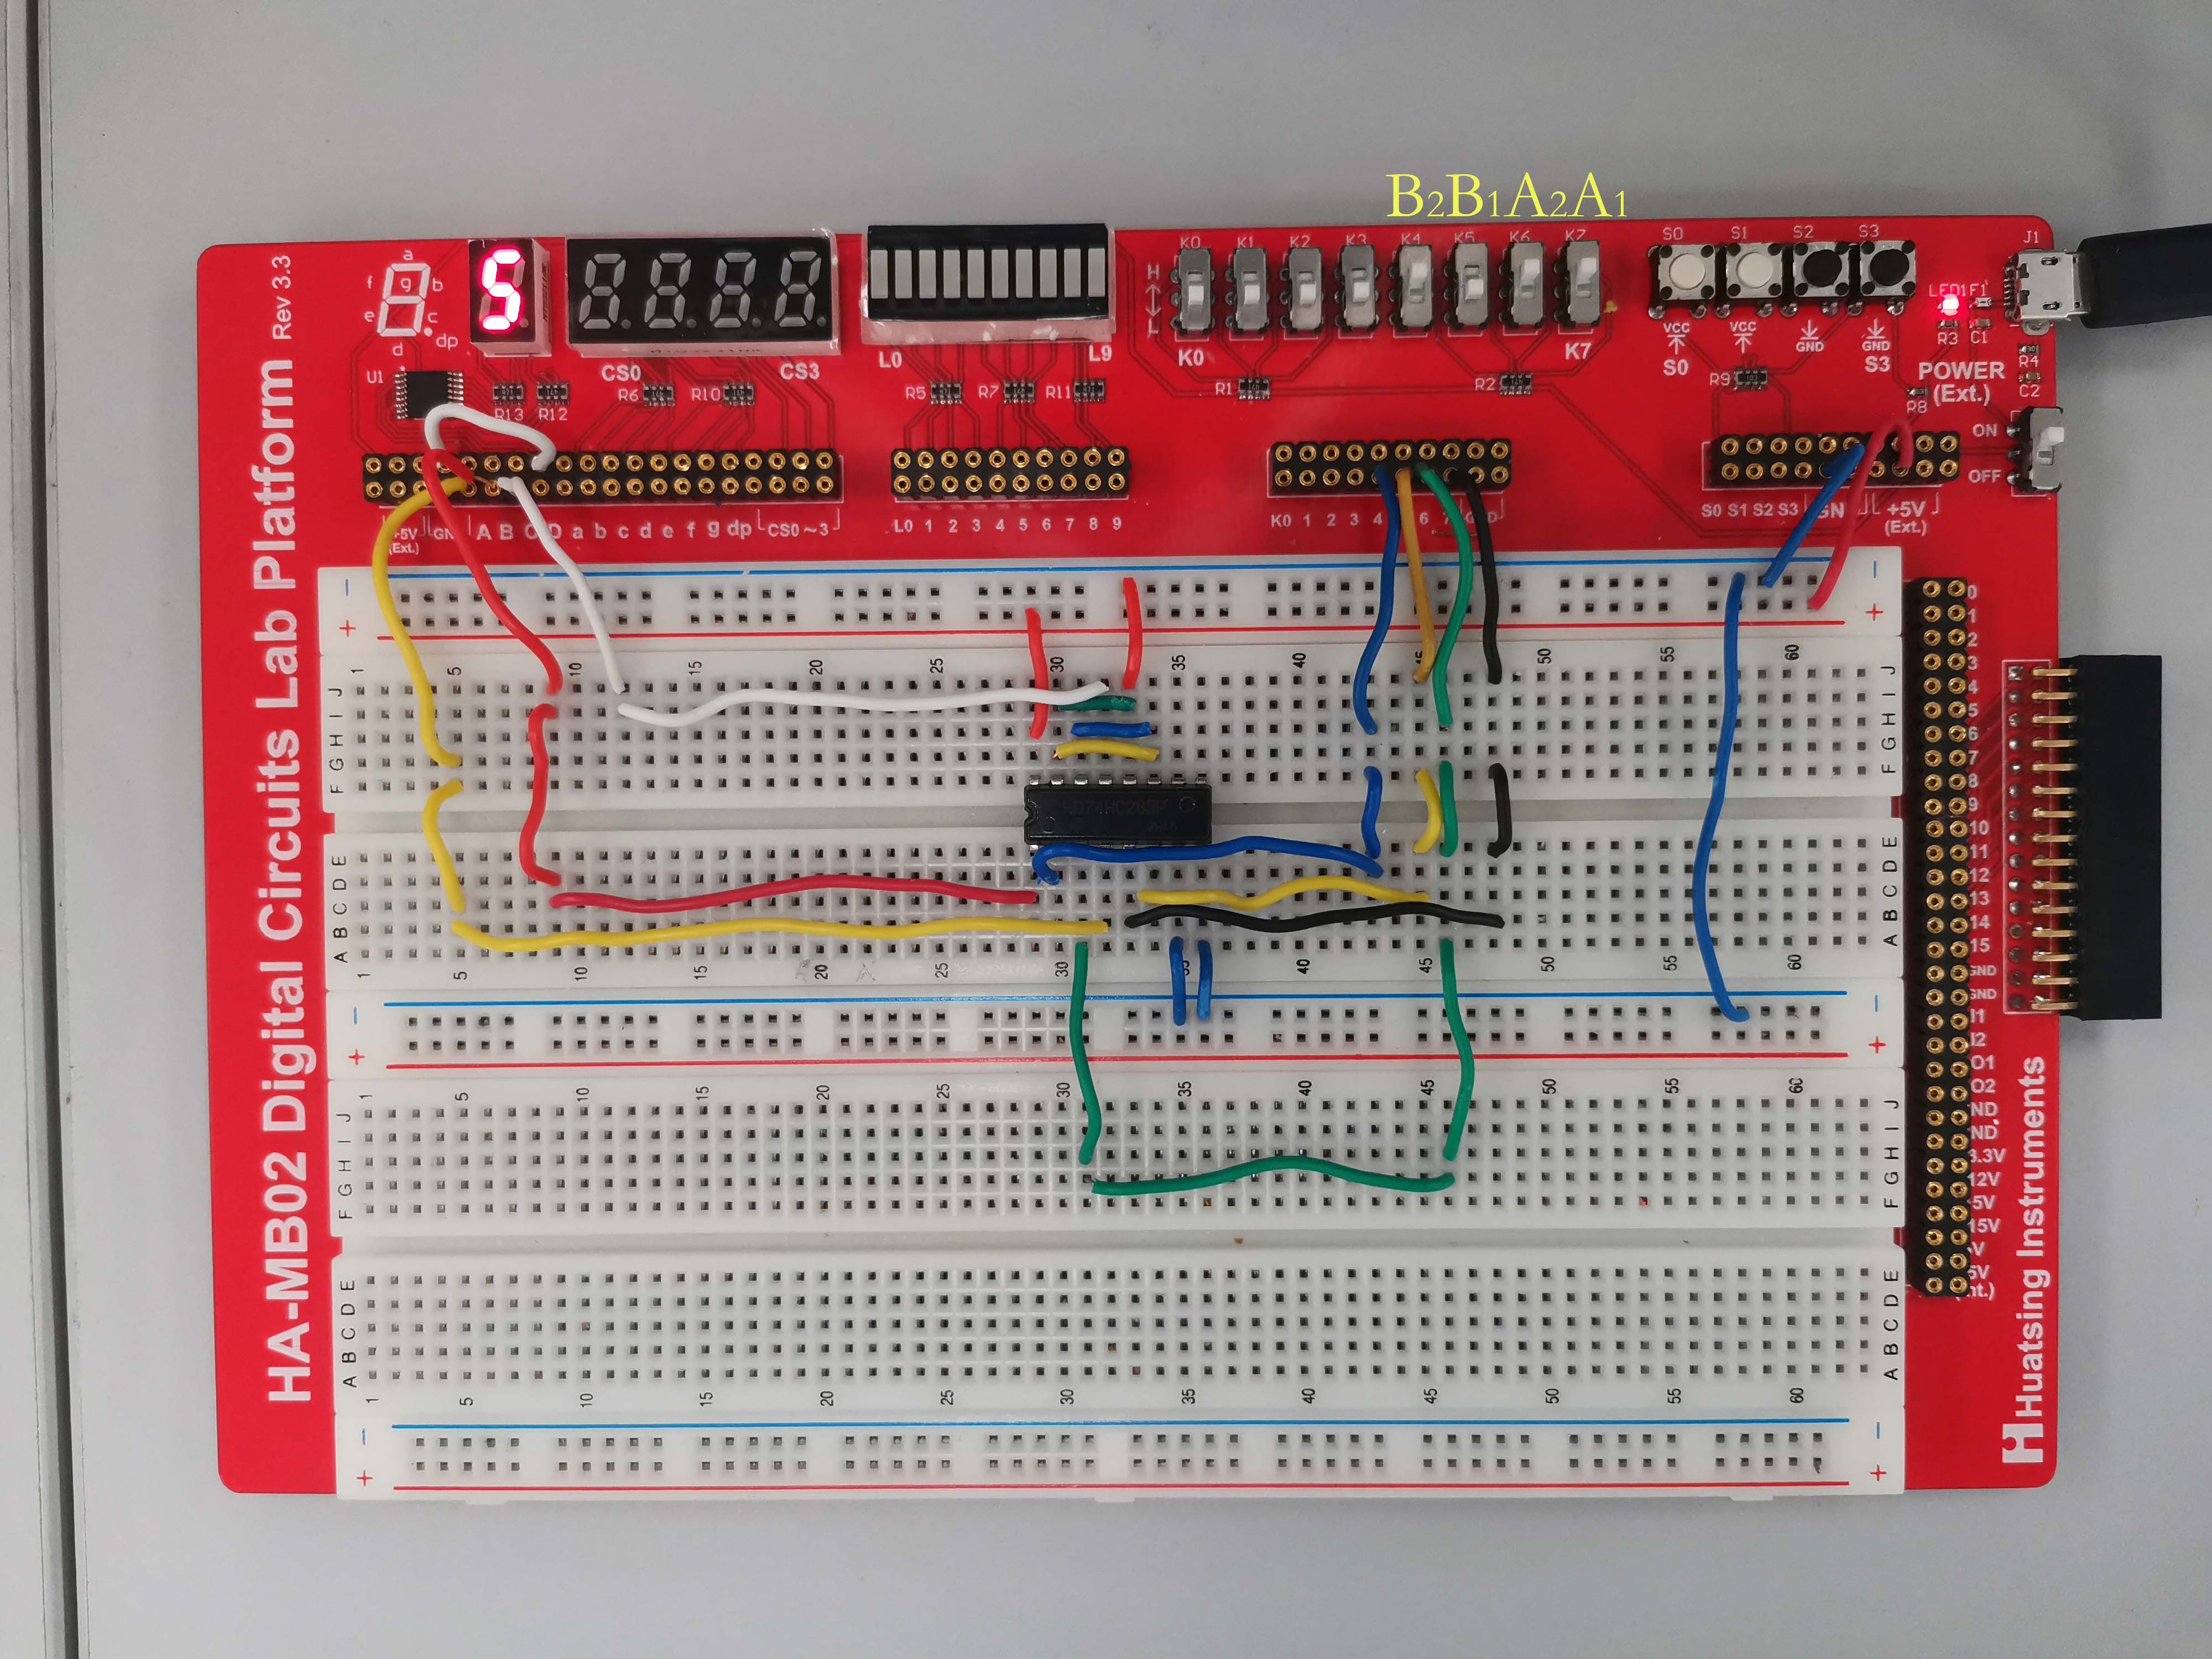
\includegraphics[scale=0.04]{2+3'.jpg}}\hspace{0.3mm}
    \subfigure[3+3]{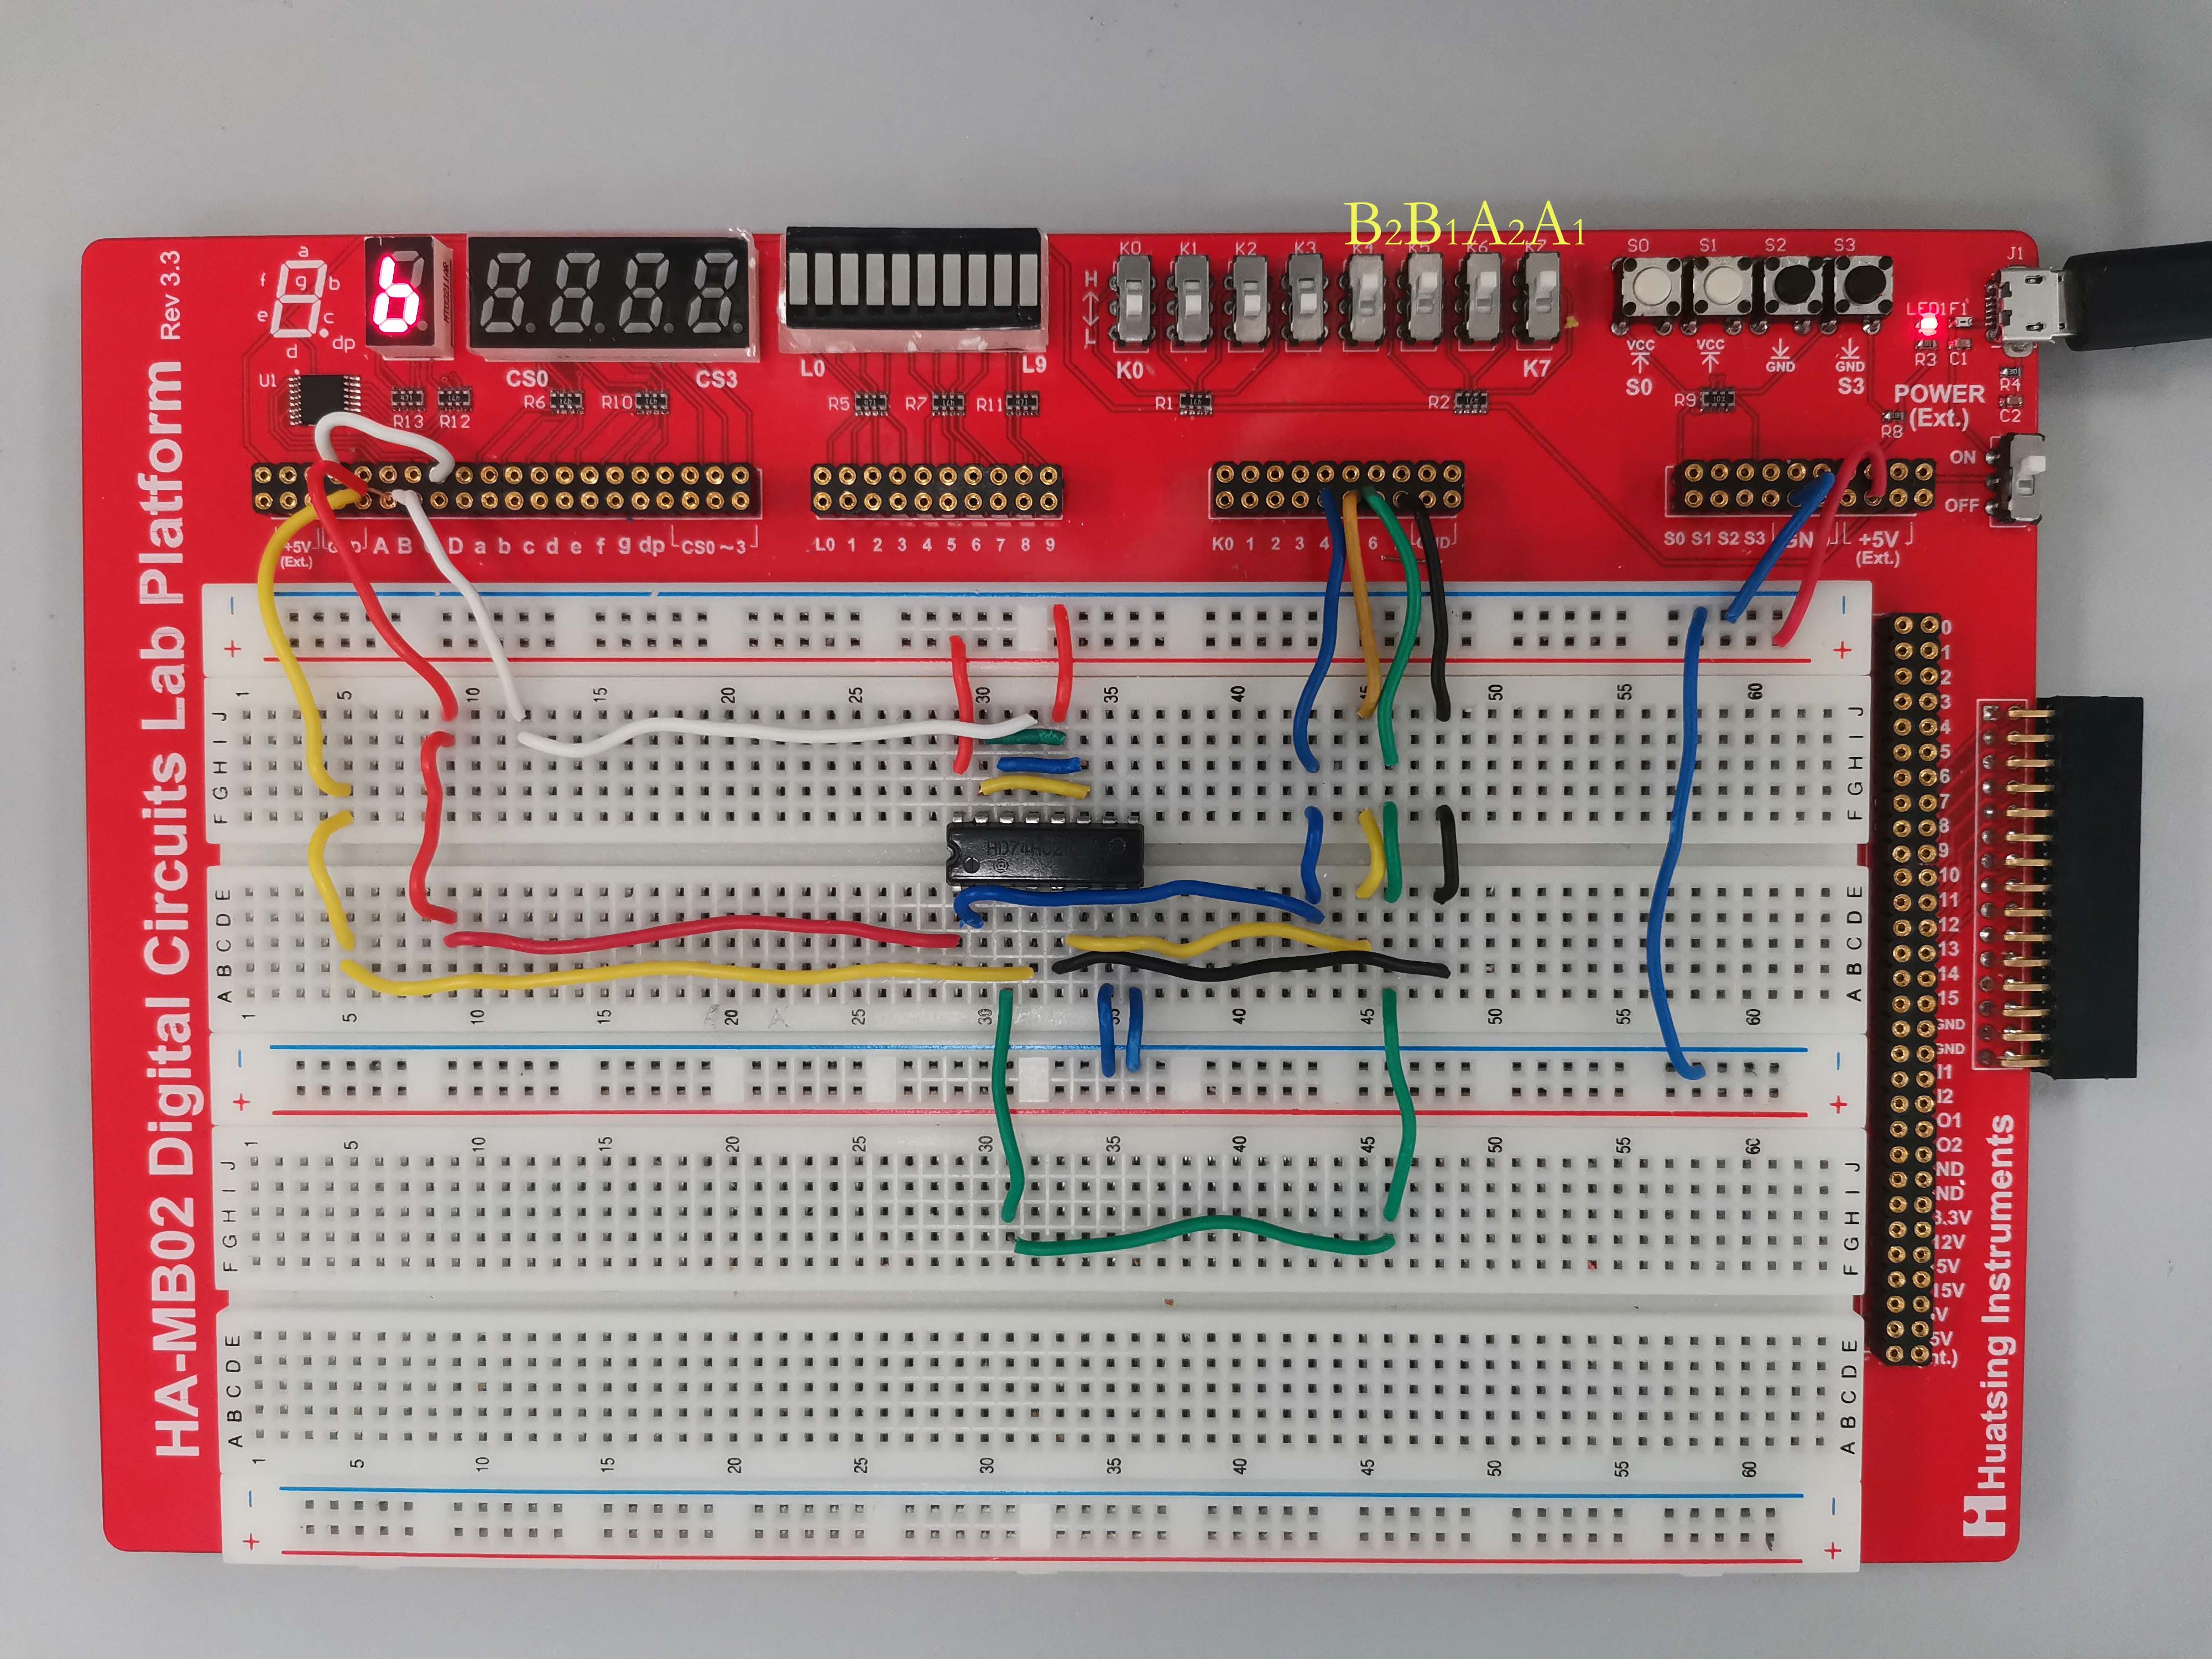
\includegraphics[scale=0.04]{3+3'.jpg}}\hspace{0.3mm}
    \caption{用74HC283实现的加法器功能展示}
    \restoregeometry
    }
\end{figure}\par

\section{问题及其解决方法}

\subsection{将电路图移植到面包板上时节点、接线混乱}
一开始接线时,面对电路图,我时常将各个节点、线路搞混,不得不拆掉重接. 然而我后来发现,面包板上每个节点都有对应坐标,可以在线路图上用纸标记各个节点、线路的坐标,从而更有利于实现任务.

\subsection{面包板上排线布局不合理}
一开始我规划最基础的加法器时,将芯片全部集中在了右上角,并将右上角通路堵得异常严实,导致出线和入线都格外困难,无法再向其中加入新功能;后来,我修改了部分芯片和排线的布局,将其合理规划之后均匀分配到整块面包板上,最终才得以完成任务. 可见,在接手问题时应该对问题全貌有宏观的把握,这样才能保证任务的顺利完成.

\subsection{发光二极管显示不稳定}
我发现连接好电路后,发光二极管的示数十分不稳定,经常出现显示出错、显示结果跳动的情况. 初期我以为是连线不稳的问题,后来查询芯片数据手册、与同学交流后才发现,芯片的输入端引脚不可悬空——这是电路由TTL构成的缘故. 在将输入端置0/1后,输出正确,这充分说明使用芯片时需要阅读说明书,查阅相关文献,不可想当然,必须充分认识元件的使用方法,才能更好地发挥元件的功能.

\subsection{对芯片的构造认识不足}
初始时,我忽略了芯片需要接入的$V_{DD}$和$GND$,并且把输入端、输出端搞混,因此产生了许多bug,最后一个个解决起来有不少困难. 因此,充分了解芯片特性是十分必要的.

\section{心得体会}
1. 实现运算器时,需要大量用到模块化设计电路的思想,进一步巩固了我在设计电路时对于元件的封装、调用等等技能的应用.\par
2. 掌握了搭接电路的基本技能,并且也培养了分析、检查电路的能力,更在完成任务的过程中培养了恒心和耐心.\par
3. 第一次用自己连接的元件和电线实现了简单的逻辑电路,使我更加意识到数电这门课程中实践、动手的重要性. 纸上得来终觉浅,唯有自己动一遍手,方才能更加深刻地领悟学习到的理论知识.

\end{document}
